\section{Analisi dei carichi del cinematismo}
Il meccanismo biella manovella è uno dei cinematismi più noti all’interno della meccanica applicata. \\
Il suo funzionamento è stato studiato negli anni attraverso diversi libri di testo. \\
\begin{figure}[h]
    \centering
    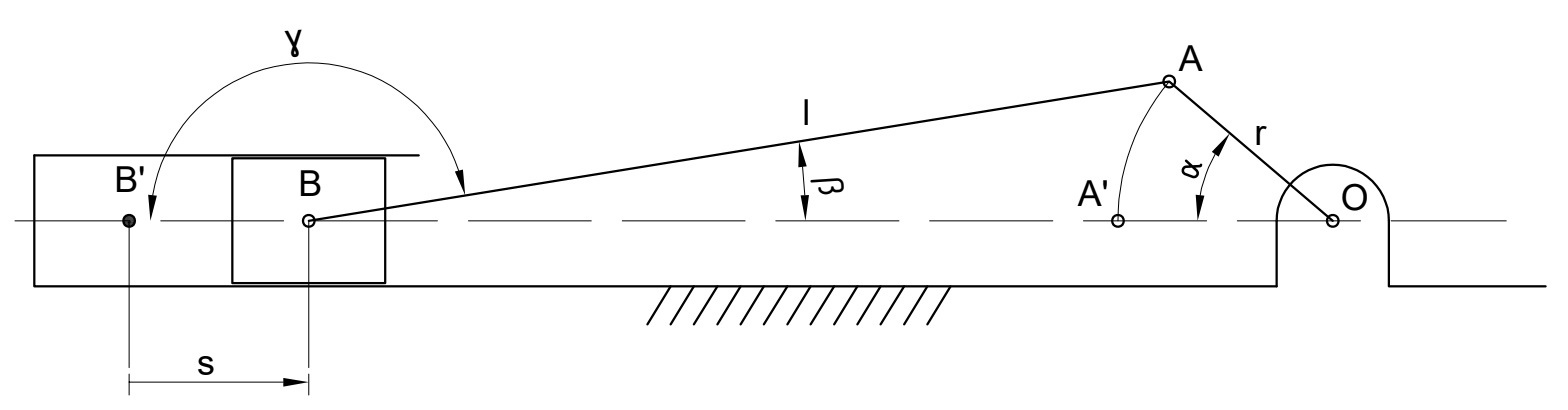
\includegraphics[scale=0.4]{Immagini/Cinematismo.png}
    \caption{Schema cinematismo biella-manovella}
    \label{fig:Cinematismo}
\end{figure}
\\
Si consideri il manovellismo in una posizione generica. \\
Nella figura mostrata si distinguono:
\begin{itemize}
   \item l lunghezza di biella 
   \item r raggio di manovella 
   \item $\alpha$ angolo di manovella 
	\item $\gamma$ angolo di inclinazione della biella 
	\item s spostamento generico del piede di biella 
\end{itemize}
\subsection{Andamento dello spostamento in funzione dell'angolo di manovella}
Si definisce la corsa s del pistone lo spostamento punto B da un punto morto B’, a cui corrisponde la posizione A’ del punto A.\\
Si indichi con $\alpha$ l’angolo che AO forma con il raggio AO’ e con l’angolo $\gamma$, l’angolo che AB forma con l’asse del moto di B. \\
Si indichi con r la lunghezza OA e con l la lunghezza AB.\\
Proiettando la spezzata BAO sull’asse del moto di B si ottiene:
\begin{equation}
    s=l+r+l\cos\left(\gamma\right)-r\cos\left(\alpha\right).
\end{equation}
Proiettando poi la stessa spezzata sulla direzione normale alla precedente eapplicando il teorema dei seni, si ottiene:
\begin{equation}
    l\sin\left(\gamma\right)=r\sin\left(\alpha\right)
\end{equation}
se si indica con $\lambda=\frac{l}{r}$ , diventa 
\begin{equation}
    \sin\left(\gamma\right)=\frac{1}{\lambda}\cdot\sin\left(\alpha\right)
\end{equation}
tenendo conto che $\gamma>\pi/2$
\begin{equation}
    \cos\left(\gamma\right)=-\sqrt{1-\frac{1}{\lambda^2}\cdot\left(\alpha\right)}.
\end{equation}
L’espressione di s diventa quindi 
\begin{equation}
    s=r\cdot\left[1-\cos\left(\alpha\right)+\lambda-\sqrt{\lambda^2-\sin^2\left(\alpha\right)}\right]
    \label{spostamento}
\end{equation}
\\
il cui grafico, in funzione di $\alpha$, è stato ricavato in ambiente Matlab.
\begin{figure}[h]
    \centering
    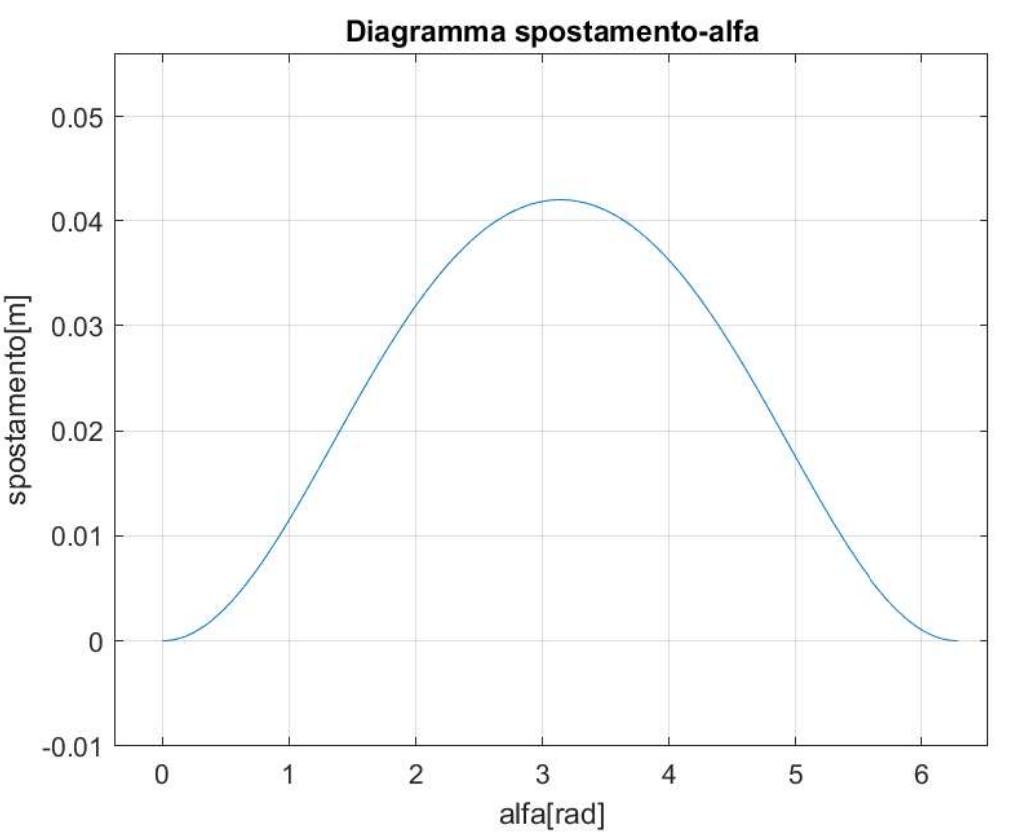
\includegraphics[scale=0.5]{Immagini/GraficoSpostamento.png}
    \caption{Andamento spostamento pistone in dunzione di $\alpha$}
    \label{fig:GraficoSpostamento}
\end{figure}
\begin{lstlisting}[frame=trBL]
%Dati
Ta=293.15;               %Temperatura di aspirazione [K]
k=1.4;                   %Coefficiente isentropica
eps=0.05;                %Coefficiente volume nocivo
Cil=0.0002;              %Cilindrata
Pa=101325;               %Pressione Aspirazione
Pm=1114575;              %Pressione Mandata
r=21*10^-3;              %raggio manovella
l=85*10^-3;              %lunghezza biella
n_cil=2;                 %Numeri cilindri
corsa=0.042;             %corsa cilidri
d=0.055;                 %Alesaggio

%Grandezze Ricavate
Vpmi=Cil*(1+eps);                        %Volume punto morto inferiore
Vpms=Cil*eps;                            %Volume punto morto superiore
lamda=l/r;                               %rapporto biella-manovella
omega=(2*pi*n)/60;                       %Velocita manovella[rad/s]
Vcilindro=(pi*d^2/4)*corsa;              %Cilindrata
Apist=d^2*pi/4;                          %Area pistone

%Grafico spostamento al variare di alfa
alfa=linspace(0,2*pi,6296);      %vettore da 0 a 2pi con 
                                 %6296 volte un radiante
spostamento=r*(1-cos(alfa)+lambda-sqrt(lambda^2-sin(alfa).^2));
plot(alfa,spostamento);
xlabel('alfa[rad]'),ylabel('spostamento[m]'),
        title('Diagramma spostamento-alfa'),
        ylim([ 0.06]),grid on,xlim([0 2*pi]);
\end{lstlisting}
\subsection{Andamento del volume in funzione dell'angolo di manovella}
Considerando quanto ottenuto prima, moltiplicando lo spostamento per la sezione del pistone e aggiungendo il volume nocivo intrappolato a fine compressione, si ottiene l’andamento del volume in funzione dell’angolo di manovella:
\begin{equation}
    V=V_{\mathrm{nocivo}}+s\cdot\frac{\pi d^2}{4}
\end{equation}
\begin{figure}[h]
    \centering
    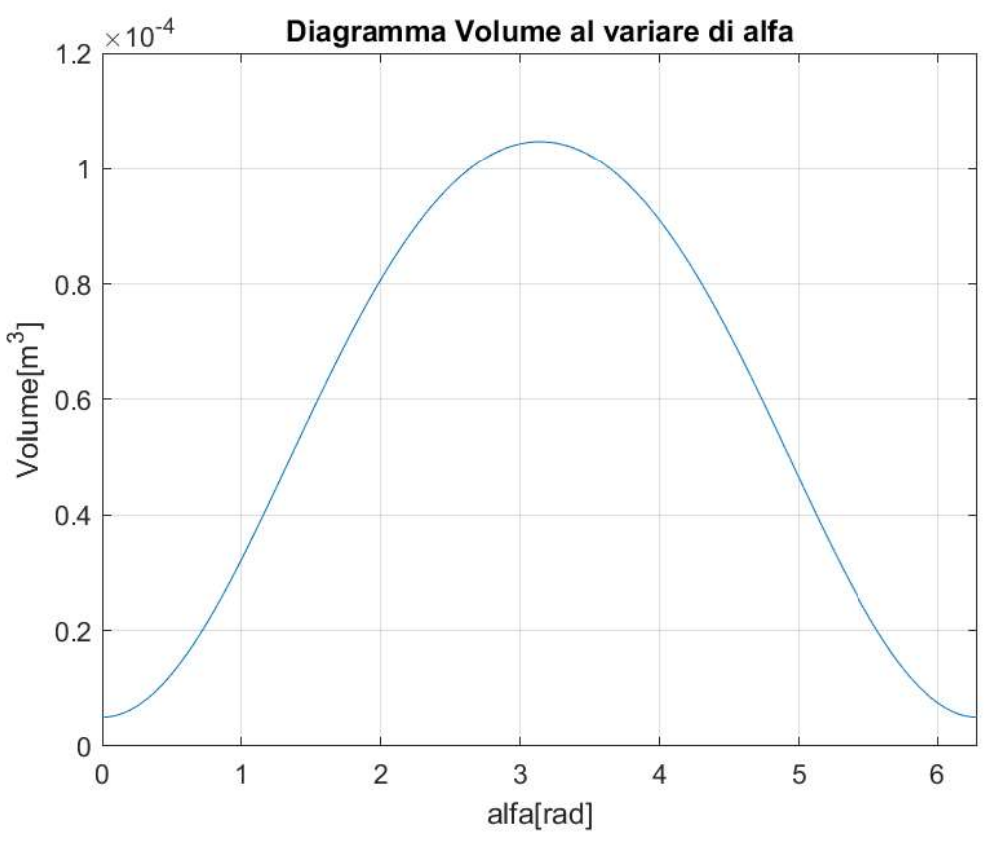
\includegraphics[scale=0.5]{Immagini/GraficoVolume.png}
    \caption{Andamento volume spazzato in funzione di $\alpha$}
    \label{fig:GraficoVolume}
\end{figure}
\begin{lstlisting}[frame=trBL]
%Volume cilindro al variare di alfa%
Vnocivo=eps*Vcilindro;
Vist=Vnocivo+(pi*d^2/4)*spostamento; %volume all'interno di un
                                     %unico cilindro in funzione dello 
                                     %spostamento
plot(alfa,Vist);
xlabel('alfa[rad]'),ylabel('Volume[m^3]'),
      title('Diagramma Volume al variare di alfa'),
      grid on,xlim([0 2*pi]);
\end{lstlisting}
\subsection{Andamento della pressione in funzione dell'angolo di manovella}
Per analizzare l’andamento della pressione all’interno del cilindro, in funzione di $\alpha$, si ipotizza di considerare trasformazioni di compressione ed espansione isoentropiche (nell’ipotesi di aria come gas perfetto).\\
Vale quindi:
\begin{equation}
    pV^k=\mathrm{cost}.
\end{equation}
Questa equazione può essere espressa in funzione di due stati del sistema, uno incognito (pV) ed uno noto ($p_0V_0$).
\begin{equation}
    pV^k=p_0V_0^k.
\end{equation}
Da cui si ricava:
\begin{equation}
    p=p_0\left(\frac{V_0}{V}\right)^k.
\end{equation}
Nel caso di espansione, lo stato noto è lo stato in cui il volume $V_0=V_{\mathrm{nocivo}}$ e quindi la pressione $p_0=p_M$.\\
Si avrà quindi:
\begin{equation}
    p=p_M\left(\frac{V_{\mathrm{nocivo}}}{V}\right)^k
\end{equation}
Nel caso di compressione, invece, lo stato noto sarà quello in cui la pressione $p_0=p_A$ e il volume sarà il volume massimo all’interno del cilindro
$V_0=V_{\mathrm{nocivo}}+V_{\mathrm{cilindro}}$.\\
Per cui:
\begin{equation}
    p=p_A\left(\frac{V_{\mathrm{nocivo}}+V_{\mathrm{cilindro}}}{V}\right)^k
\end{equation}
Avendo precedentemente ricavato l’andamento del volume in funzione dell’angolo di manovella, sempre in ambiente Matlab è stato possibile ottenere il grafico rappresentante la pressione in funzione del medesimo angolo.\\
\begin{figure}[h!]
    \centering
    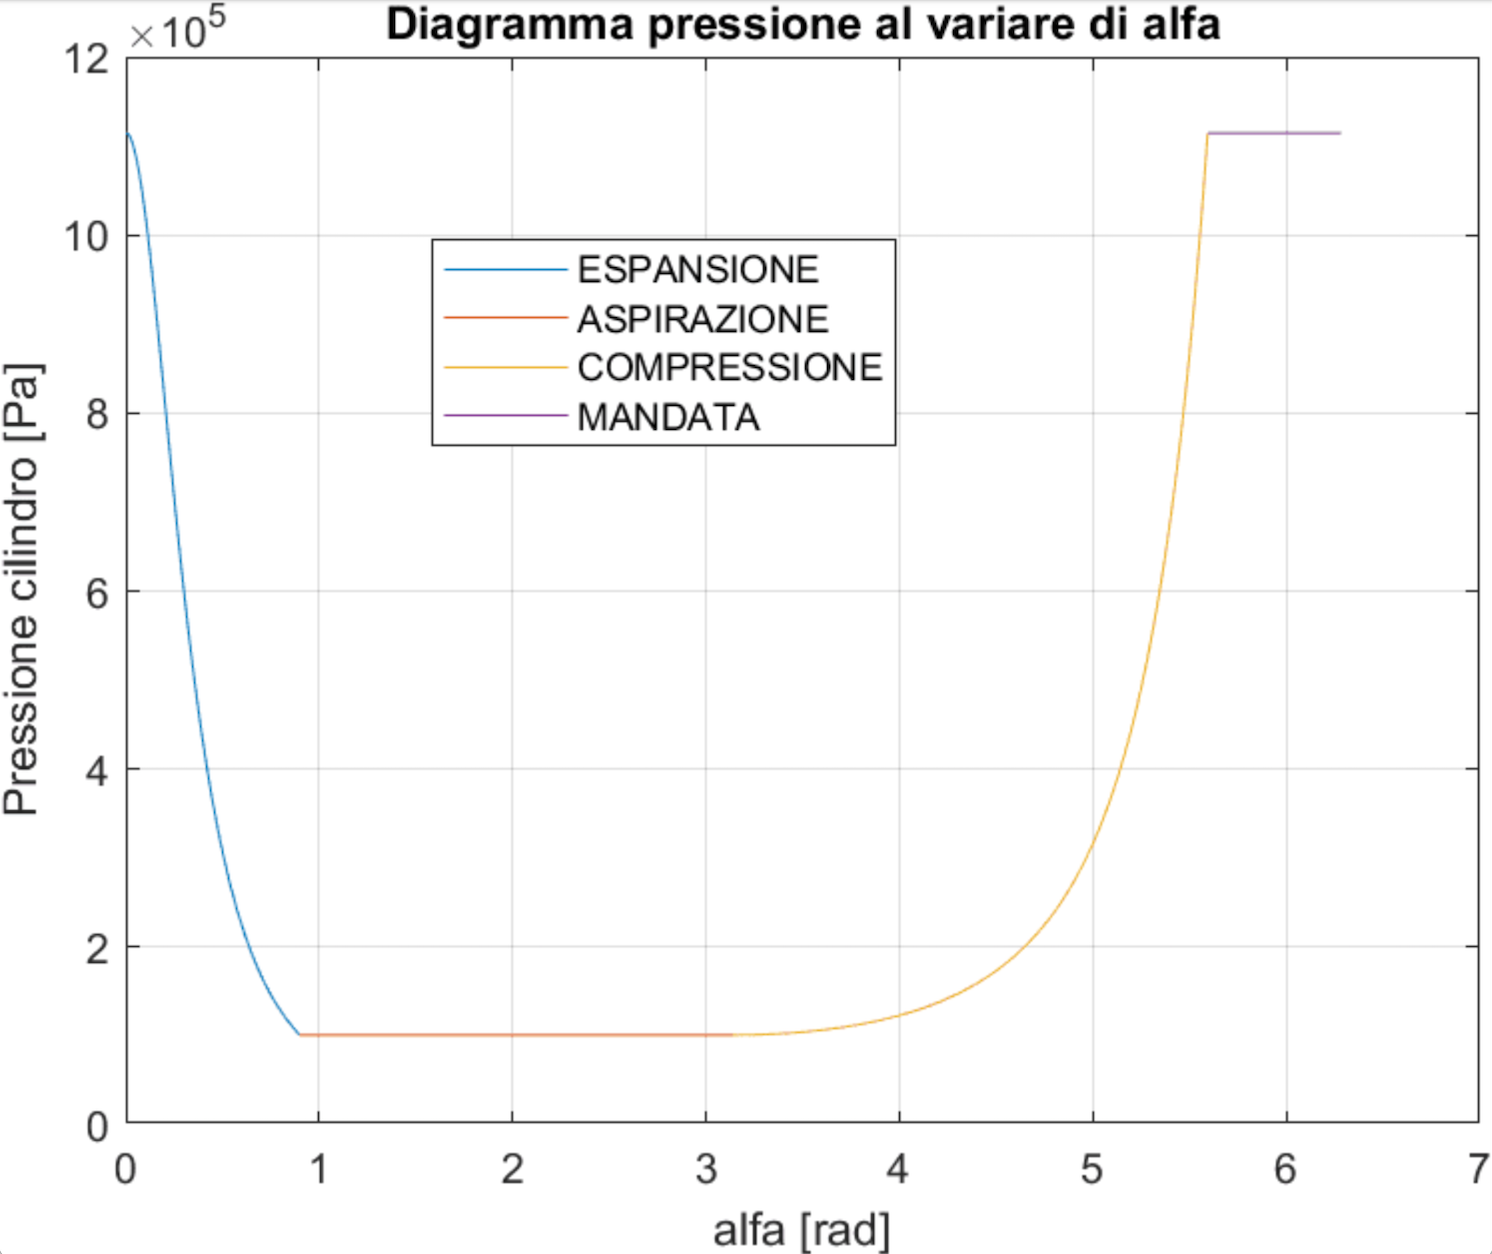
\includegraphics[scale=0.35]{Immagini/GraficoPressione.png}
    \caption{Andamento della pressione in funzione di $\alpha$}
    \label{fig:GraficoPressione}
\end{figure}
\begin{lstlisting}[frame=trBL]
%grafico pressione al variare di alfa

%espansione
alfaesp=linspace(0,0.8989, )
spostamentoesp=r*(1-cos(alfaesp)+lambda-
               sqrt(lambda^2-sin(alfaesp).^2))
Vistesp=Vnocivo+(pi*d^2/4)*spostamentoesp
pressioneesp=Pm*(Vnocivo*((Vistesp).^-1)).^k;
plot(alfaesp,pressioneesp);
hold on

%aspirazione
ya=Pa*ones(1,737);
xa=linspace(0.8989,pi,2000);
plot(x,y);
hold on

%compressione
alfacomp=linspace(pi,5.5934,758)
spostamentocomp=r*(1-cos(alfacomp)+lambda-
                sqrt(lambda^2-sin(alfacomp).^2))
Vistcomp=Vnocivo+(pi*d^2/4)*spostamentocomp
pressionecomp=Pa*((Vnocivo+Vcilindro)*((Vistcomp).^-1)).^k;
plot(alfacomp,pressionecomp)
hold on

%mandata
ym=Pm*ones(1,241);
xm=linspace(5.5934,2*pi,2000);
plot(x,y);
hold on
grid on
xlabel('alfa [rad]'),ylabel('Pressione cilindro [Pa]'),
      title('Diagramma pressione al variare di alfa');
\end{lstlisting}
\newpage
\subsection{Valutazione della massa dei componenti}
Per procedere con l'analisi dei carichi è indispensabile determinare le masse dei principali elementi del cinematismo. Queste possono essere valutate modellando i componenti con un programma di disegno solido (SOLIDWORKS nel nostro caso).
Una volta definita la geometria del pezzo, la funzione "proprietà di massa" permetterà di determinare le grandezze caratteristiche
\subsubsection{Pistone}
\begin{figure}[h]
    \centering
    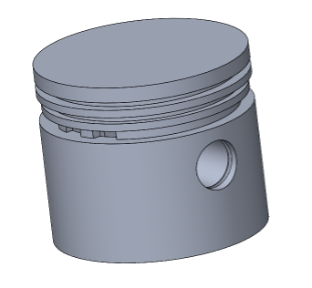
\includegraphics[scale=0.8]{Immagini/PistoneCAD.png}
    \caption{Modello CAD SOLIDWORKS del pistone}
    \label{fig:PistoneCAD}
\end{figure}
\begin{figure}[h]
    \centering
    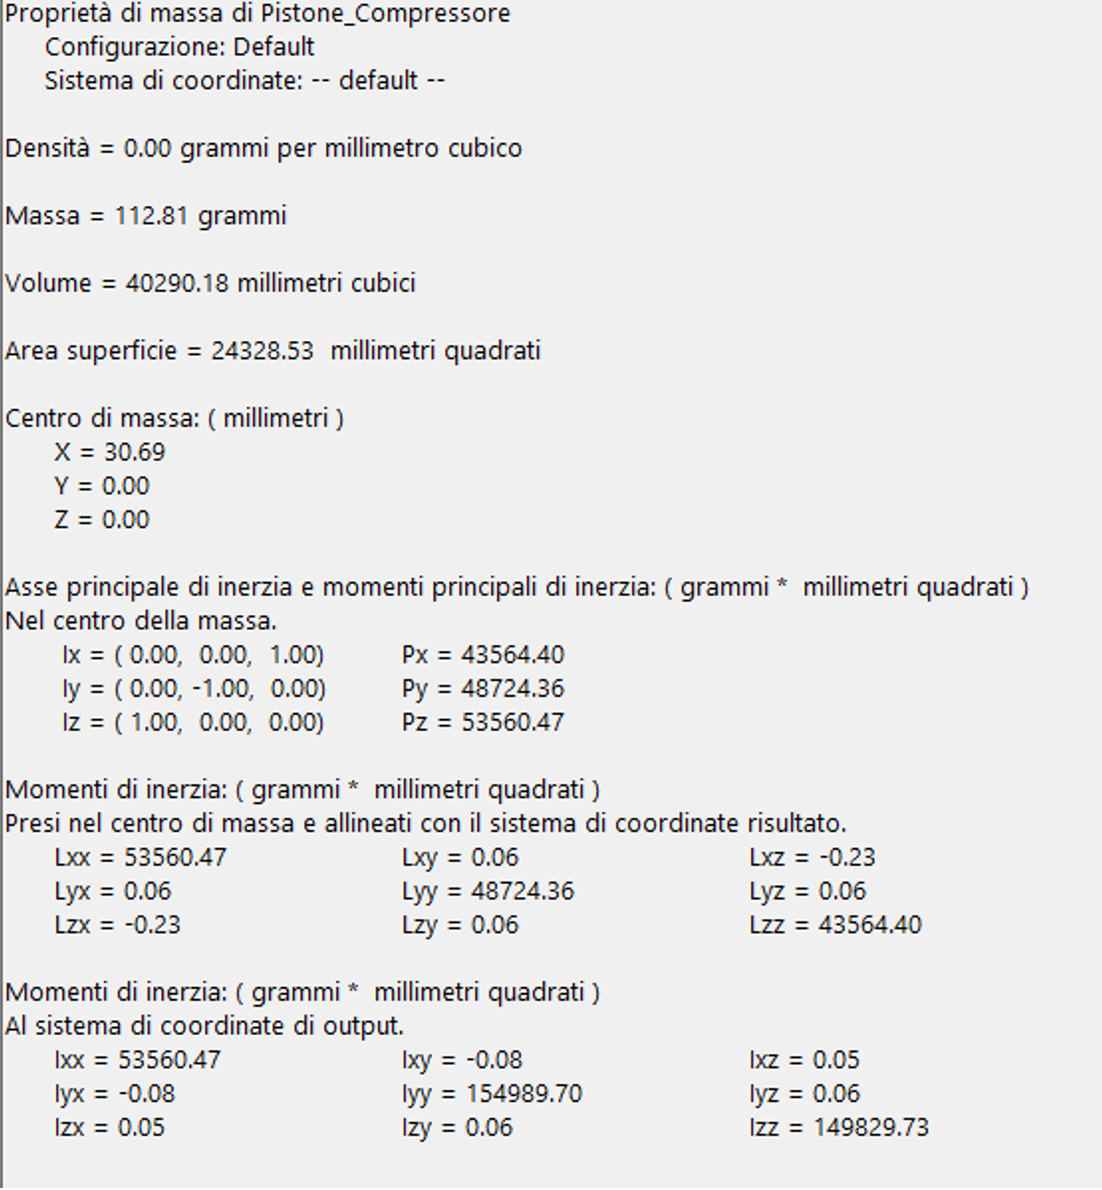
\includegraphics[scale=0.47]{Immagini/CaratteristichePistone.png}
    \caption{Caratteristiche pistone ricavate mediante sofrtware SOLIDWORKS}
    \label{fig:Pistone}
\end{figure}
\newpage
\subsubsection{Biella}
\begin{figure}[h]
\centering
   {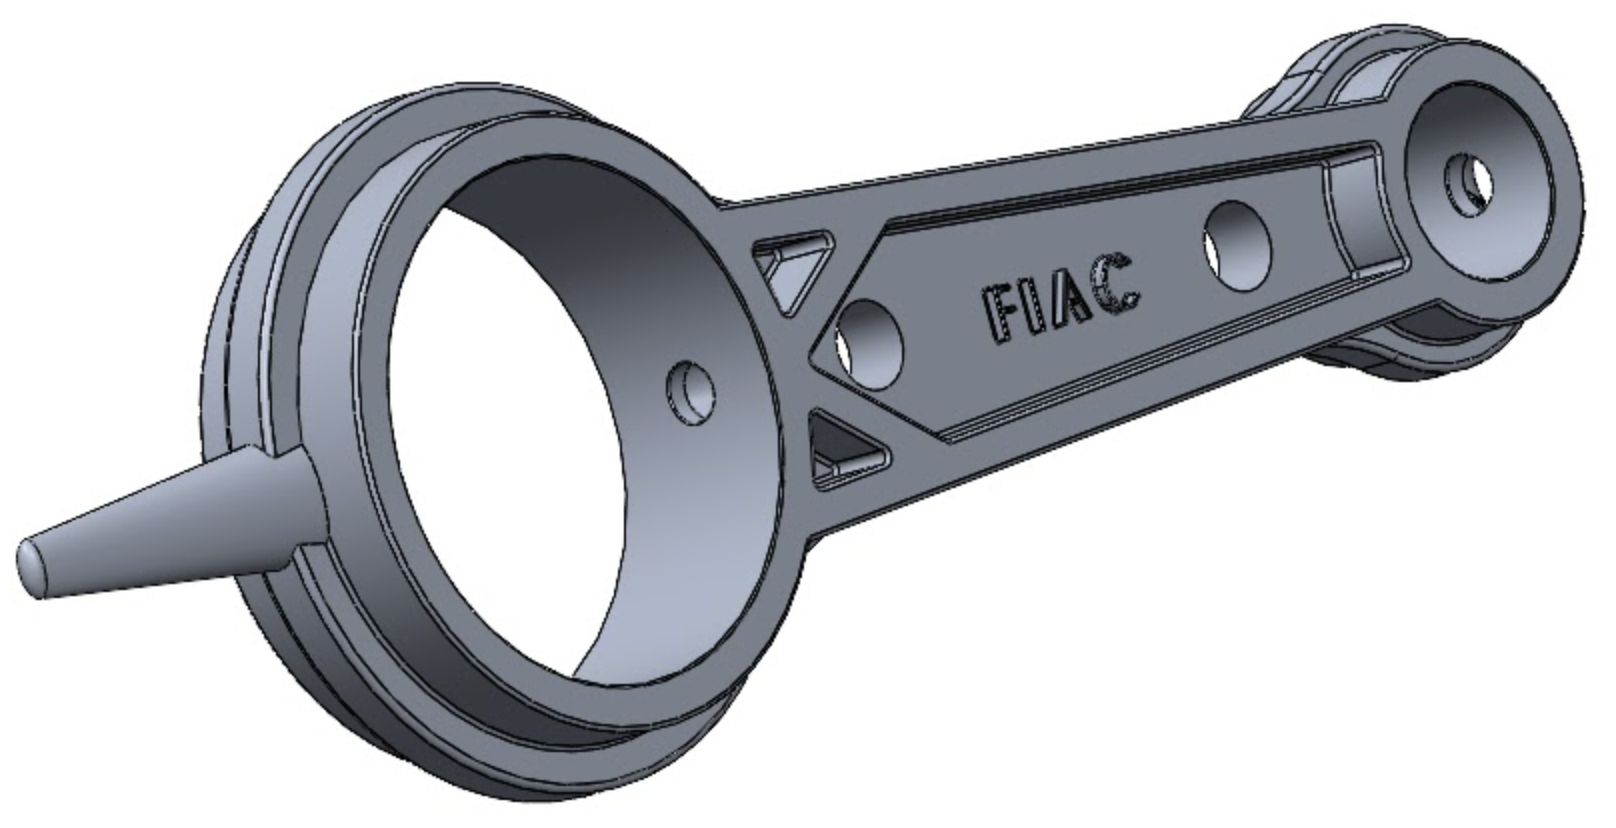
\includegraphics[width=.46\textwidth]{Immagini/Biella1.png}} \quad
   {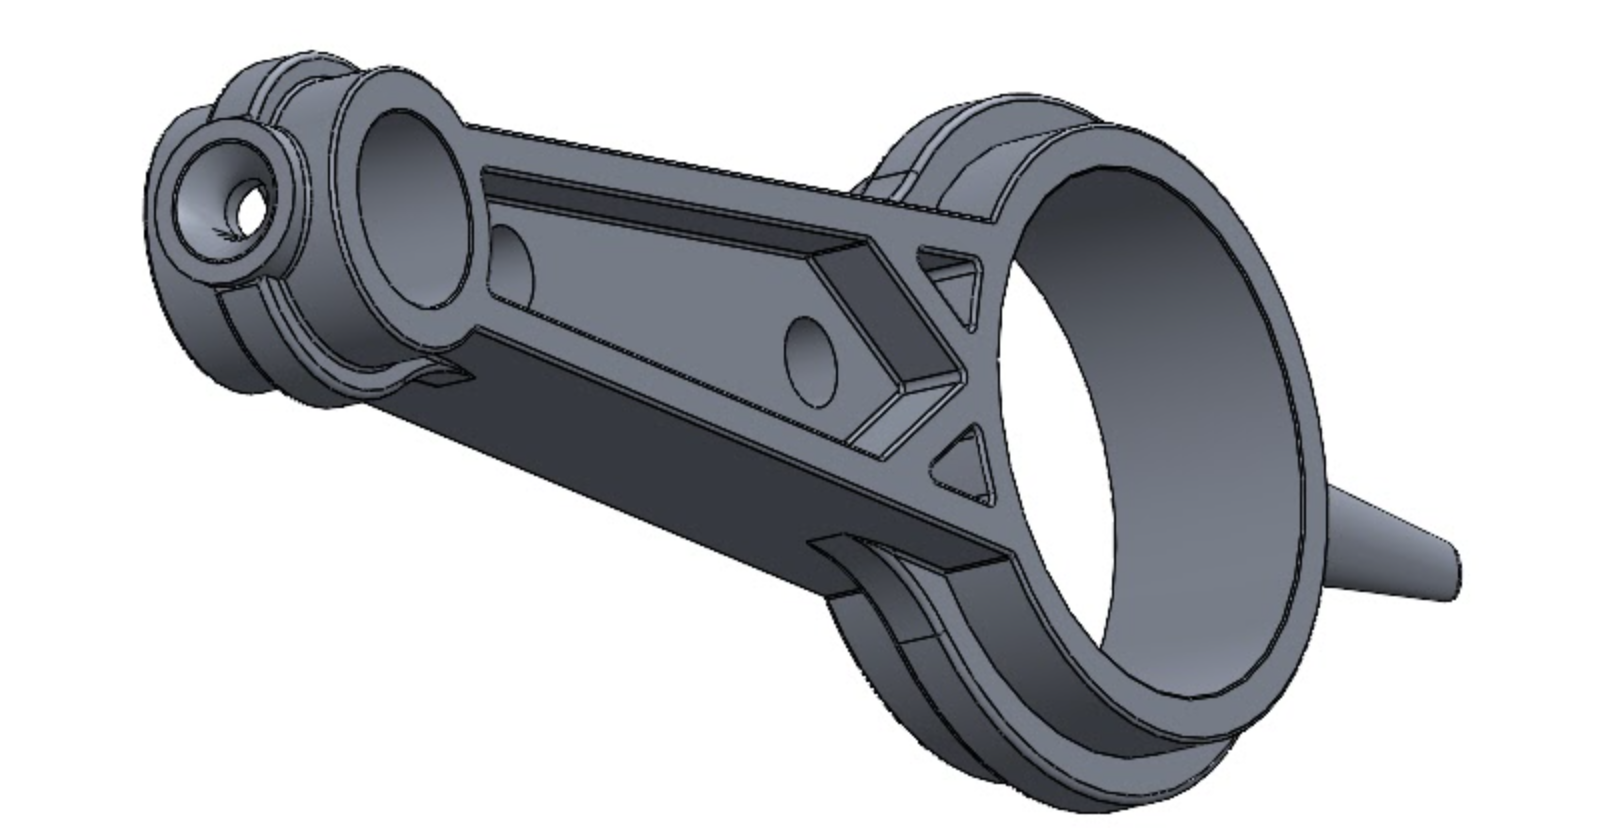
\includegraphics[width=.49\textwidth]{Immagini/Biella2.png}}
\caption{Modello CAD SOLIDWORKS della biella}
\label{fig:Biella}
\end{figure}
\begin{figure}[h]
    \centering
    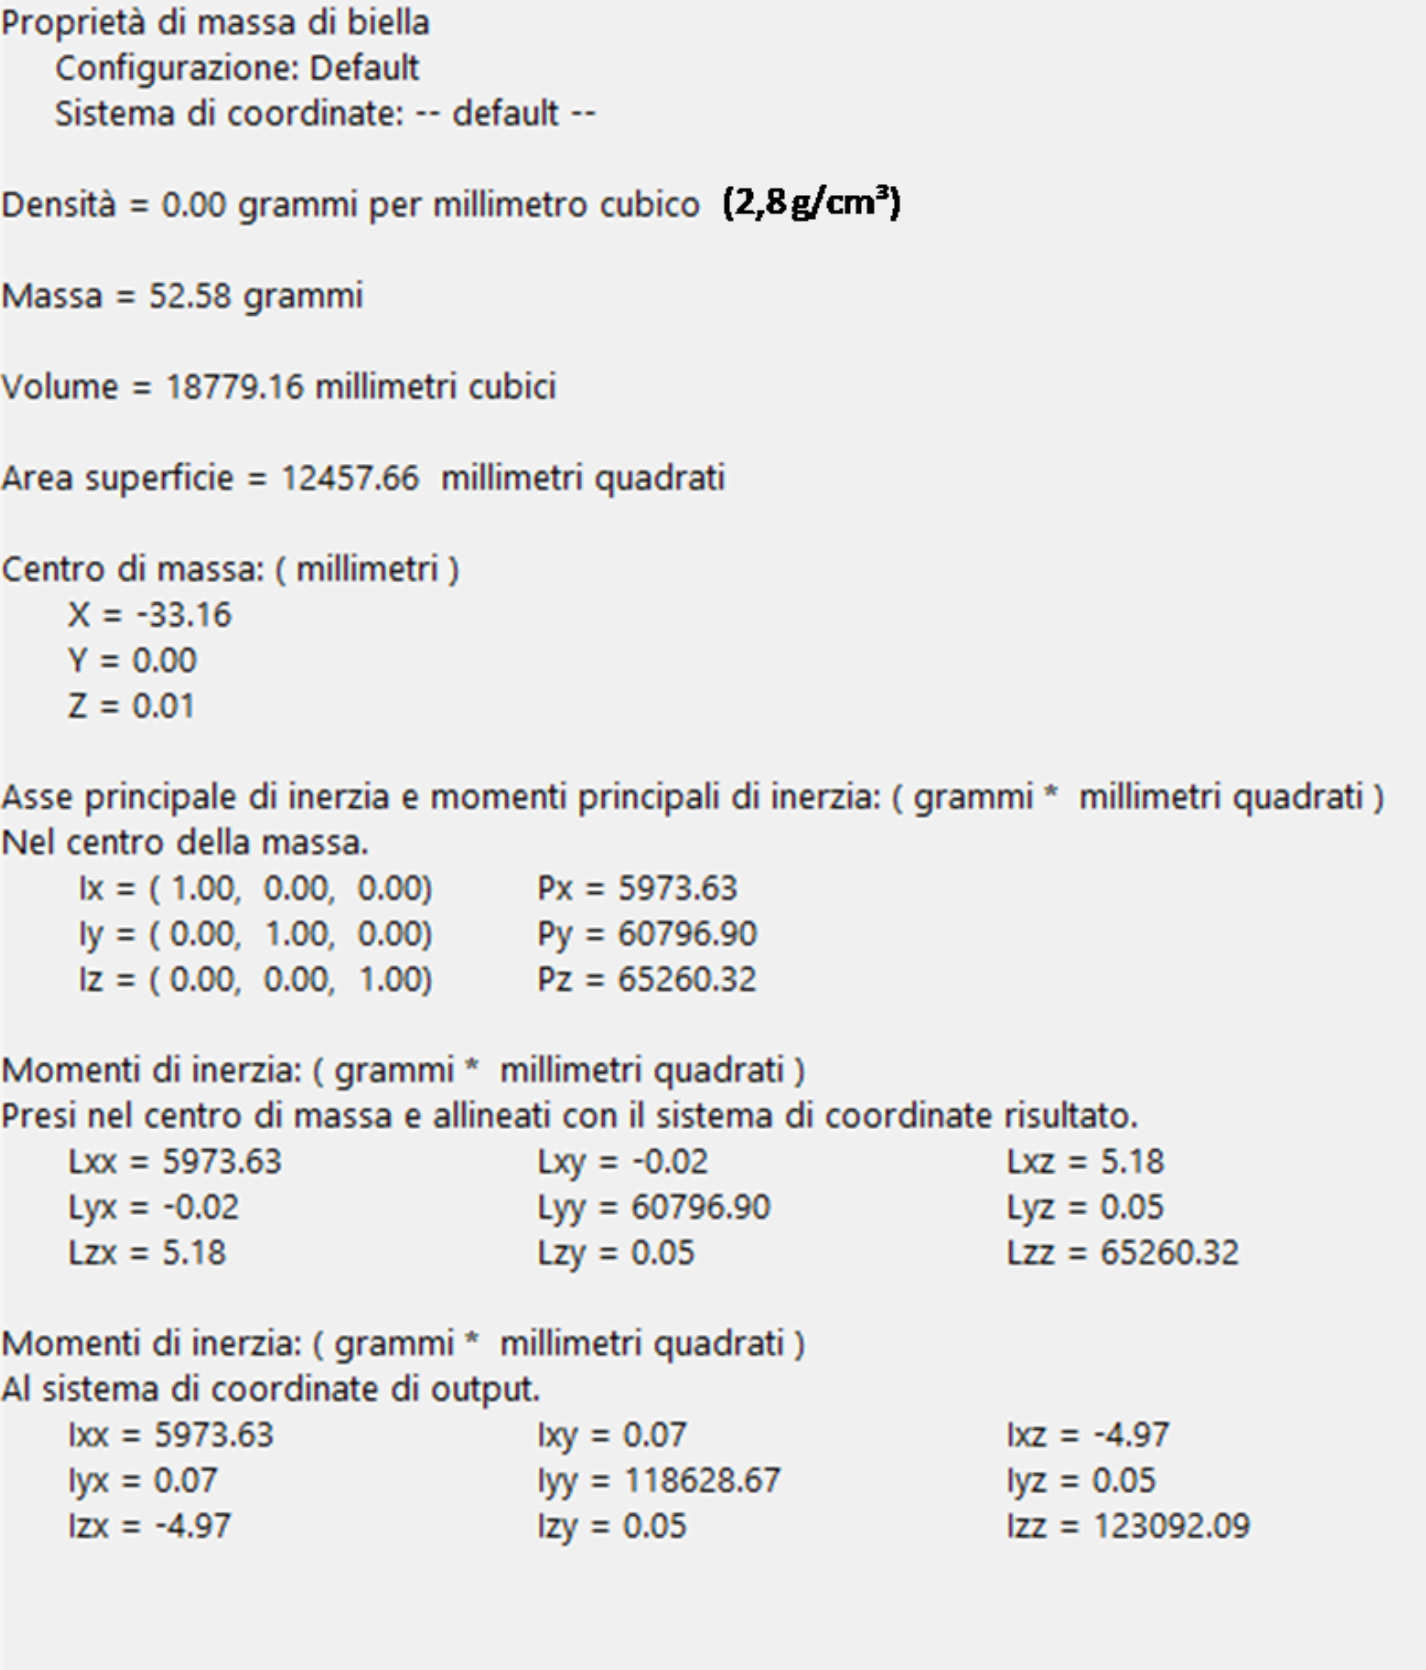
\includegraphics[scale=0.4]{Immagini/CaratteristicheBiella.png}
    \caption{Caratterstiche biella ricavate mediante software SOLIDWORKS}
    \label{fig:CaratteristicheBiella}
\end{figure}
\newpage
\subsubsection{Spinotto}
\begin{figure}[h]
\centering
   {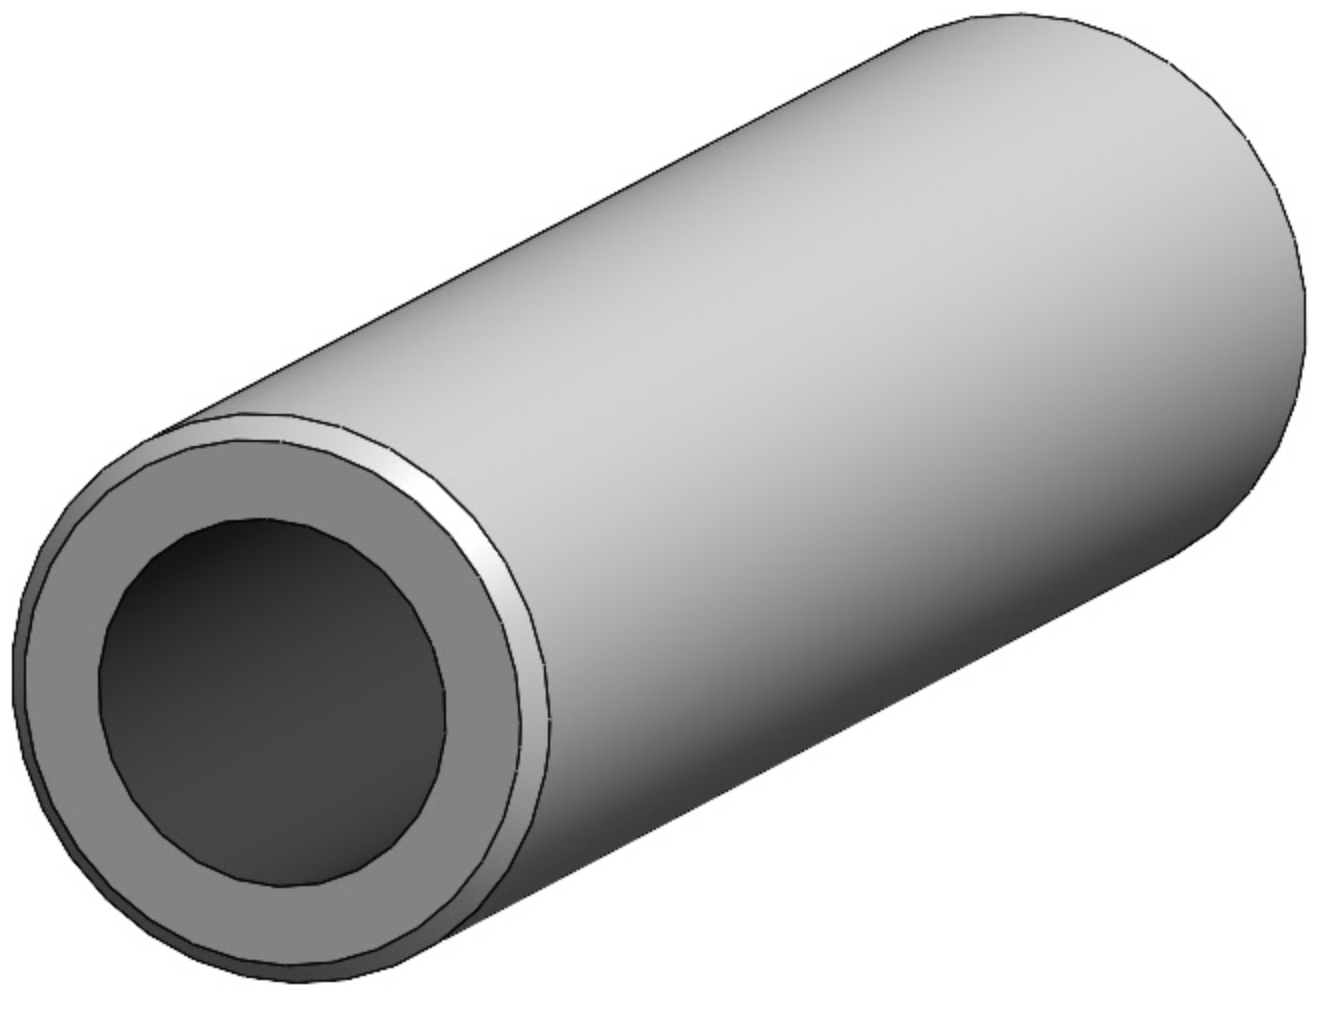
\includegraphics[width=.35\textwidth]{Immagini/Spinotto1.png}} \quad
   {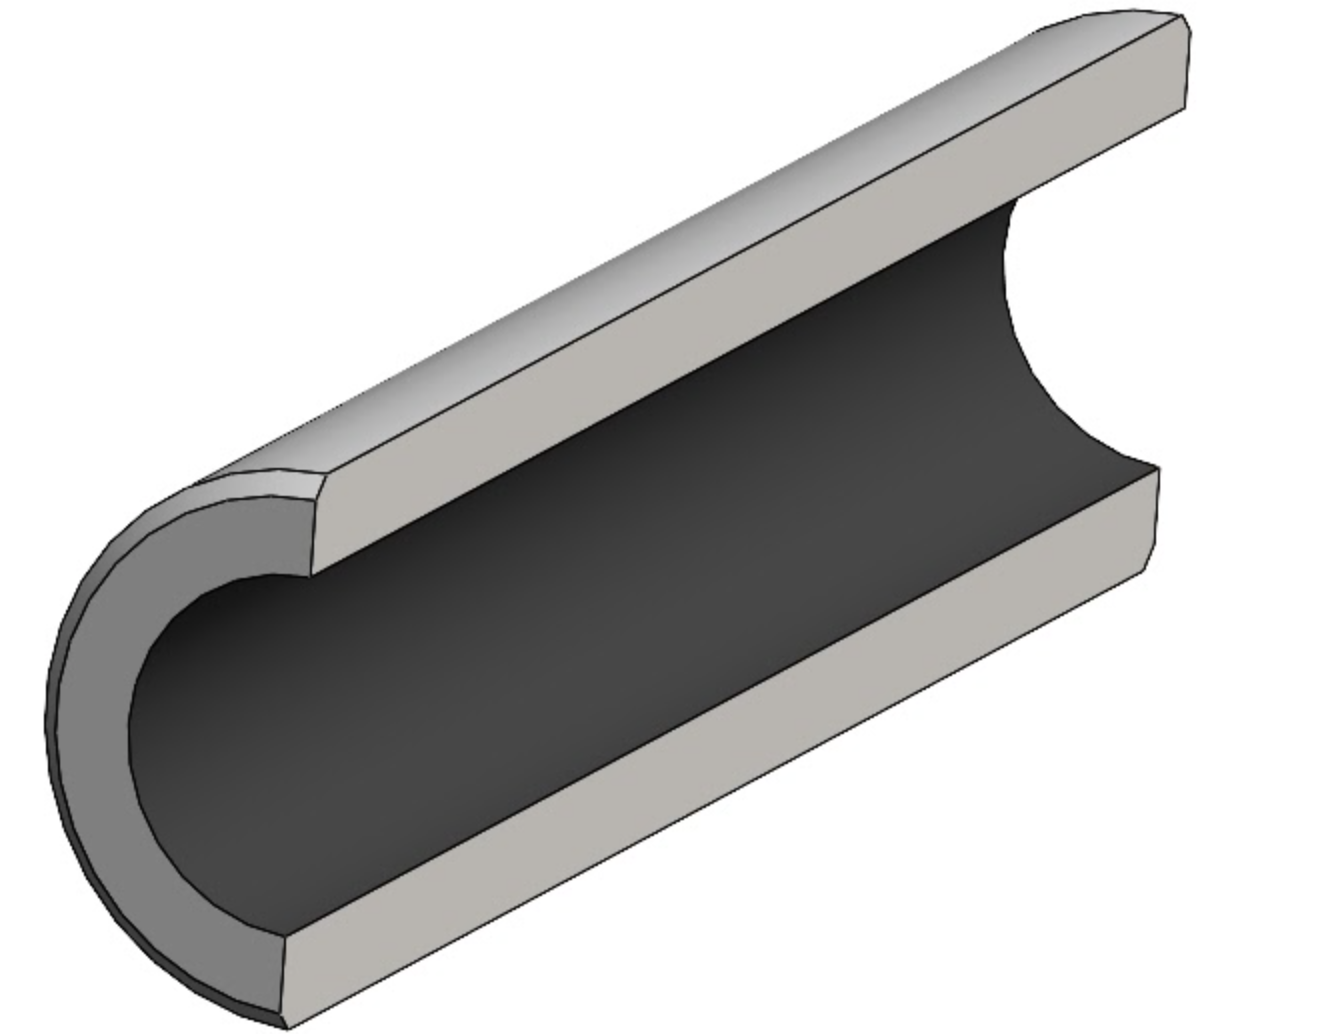
\includegraphics[width=.35\textwidth]{Immagini/Spinotto2.png}}
\caption{Modello CAD SOLIDWORKS dello spinotto}
\label{fig:Spinotto}
\end{figure}
\begin{figure}[h]
    \centering
    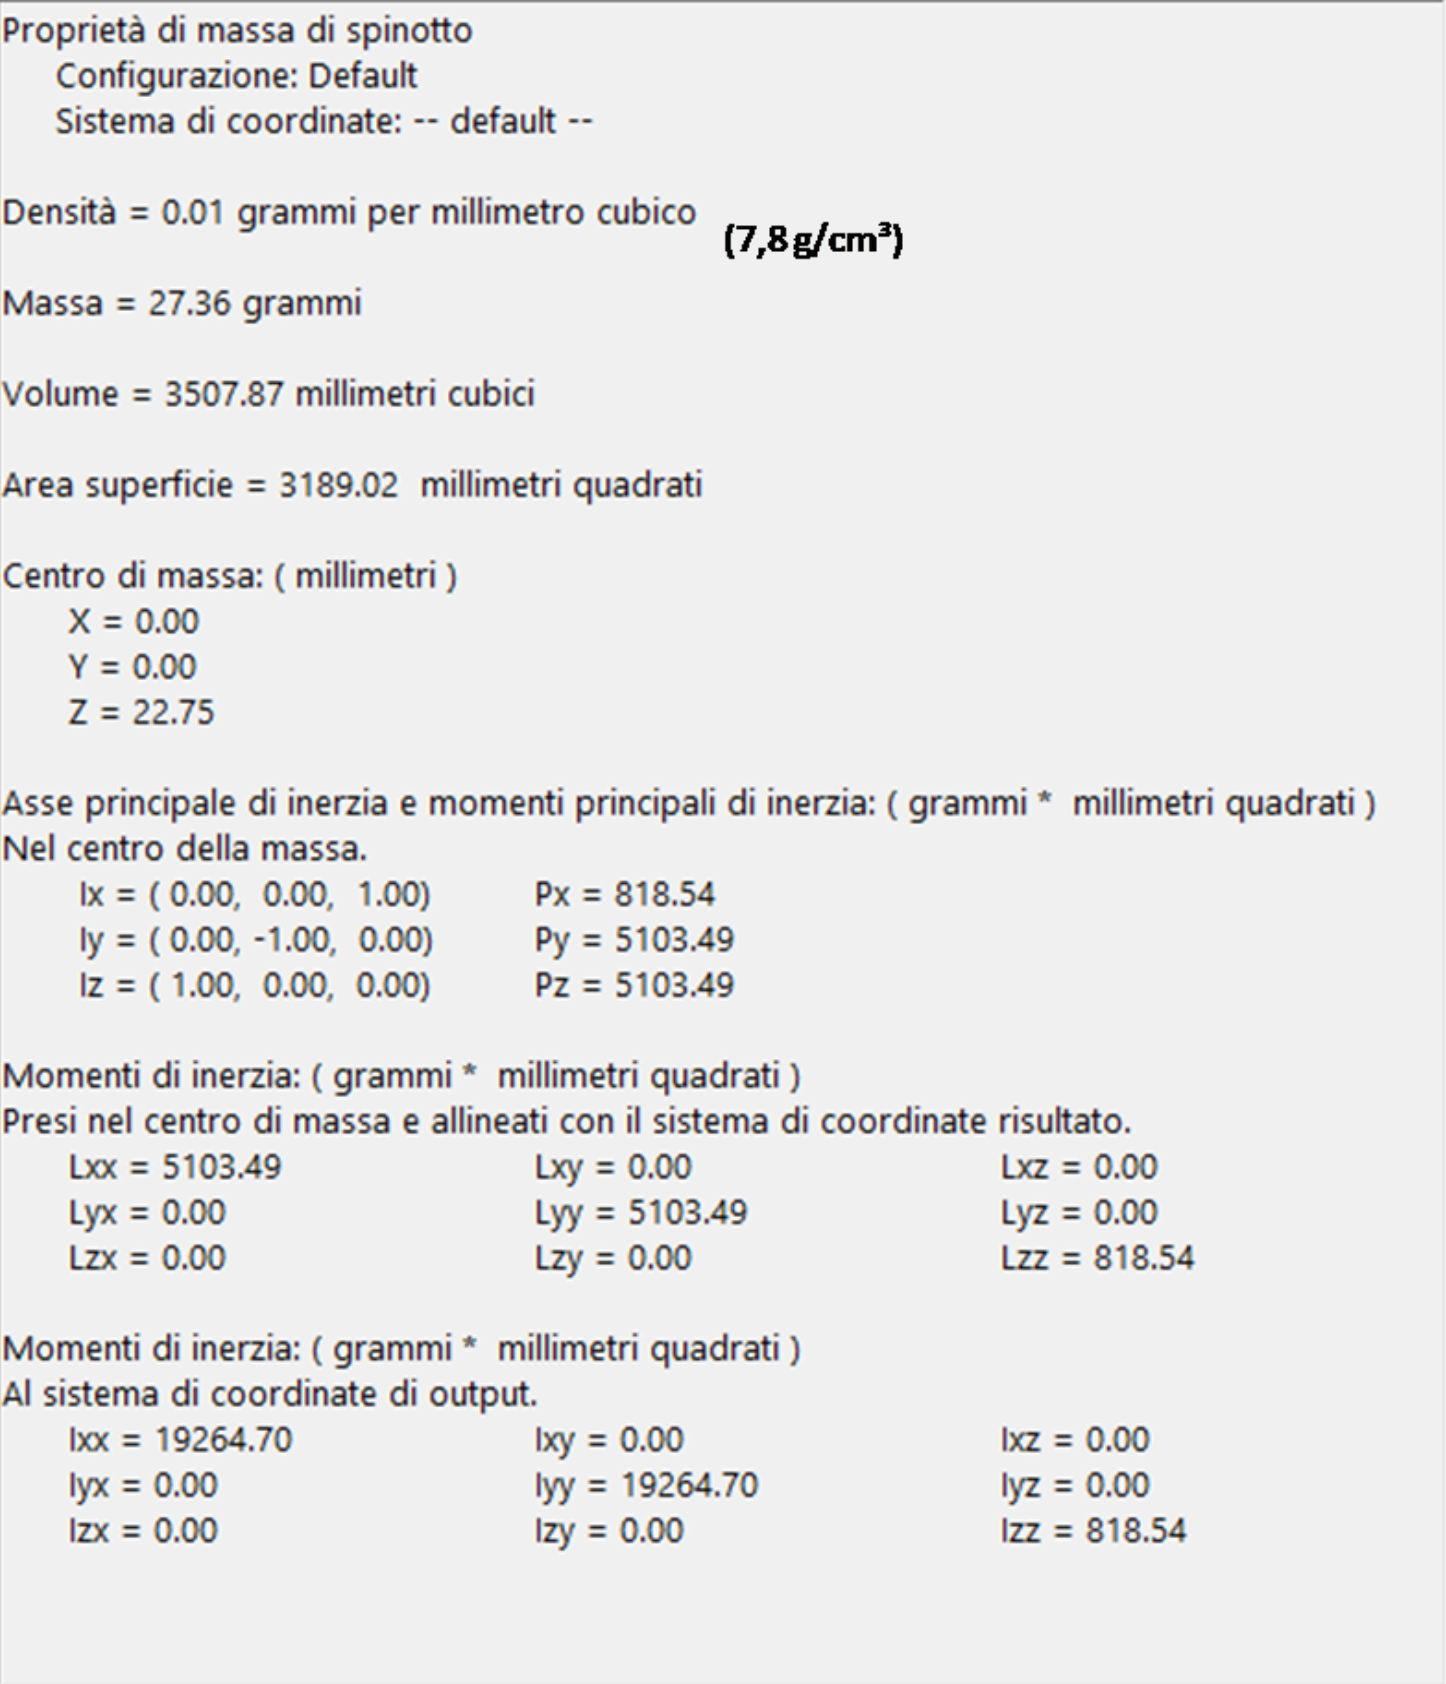
\includegraphics[scale=0.37]{Immagini/CaratteristicheSpinotto.png}
    \caption{Caratteristiche dello spinotto ricavate mediante software SOLIDWORKS}
    \label{fig:CaratteristicheSpinotto}
\end{figure}
\newpage
\subsubsection{Albero a gomiti}
\begin{figure}[h]
\centering
   {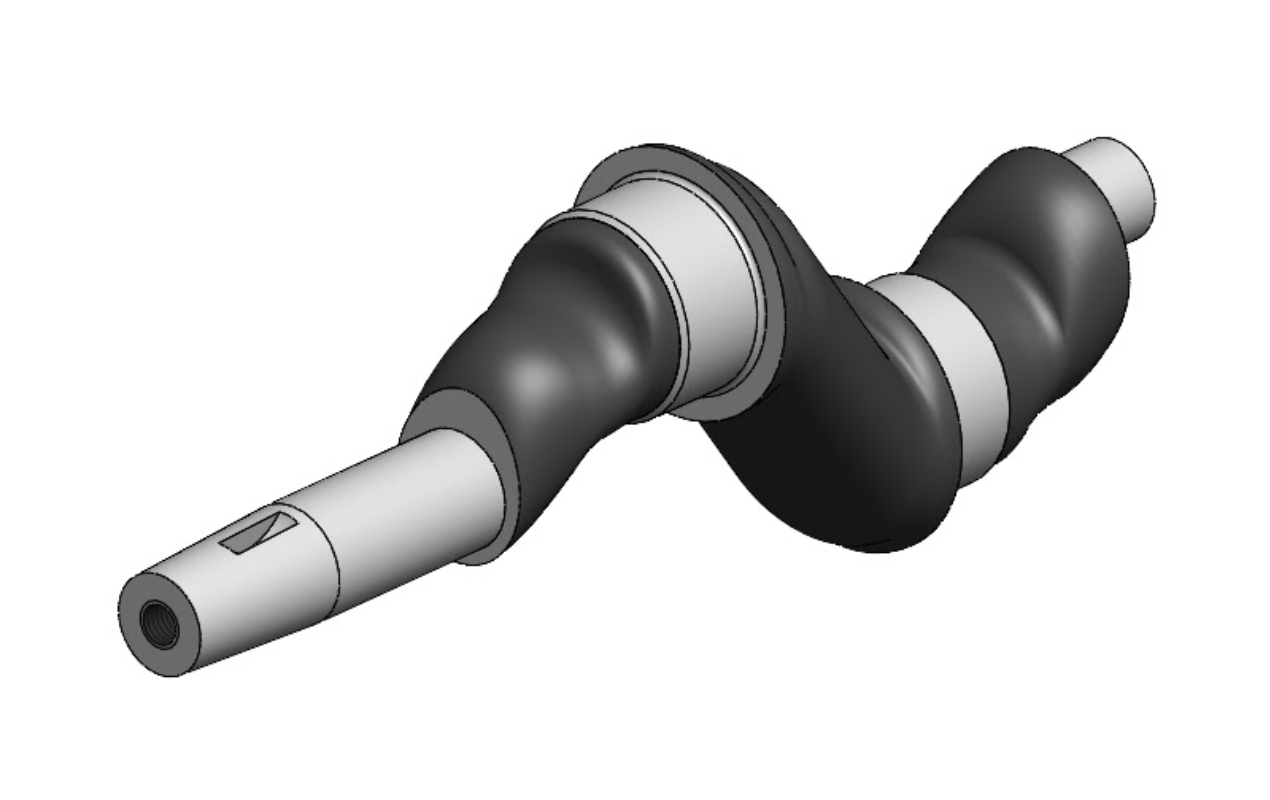
\includegraphics[width=.48\textwidth]{Immagini/Albero1.png}} \quad
   {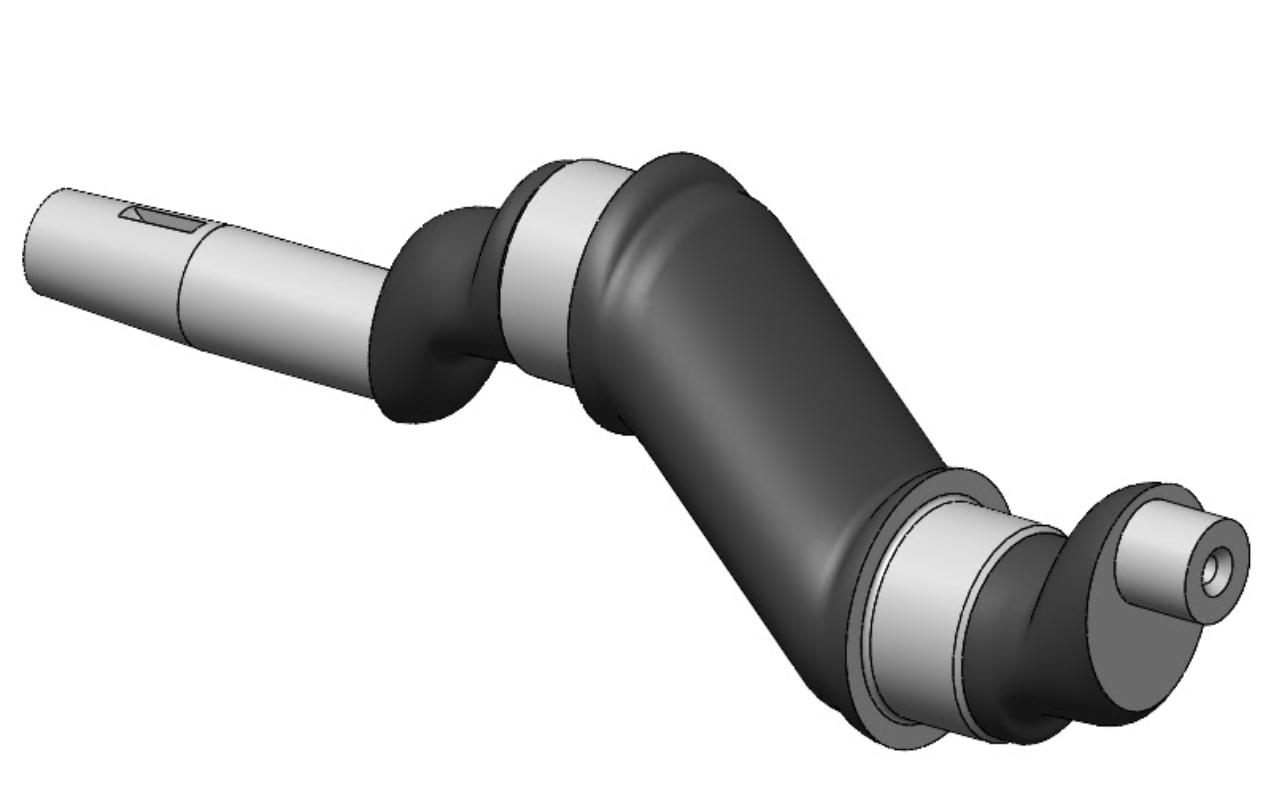
\includegraphics[width=.48\textwidth]{Immagini/Albero2.png}}
\caption{Modello CAD SOLIDWORKS dell'albero}
\label{fig:Albero}
\end{figure}
\begin{figure}[h]
    \centering
    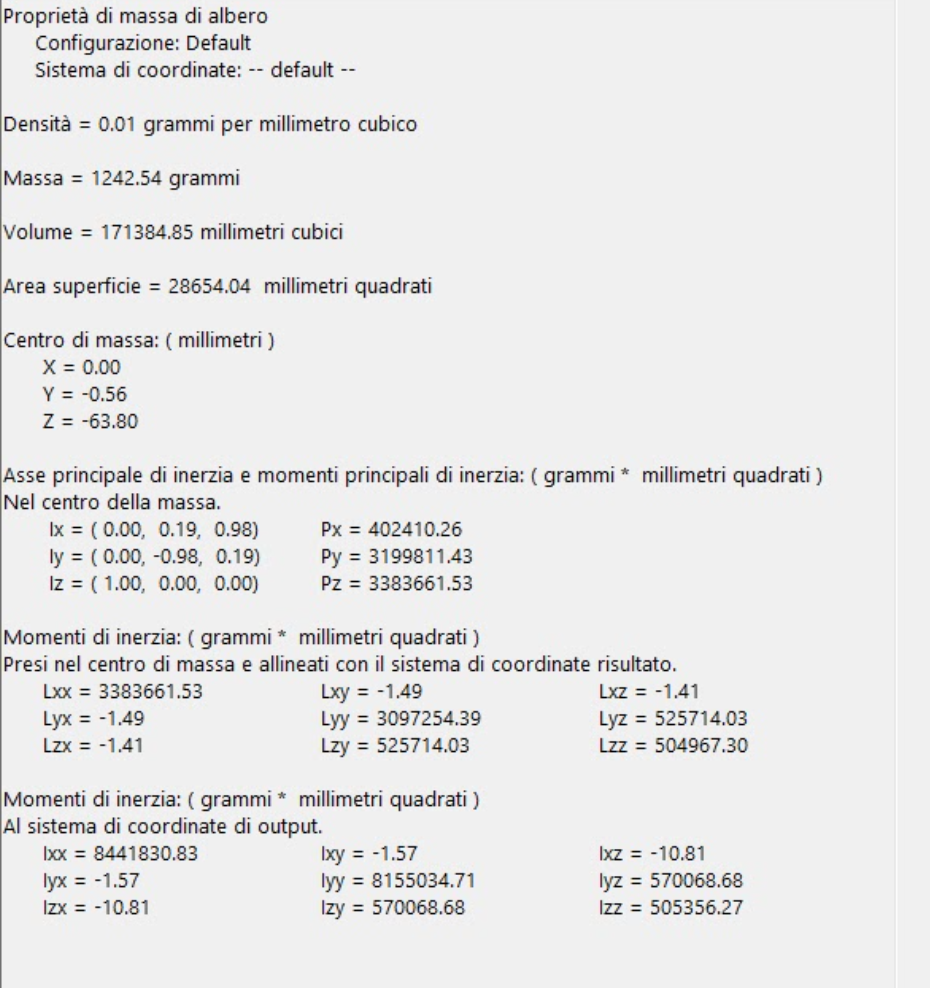
\includegraphics[scale=0.66]{Immagini/CaratteristicheAlbero.png}
    \caption{Caratteristiche dell'albero ricavate mediante software SOLIDWORKS}
    \label{fig:CaratteristicheAlbero}
\end{figure}
\newpage
\subsection{Andamento delle forze agenti in funzione dell'angolo di manovella}
Si analizzano ora le forze agenti sui vari elementi del cinematismo biella, pistone, spinotto e albero motore dovute all’effetto della pressione e alle azioni inerziali. 
\subsubsection{Pistone}
La forza complessiva che agisce sul pistone è data dalla somma del contributo dovuto alla pressione del fluido e quello dovuto all’inerzia dei corpi.
\paragraph{Forza dovuta alla pressione del fluido}
In questo caso il riferimento all’interno del quale la forza è stata calcolata è relativo, perché la sollecitazione è quella che agisce sul pistone; quindi, il punto di vista è all’interno del cilindro.\\
Per questo motivo la pressione istante per istante viene diminuita della pressione atmosferica. 
\begin{figure}[h]
    \centering
    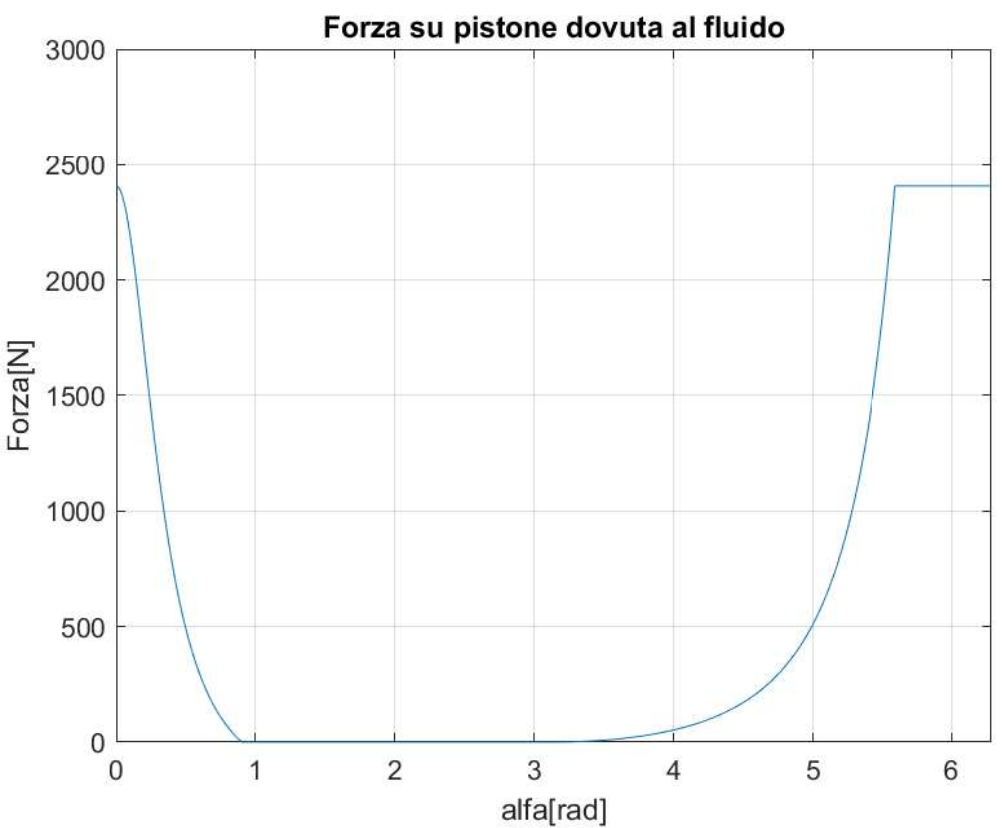
\includegraphics[scale=0.6]{Immagini/ForzaFluidoPistone.png}
    \caption{Forza esercitata dalla pressione del fluido sul pistone in funzione di $\alpha$}
    \label{fig:ForzaFluidoPistone}
\end{figure}
\begin{lstlisting}[frame=trBL]
%Calcolo forza su pistone%

Pressione=[ pressioneesp ya pressionecomp ym];  %raccolgo tutti i 
                                               %valori delle pressioni 
                                                %al variare degli 
                                                %angoli, per poi 
                                                %sottrarci 101325 Pa
alfatot=[ alfaesp xa alfacomp xm ]; %vettore degli angoli
Prel=Pressione-101325;
Forzapistone1= Apist*Prel; %1 perche dovuta al fluido
plot(alfatot,Forzapistone1);
xlabel('alfa[rad]'),ylabel('Forza[N]'),
      title('Forza su pistone dovuta al fluido'),
      grid on,xlim([0 2*pi]),ylim([0 3000]);
\end{lstlisting}
\paragraph{Forza dovuta all'inerzia del pistone}Per ricavare la forza dovuta all’inerzia è necessario ricavare l’accelerazione del pistone in funzione dell’angolo di manovella.\\
\\
Derivando due volte la formula dello spostamento in funzione del tempo (eq.(\ref{spostamento})) è possibile ricavare l’accelerazione cercata:
\begin{equation}
    a=\frac{dv}{dt}=\frac{d^2s}{{dt}^2}=\omega^2r(cos(\alpha)+\frac{cos(2\alpha)}{\lambda})
\end{equation}
con $\omega=\frac{2\pi n}{60}$.
\\
L'andamento dell'accelerazione in funzione dell'angolo di manovella è stato ricavato in ambiente Matlab.
\begin{figure}[h]
    \centering
    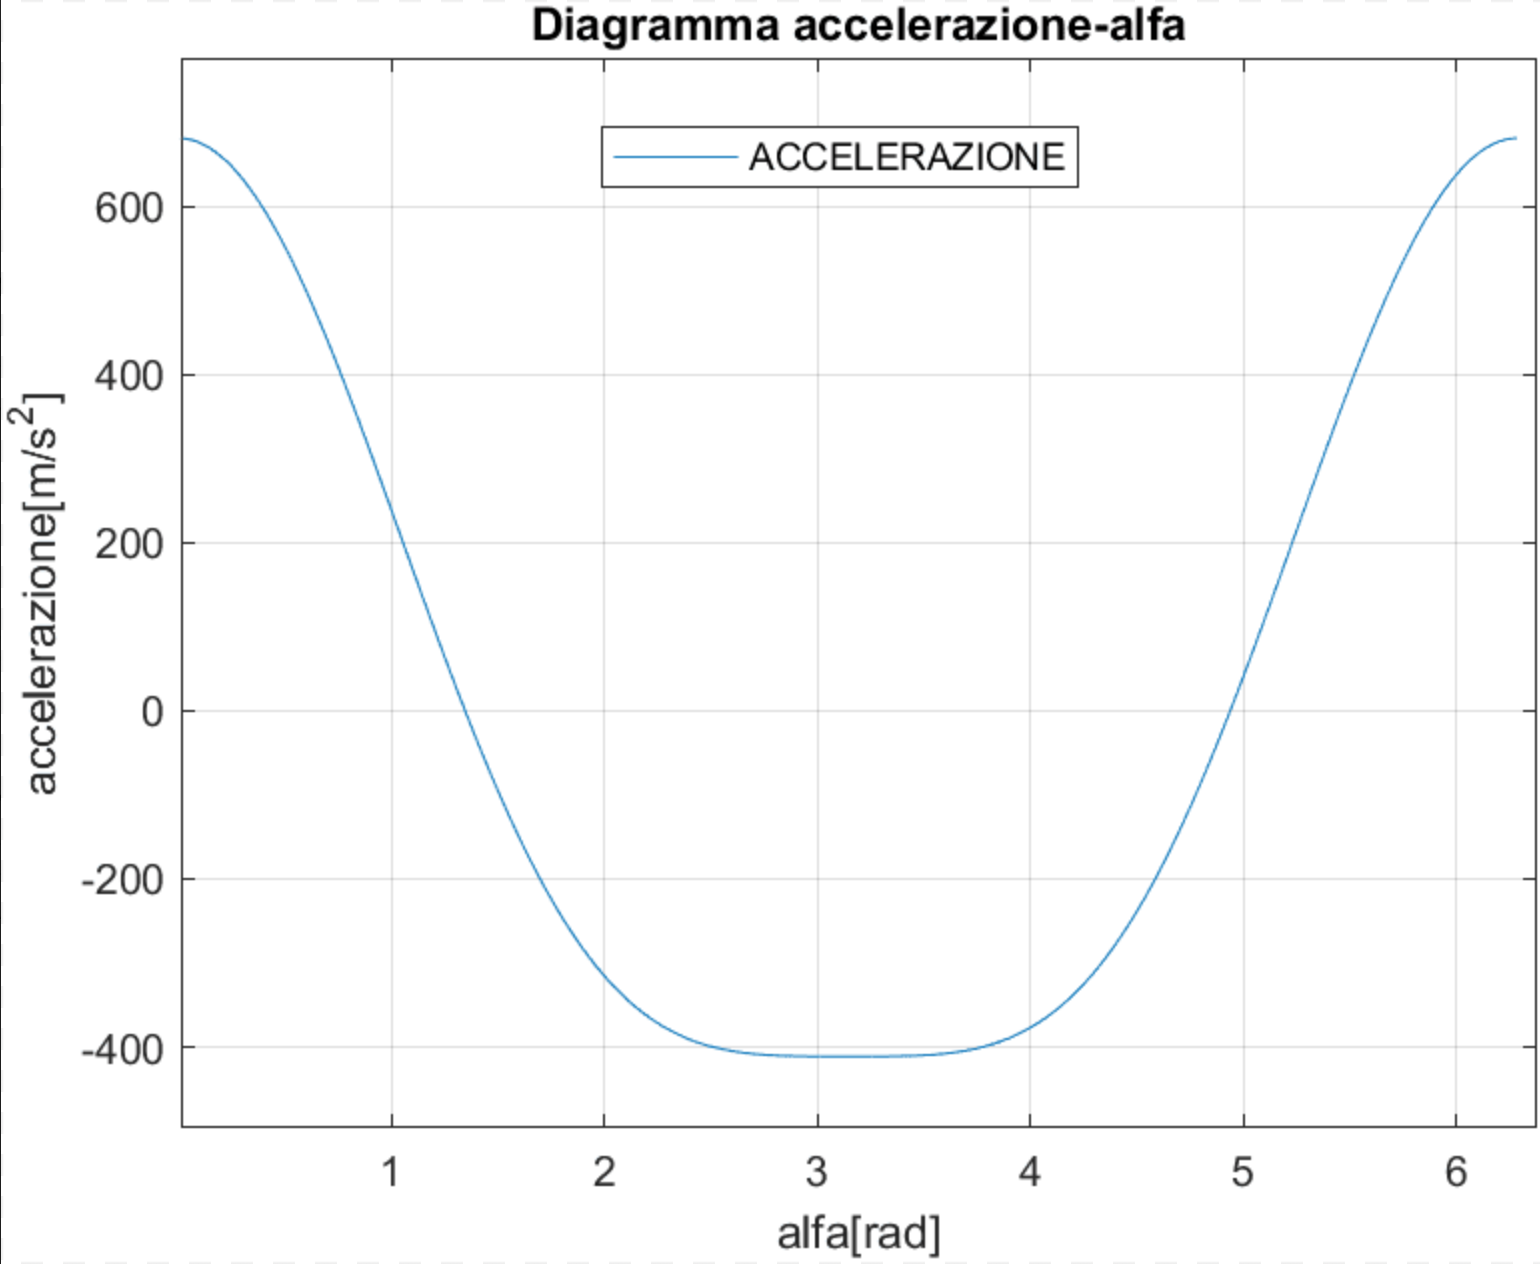
\includegraphics[scale=0.35]{Immagini/GraficoAccelerazionePistone.png}
    \caption{Accelerazione pistone in funzione dell'angolo di manovella}
    \label{fig:GraficoAccelerazionePistone}
\end{figure}
\begin{lstlisting}[frame=trBL]
%Grafico accelerazione al variare di alfa

alfa=linspace(0,2*pi,2000)
accelerazione=(w^2)*r*((cos(alfa))+(cos(2*alfa)*lambda^(-1)));
plot(alfa,accelerazione);
xlabel('alfa[rad]'),ylabel('accelerazione[m/s^2]'),
      title('Diagramma accelerazione-alfa'),grid on;xlim(0,2*pi);
\end{lstlisting}
\newpage
La forza di inerzia si definisce come:
\begin{equation}
    F_i=-m_{pistone}\cdot a_{pistone}
\end{equation}
Questa forza ha una direzione parallela a quella del moto del pistone e con verso discorde a quello dell’accelerazione.\\
La massa del pistone è stata determinata precedentemente mediante software di modellazione SOLIDWORKS ($m_p$=112,81 g).\\
Anche in questo caso è stato ricavato l'andamento mediante uno script Matlab dell'andamento di questa forza in funzione dell'angolo di manovella.
\begin{figure}[h]
    \centering
    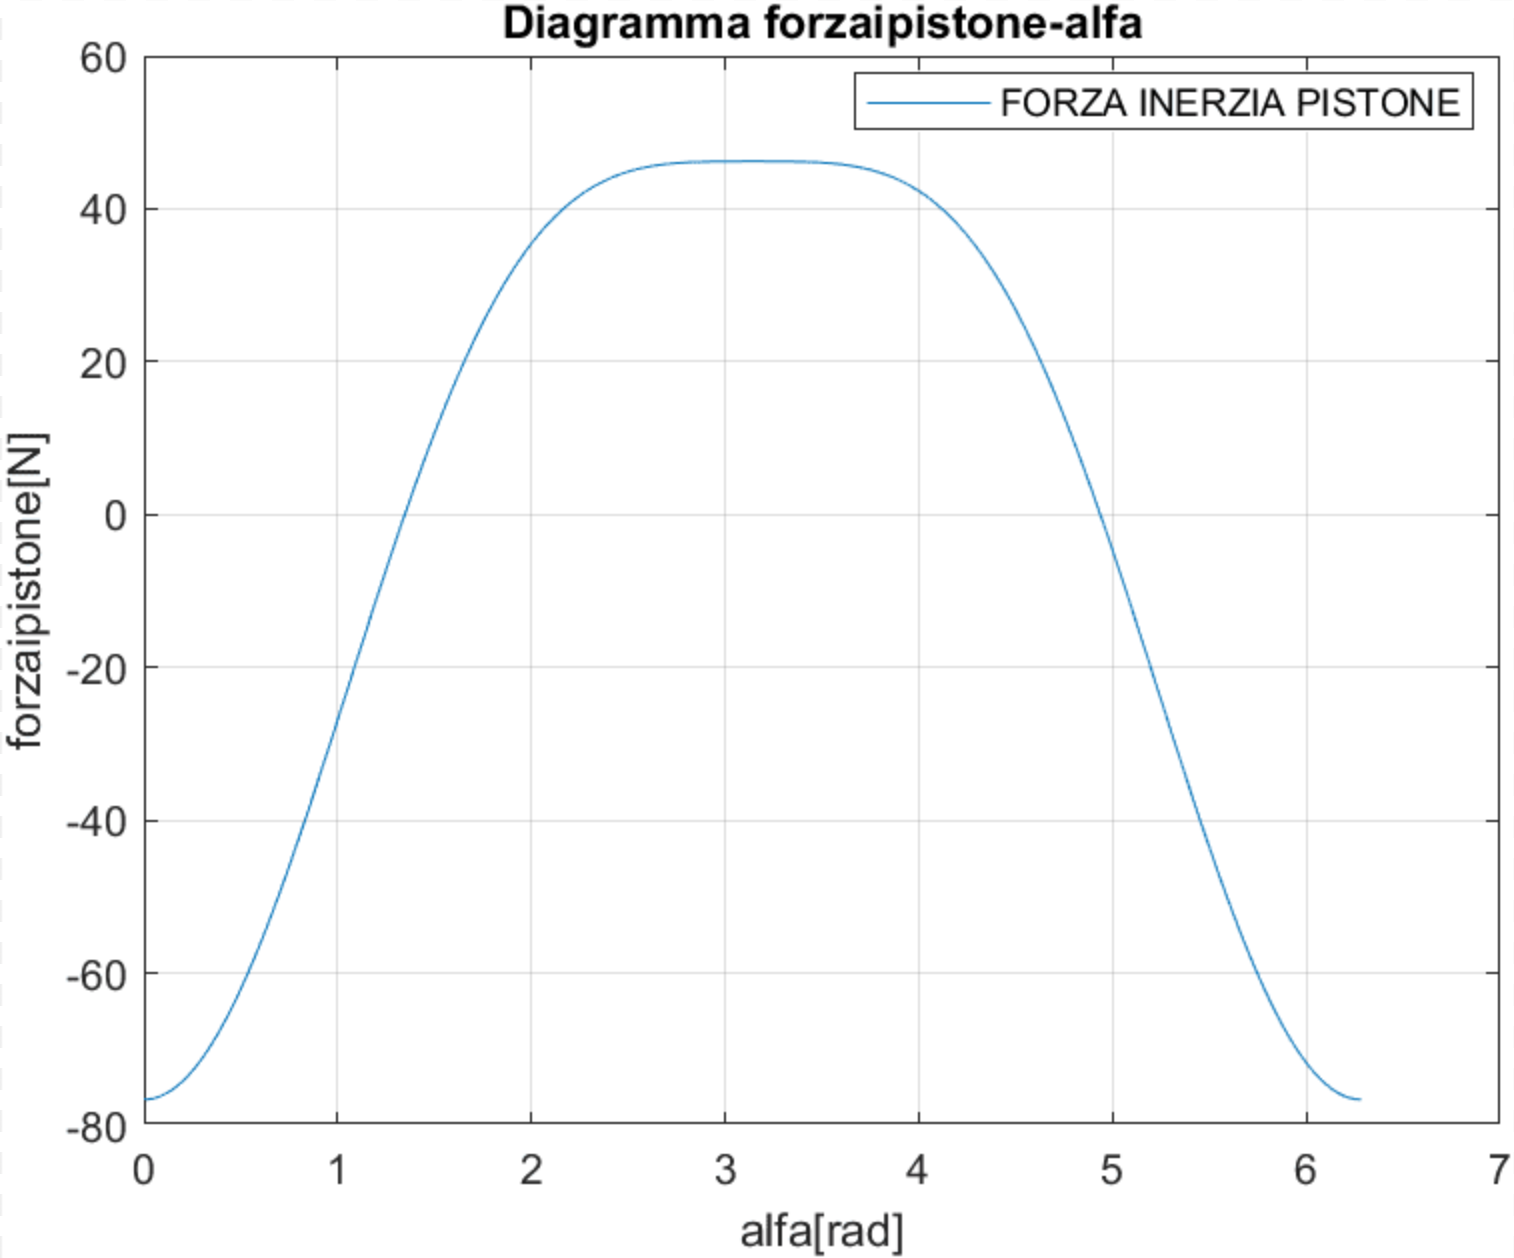
\includegraphics[scale=0.33]{Immagini/GraficoInerziaPistone.png}
    \caption{Forza dovuta all'inerzia del pistone al variare di $\alpha$}
    \label{fig:GraficoInerziaPistone}
\end{figure}
\begin{lstlisting}[frame=trBL]
%Grafico forza inerzia al variare di alfa

mp=0.11238 %massa pistone [Kg]
forzaipistone=-mp*accelerazione;
plot(alfa,forzaipistone);

xlabel('alfa[rad]'),ylabel('forzaipistone[N]'),
      title('Diagramma forzaipistone-alfa'),
      grid on;xlim(0,2*pi);
\end{lstlisting}
\paragraph{Forza dovuta all'inerzia della biella} Per studiare le sollecitazioni agenti sul pistone dovute alla biella è necessario fare una semplificazione. Si passa dallo studio di un corpo rigido tridimensionale avente massa e tensore di inerzia fissati, all’analisi di un sistema equivalente costituito da due masse puntiformi concentrate alle estremità.\\
Per poter adoperare questo stratagemma, bisogna imporre che l’energia cinetica rimanga invariata, così come il baricentro.\\
Condizioni per le quali le precedenti assunzioni sono verificate: 
\begin{equation}
    m_A+m_B=m
\end{equation}
\begin{equation}
    m_Aa^2+m_Bb^2+J_0=J
\end{equation}
\begin{equation}
    m_Aa=m_Bb
\end{equation}
\begin{figure}[h]
\centering
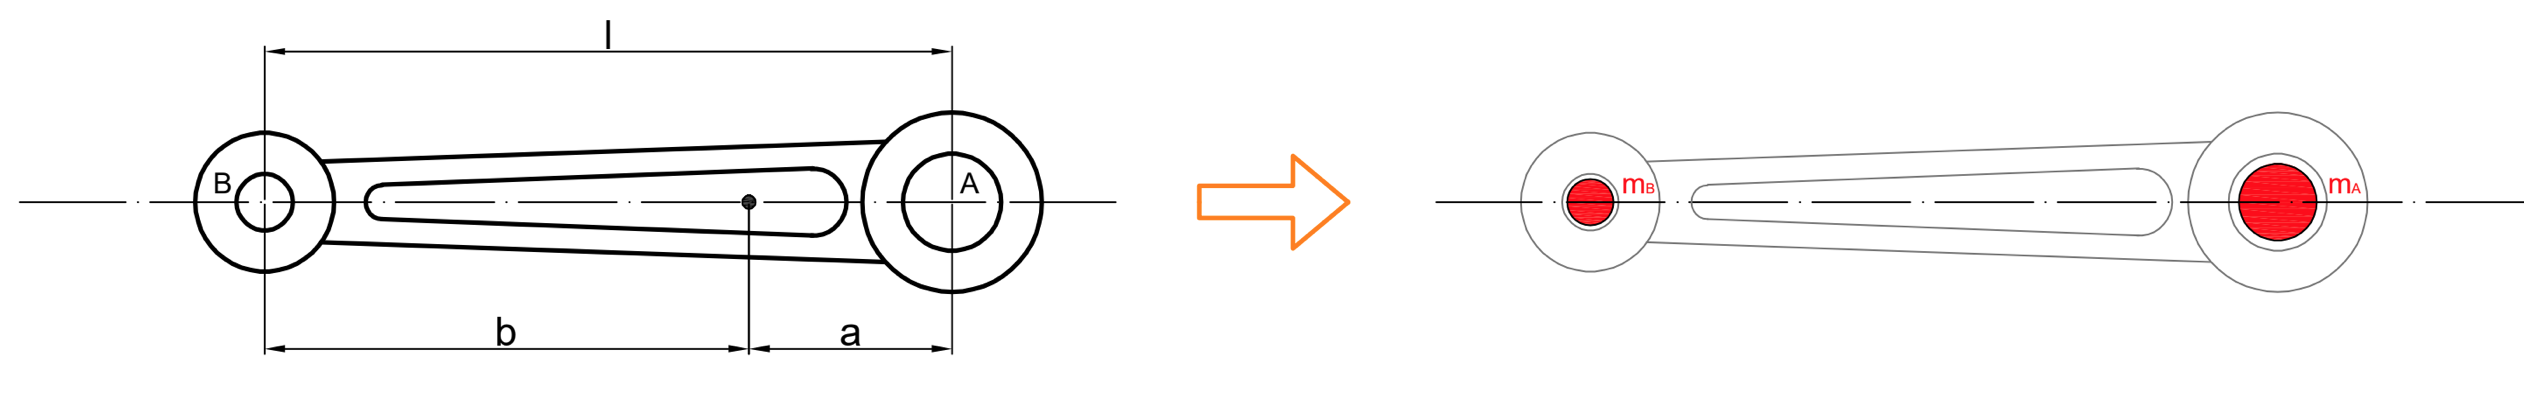
\includegraphics[scale=0.3]{Immagini/SostituzioneBiella.png}
\caption{Semplificazione per lo studio della biella}
\label{fig:SostituzioneBiella}
\end{figure}
\\
I termini $m_A$ e $m_B$ sono le due masse, $J_0$ è il momento d'inerzia puro, m è la massa della biella e $J$ è il suo momento di inerzia rispetto a un asse baricentrico ortogonale al piano del moto. \\
Il termine $J_0$ è un termine fittizio che è necessario introdurre come artificio algebrico (talvolta trascurabile) per steli snelli e che quasi sempre corrisponde ad una correzione di segno negativo. \\
Le distanze a e b sono prese in valore assoluto dal baricentro G ai punti A e B nei quali sono collocate $m_A$ e $m_B$.\\
Dalle condizioni scritte precedentemente si ottiene: 
\begin{equation}
    m_A=\frac{mb}{l}
\end{equation}
\begin{equation}
    m_B=\frac{ma}{l}
\end{equation}
\begin{equation}
    J_0=J-mab
\end{equation}
Dall’analisi delle proprietà di massa della biella su SOLIDWORKS (Fig.\ref{fig:CaratteristicheBiella}) è stato possibile ricavare la posizione del baricentro, quindi le distanze a e b e il momento d’inerzia J. 
\begin{equation}
    J\left(P_z\right)=6,5311{\cdot10}^{-5}\ kgm^2
\end{equation}
\begin{equation}
    a=33.16{\cdot10}^{-3}\ m
\end{equation}
\begin{equation}
    b=l-a=\left(85-33,16\right){\cdot10}^{-3}m=51,84{\cdot10}^{-3}\ m.
\end{equation}
Noti questi parametri, si ricavano dalle formule prima citate le grandezze associate allo studio della biella: 
\begin{equation}
    m_B=0,0205\ kg
\end{equation}
\begin{equation}
    m_A=m-m_B=\left(52,61{\cdot10}^{-3}-0,0205\right)\ kg=0,03209\ kg
\end{equation}
\begin{equation}
    J_0=-2,5126{\cdot10}^{-5}\ kgm^2.
\end{equation}
Avendo supposto di avere parte della massa di biella concentrata sul piede, essa durante il moto sarà soggetta a un’accelerazione che si tradurrà in una forza d’inerzia trasmessa al pistone.\\
La forza d’inerzia sarà: 
\begin{equation}
    F_i=-m_B\cdot a_{\mbox{pistone}}
\end{equation}
il cui andamento è stato ricavato mediante uno script Matlab.
\begin{figure}[h]
    \centering
    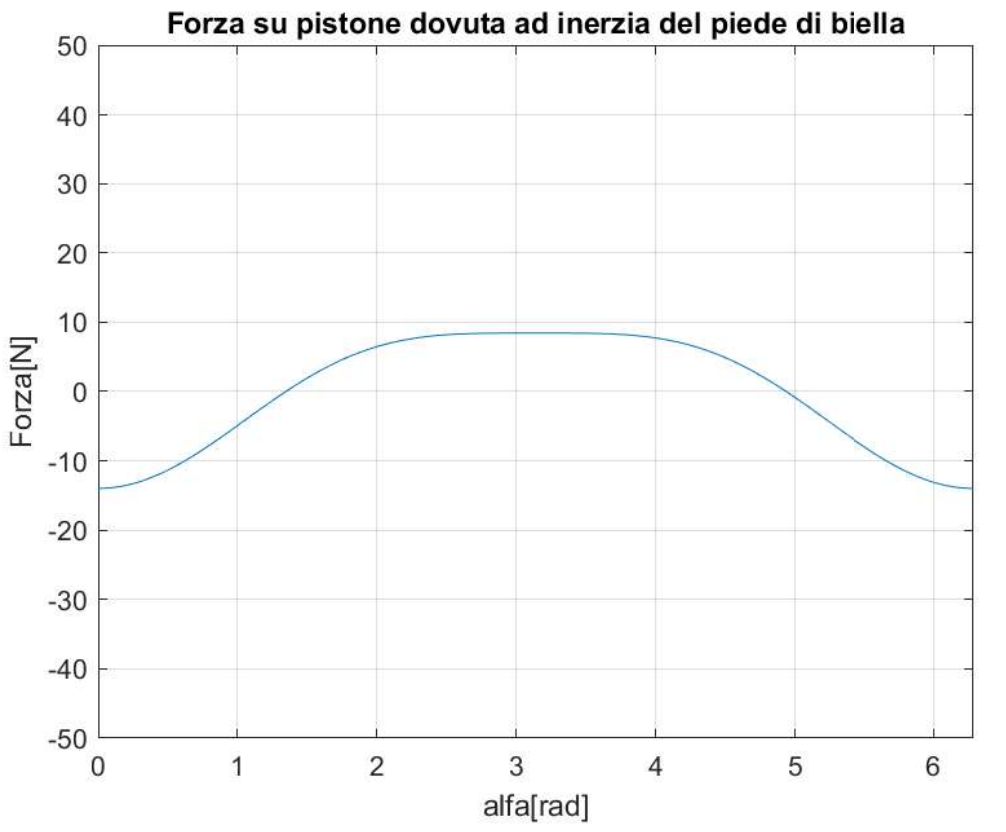
\includegraphics[scale=0.6]{Immagini/GraficoInerziaPiede.png}
    \caption{Andamento della forza di inerzia dovuta al piede di biella}
    \label{fig:GraficoInerziaPiede}
\end{figure}
\begin{lstlisting}[frame=trBL]
%Grafico forze di inerzia dovute alla massa del piede di biella

mbiella=52.61*(10^-3); %[kg]
b=33.16*(10^-3); %distanza tra centro di massa e testa di biella [m]
a=51.84*(10^-3); %distanza tra centro di massa e piede di biella[m]
l=85*(10^-3); %interasse tra testa e piede di biella [m]
mB=(mbiella*b)*(l^-1);
Forzapistone3=-mB*accelerazione;
plot(alfa,Forzapistone3);
xlabel('alfa[rad]'),ylabel('Forza[N]'),
      title('Forza su pistone dovuta ad inerzia de piede di biella'),
      grid on,xlim([0 2*pi]),ylim([-50 50]);
\end{lstlisting}
\paragraph{Forza dovuta all'inerzia dello spinotto} Essendo lo spinotto solidale al pistone durante il moto, anch’esso contribuirà a geneare una componente d’inerzia sul pistone. \\
Tale forza può essere quantificata come: 
\begin{equation}
    F_i=-m_{\mbox{spinotto}}\cdot a_{\mbox{pistone}}
\end{equation}
il cui andamento è ricavato mediante uno script Matlab.
\newpage
\begin{figure}[h]
    \centering
    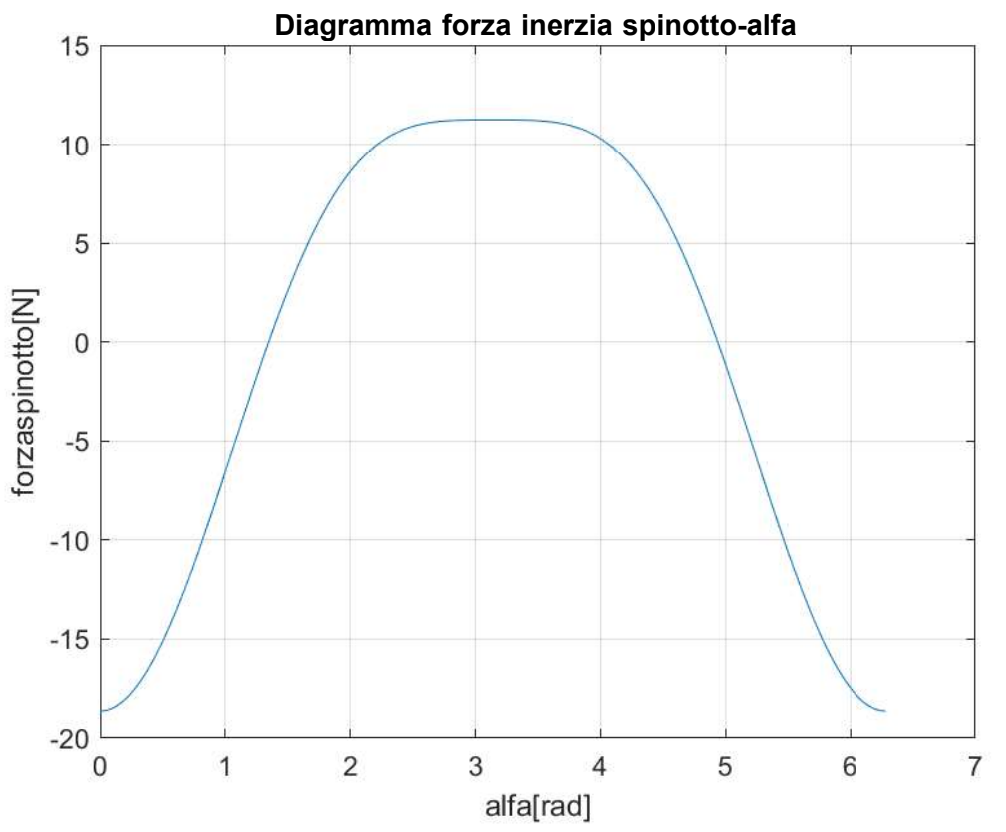
\includegraphics[scale=0.5]{Immagini/GraficoInerziaSpinotto.png}
    \caption{Andamento della forza di inerzia dovuta allo spinotto}
    \label{fig:GraficoInerziaSpinotto}
\end{figure}

\begin{lstlisting}[frame=trBL]
%Grafico forze di inerzia dovute alla massa dello spinotto

mspinotto=27.36*(10^-3); %[kg]
forzaspinotto=-mspinotto*accelerazione;
plot(alfa,forzaspinotto);
xlabel('alfa[rad]'),ylabel('forzaspinotto[N]'),
       title('Diagramma forza inerziaspinotto-alfa'),
       grid on;xlim(0,2*pi);
\end{lstlisting}
Di seguito si riportano in un unico grafico tutti i contributi di forze dovuti alla pressione e alle inerzie che agiscono sul pistone.\\
Si può notare come queste ultime siano trascurabili rispetto all’entità della forza generata dalla pressione del fluido.
\begin{figure}[h]
\centering
   {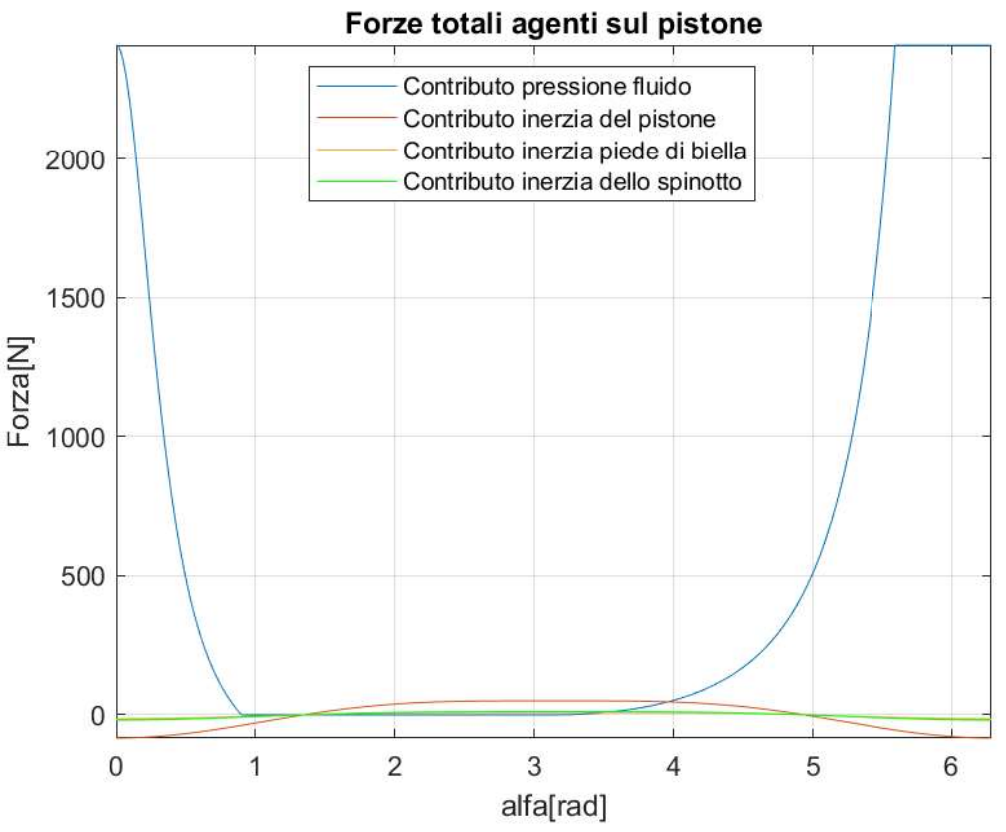
\includegraphics[width=.48\textwidth]{Immagini/GraficoInsiemeForze1.png}} \quad
   {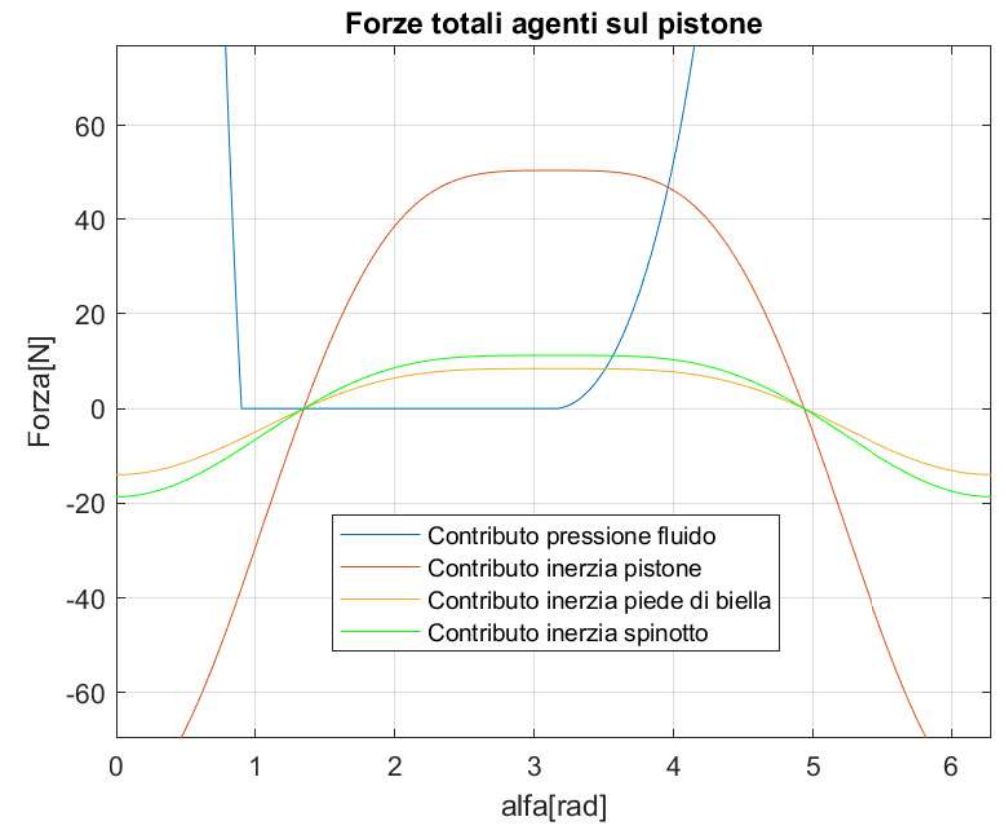
\includegraphics[width=.48\textwidth]{Immagini/GraficoInsiemeForze2.png}}
\caption{Insieme delle forze agenti sul pistone al variare di $\alpha$}
\label{fig:GraficoInsiemeForze}
\end{figure}
\newpage
\begin{lstlisting}[frame=trBL]
%Grafico insieme delle forze

plot(alfatot,Forzapistone1);
hold on     
plot(alfa,forzaipistone);
plot(alfa,Forzapistone3);
plot(alfa,forzaspinotto,'g');
xlabel('alfa[rad]'),ylabel('Forza[N]'),
       title('Forze totali agenti sul pistone'),
       grid on,xlim([0 2*pi]),ylim([-50 50]);
hold off
\end{lstlisting}
Sommando tutti i contributi delle forze agenti sul pistone la risultante avrà un andamento come mostrato in figura:
\begin{figure}[h]
    \centering
    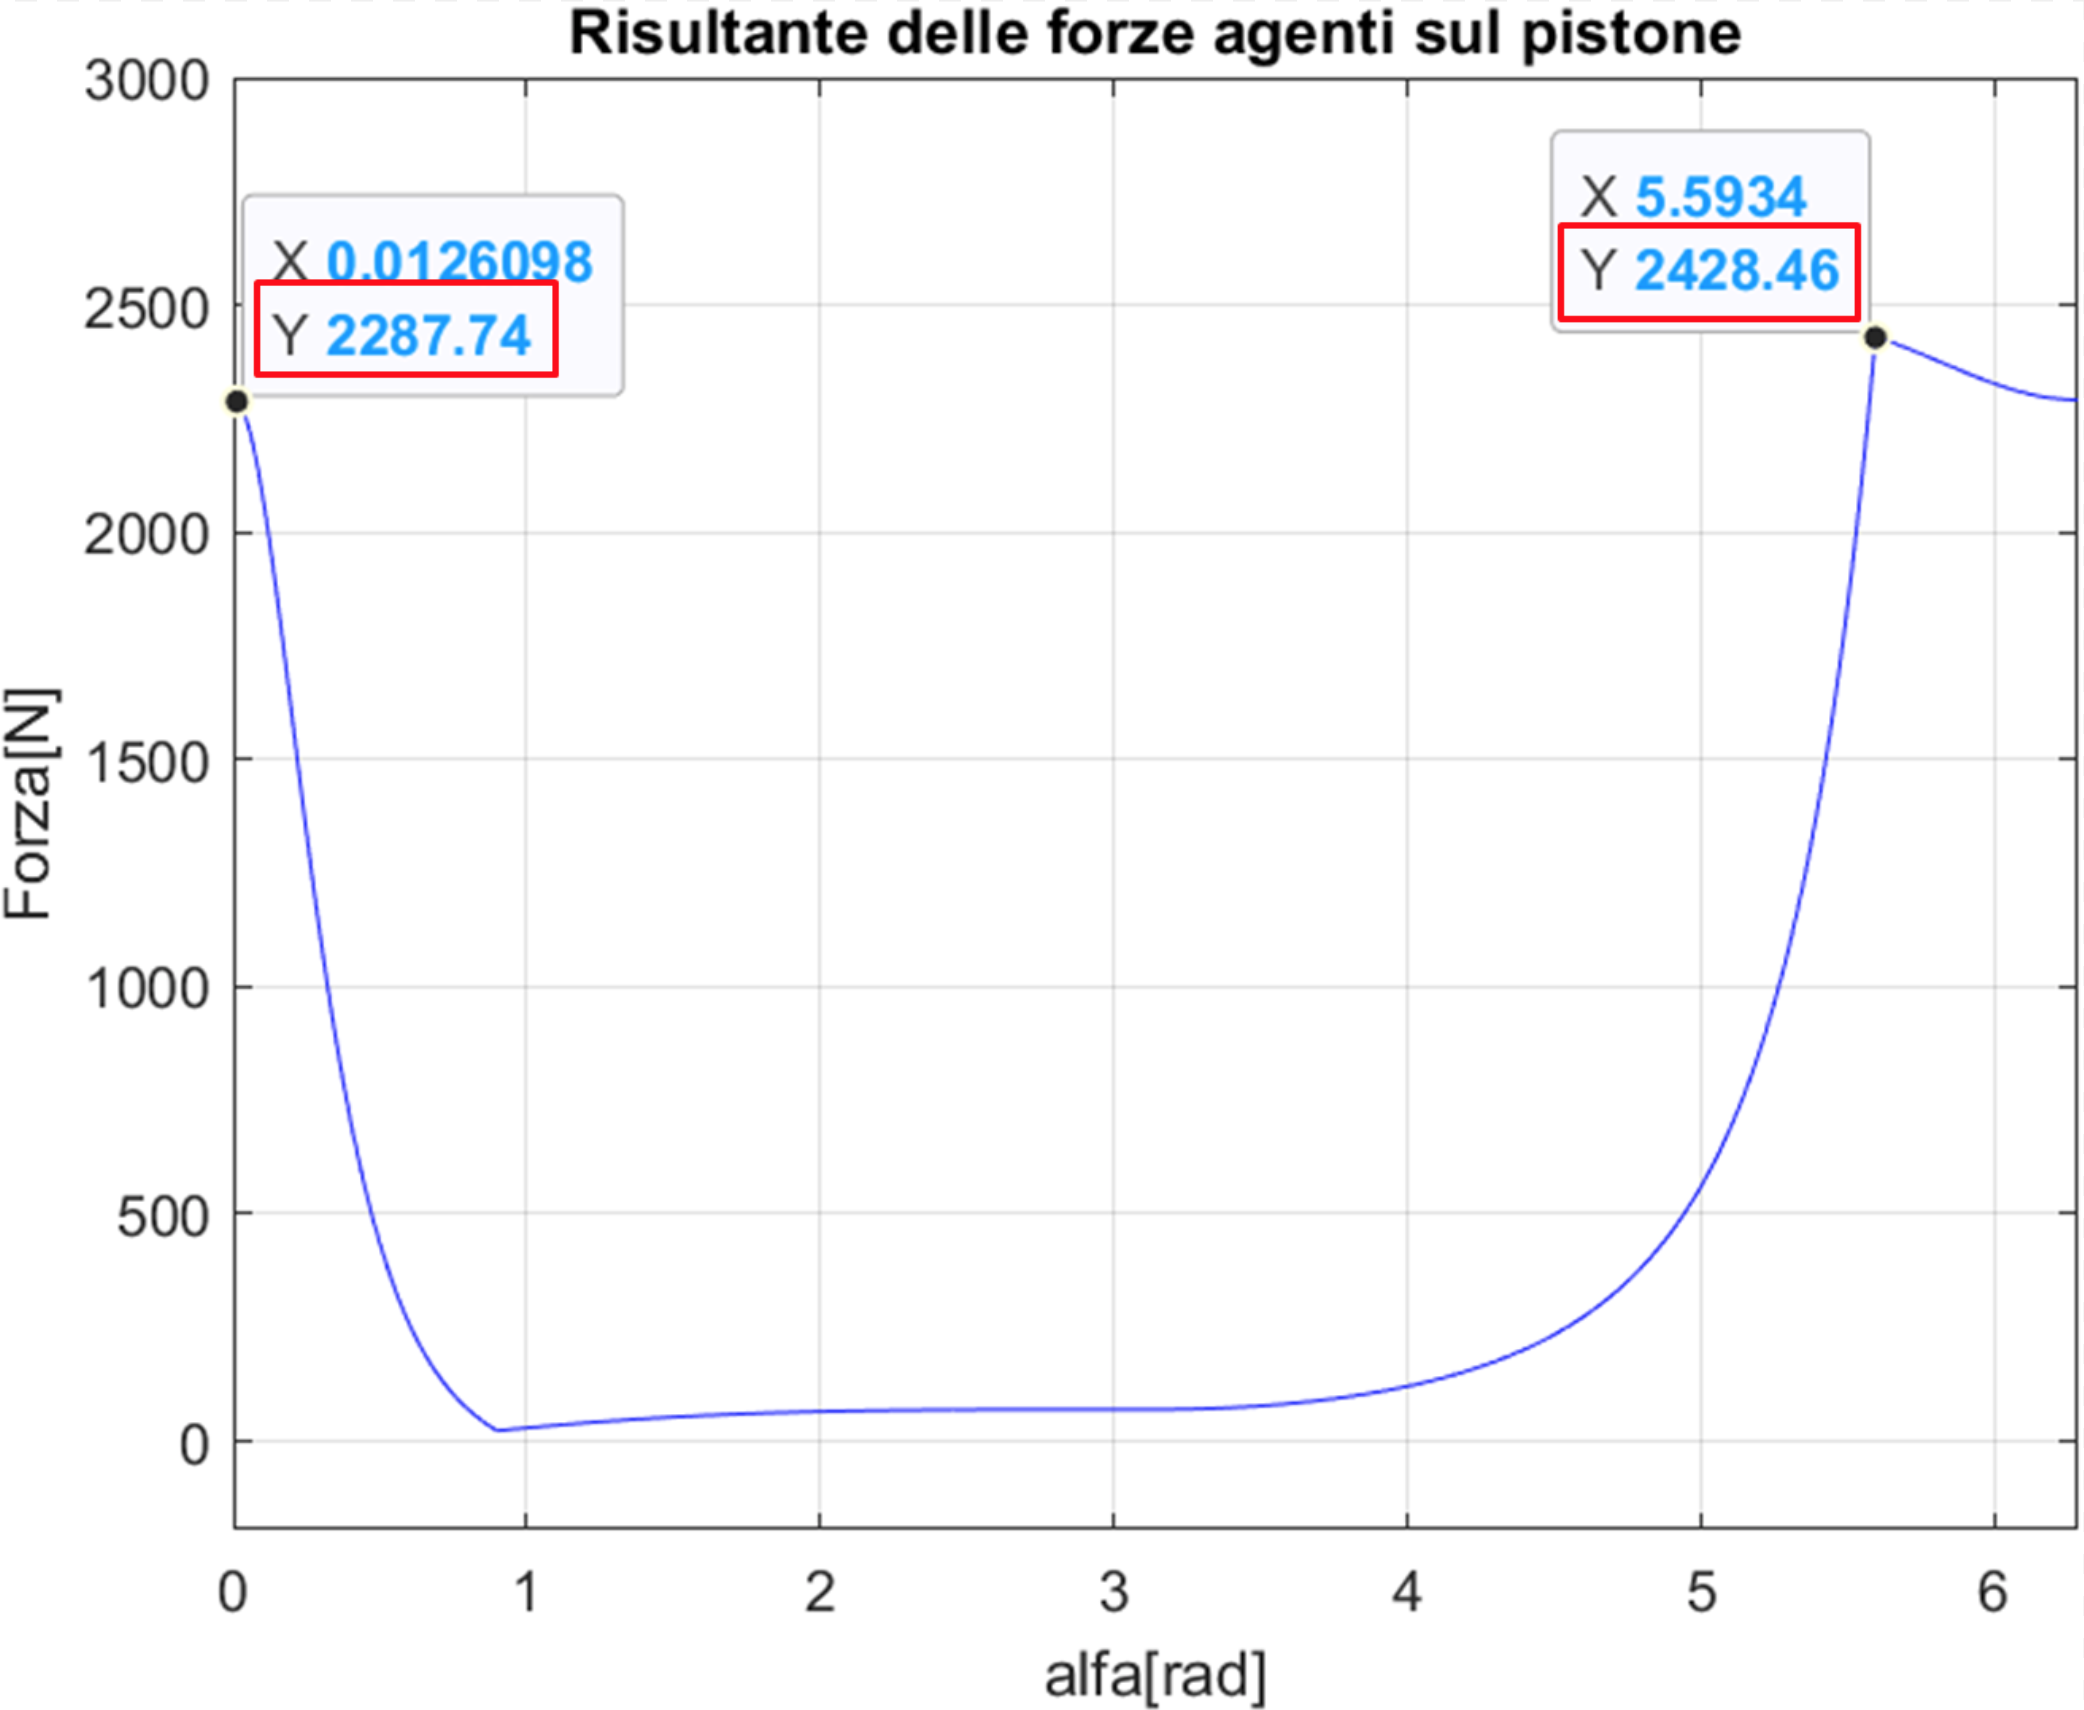
\includegraphics[scale=0.3]{Immagini/GraficoForzaRisultante.png}
    \caption{Andamento della forza risultante sul pistone al variare di $\alpha$}
    \label{fig:GraficoForzaRisultante}
\end{figure}
\begin{lstlisting}[frame=trBL]
%Grafico andamento forza totale

Ftot=forzaspinotto+Forzapistone3,+Forzapistone1+forzaipistone;
plot(alfa,Ftot)

xlabel('alfa[rad]'),ylabel('Forza[N]'),
      title('Risultante delle forze agenti sulpistone'),
      grid on,xlim([0 2*pi]),ylim([-100 3000]);
\end{lstlisting}
Come è possibile dedurre dal grafico, le posizioni in cui il pistone è soggetto a maggiori sollecitazioni comprendono dal punto di fine compressione a quello di inizio espansione.\\
La forza massima agente si può assumere da grafico pari a 2428.46 N.\\
Per i calcoli strutturali che verranno effettuati successivamente si ipotizzerà di avere una forza massima agente sul pistone pari a $F_{\mbox{pistone}} = 2500\ N$, contemplando già da qui un fattore di sicurezza per considerare eventuali valutazioni approssimative effettuate durante l’analisi dei carichi del cinematismo (per esempio la considerazione del ciclo ideale per i calcoli, il fatto che la modellazione CAD non è perfettamente fedele alla realtà e la scelta del materiale). 
\subsubsection{Spinotto}
Le forze che agiscono sullo spinotto sono le stesse che agiscono sul pistone e quindi quelle che possono essere osservate in Fig.\ref{fig:GraficoForzaRisultante}.\\
Quindi anche in questo caso per i calcoli strutturali, esattamente come quanto detto per il pistone, considereremo una forza massima agente pari a $F_{\mbox{spinotto}} = 2500\ N$. 
\subsubsection{Biella}
Le forze che agiscono sulla biella sono:
\paragraph{Forza agente sul piede di biella}La forza totale agente sul piede di biella è quella trovata precedentemente dovuta a pressione del fluido, inerzie di pistone, spinotto e piede di biella. \\
L’andamento in funzione dell’angolo di manovella è quindi analogo a quello osservato per il pistone (Fig.\ref{fig:GraficoForzaRisultante}).  La sollecitazione sulla biella si divide in due componenti, una parallela all’asse della biella (compressione) e una ortogonale (flessione). 
\paragraph{Forza di inerzia centrifuga sulla testa di biella}La forza di inerzia dovuta alla rotazione della testa di biella attorno all’asse dell’albero ha direzione radiale ed è indipendente, in modulo, dall’angolo di manovella $\alpha$.\\
Il modulo può essere quantificato con la seguente formula: 
\begin{equation}
    F_{c1}=m_Ar\omega^2
\end{equation}
con $m_A$ massa della testa di biella pari a 0,03209 kg, r raggio di manovella pari a 0,021 m e $\omega$ velocità angolare di rotazione pari a $\omega=\frac{2\pi n}{60}=161,27\ rad/s$.\\
Si ottiene quindi $F_{c1}=17,53\ N$.\\
\\
Bisogna tenere conto, inoltre, della forza rotante centrifuga dovuta al moto della manovella, secondo la formula 
\begin{equation}
    F_{c2}=m_mr_m\omega^2
\end{equation}
si ottiene quindi $F_{c2}=327,7\ N$.\\
\\
In conclusione, la forza risultante agente sulla testa di  biella corrisponde a:
\begin{equation}
    F_c=F_{c1}+F_{c2}=\left(17,53+327,7\right)\ N=345,2\ N
\end{equation}
\newpage
\begin{figure}[h]
    \centering
    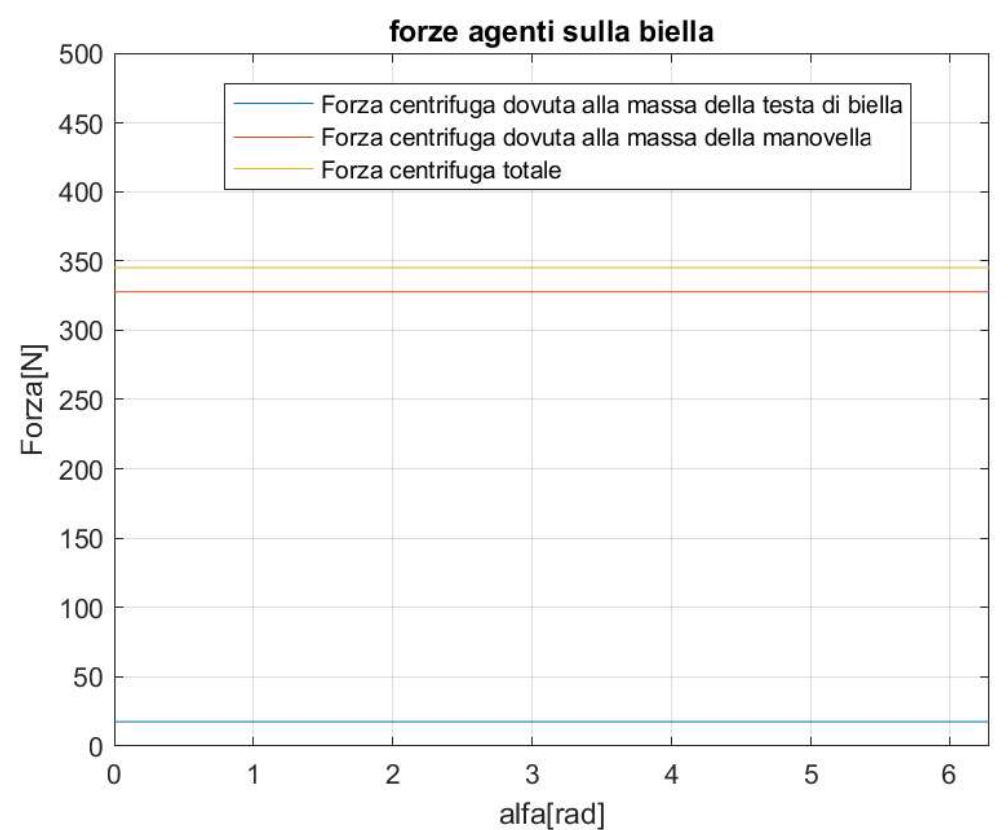
\includegraphics[scale=0.5]{Immagini/GraficoForzeCentrifugheBiella.png}
    \caption{Andamento forze centrifughe agenti sulla biella}
    \label{fig:GraficoForzeCentrifugheBiella}
\end{figure}
\begin{lstlisting}[frame=trBL]
%Calcolo forze su biella

%Dati
mB=0.03209; %massa B sistema equivalente biella [kg]
massaman=0.6; %massa di meta albero, ovvero della manovella [kg]
r=0.021; %raggio dimanovella [m]
n=1540; %velocita rotazione [giri/s]
l=0.085;
lambda=l*(r^-1); %[kg m^2]
Jo=-2.5126*(10^-5);

%Grandezze derivate
w=(2*pi*n)*(60^-1); %velocita angolare [rad/s]

%Forza centrifuga testa di biella
Fcent1=(mB)*r*w^2;
F=linspace(Fcent1,Fcent1,2000);
alfa=linspace(0,2*pi,2000);
plot(alfa, F);
xlabel('alfa[rad]'),ylabel('Forza[N]'),
      title('forze agenti sulla biella'),grid on,xlim([0 2*pi]);
      ylim([0 500]);
hold on
Fcent2=(massaman)*r*w^2;
F=linspace(Fcent2,Fcent2,2000);
alfa=linspace(0,2*pi,2000);
plot(alfa, F);
hold on
Ftot=Fcent1+Fcent2;
F=linspace(Ftot,Ftot,2000);
alfa=linspace(0,2*pi,2000);
plot(alfa, F);
hold off
\end{lstlisting}
\paragraph{Coppia di biella}
Ricordando la semplificazione ad uno schema equivalente adottato nello studio della biella è possibile stimare la coppia di inerzia rotante agente sul corpo.\\
La coppia di inerzia vale $-J_0\lambda\Omega^2\sin\alpha$.\\
Essa si può pensare come due forze di uguale intensità e direzione, ma di versi opposti, con la retta d’azione passante per A e per B e dirette perpendicolarmente all’asse di moto del pistone 
\begin{equation}
    F_{ci}=\left|\frac{J_0r}{l^2}\Omega^2sin{\left(\alpha\right)}\right|.
    \label{ForzaCoppiaBiella}
\end{equation}
\begin{figure}[h]
\centering
   {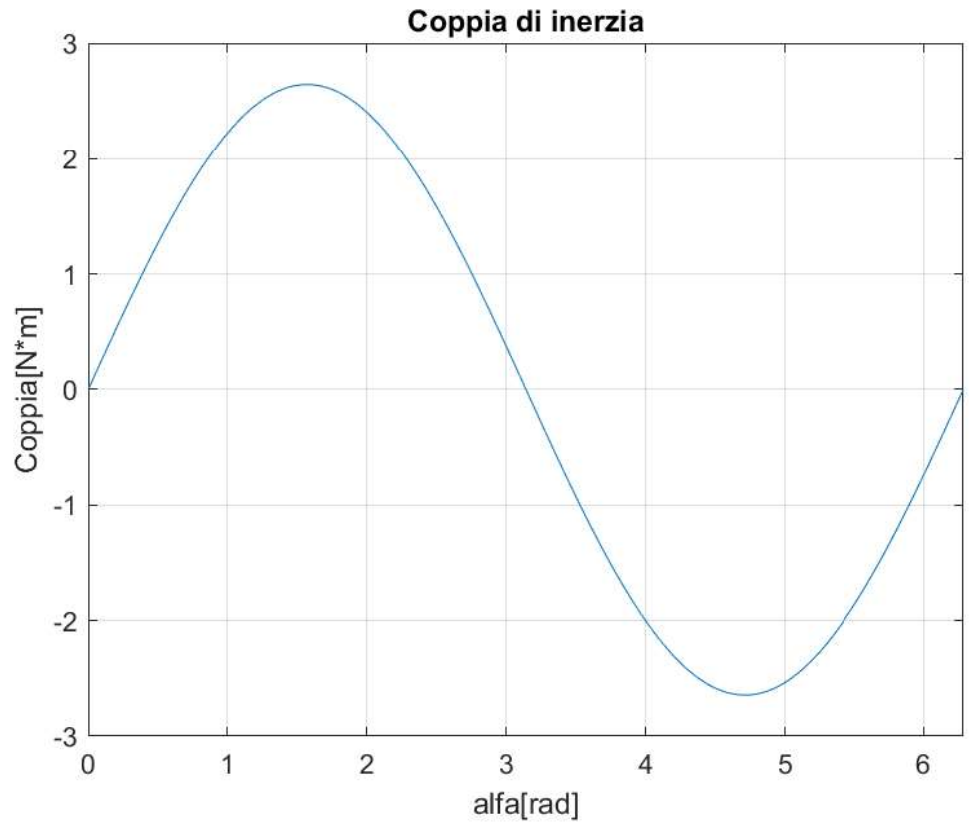
\includegraphics[width=.48\textwidth]{Immagini/GraficoCoppiaInerzia.png}} \quad
   {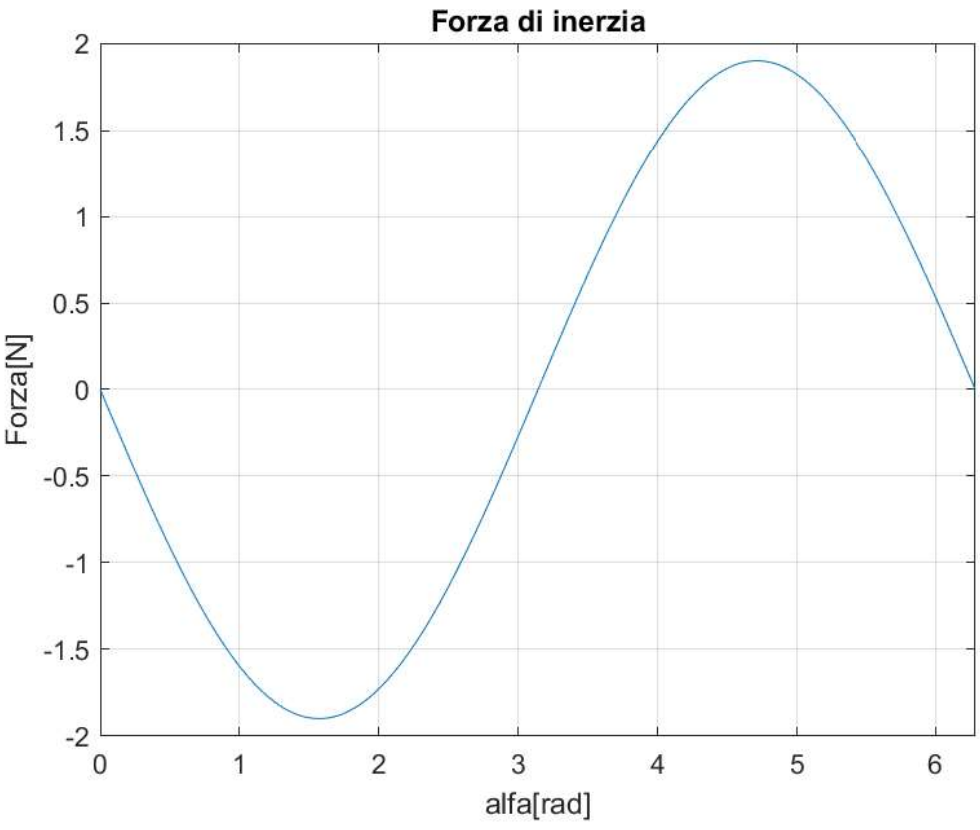
\includegraphics[width=.48\textwidth]{Immagini/GraficoForzaInerzia.png}}
\caption{Andamento della coppia e forza di inerzia al variare di $\alpha$}
\label{fig:GraficoInerziaBiella}
\end{figure}
\begin{lstlisting}[frame=trBL]
%Grafico coppia di inerzia
alfa=linspace(0,2*pi,2000);
Coppiainerzia=-Jo*lambda*w^2*(sin(alfa))
plot(alfa,Coppiainerzia);
xlabel('alfa[rad]'),ylabel('Coppia[N*m]'),
      title('Coppia di inerzia'),grid on,xlim([0 2*pi]);

%Grafico forza di inerzia
Finerzia=Jo*(r/(l^2))*(w^2)*sin(alfa);
plot(alfa,Finerzia);
xlabel('alfa[rad]'),ylabel('Forza[N]'),
      title('Forza di inerzia'),grid on,xlim([0 2*pi]);
\end{lstlisting}
\newpage
\subsubsection{Albero a gomiti}
\paragraph{Forza di inerzia centrifughe}
Le forze di inerzia centrifughe attorno all’asse di rotazione dell’albero corrispondono alle stesse agenti sulla testa di biella, calcolate in precedenza.\\
Quindi $F_c=345,2\ N$.\\
Tuttavia in questo caso, essendoci due manovelle sfasate tra loro di 180°, si formerà una coppia di forze rotanti di medesimo modulo, verso opposto e con rette di applicazioni non appartenenti allo stesso piano ortogonale all’asse.\\
Per tale motivo l’albero sarà equilibrato alle forze alterne del I ordine (traslazione), ma non al momento, manifestando un fenomeno di beccheggio durante il funzionamento. 
\begin{figure}[h]
\centering
   {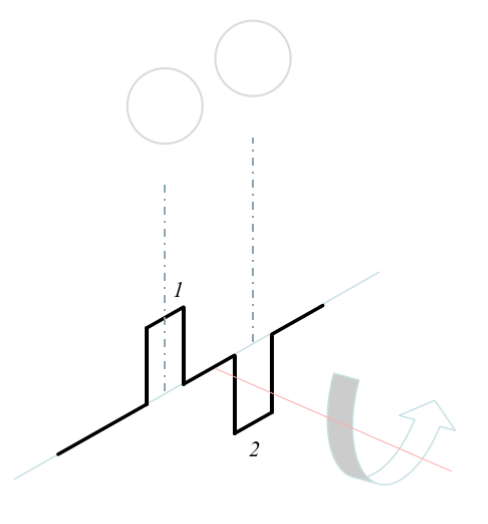
\includegraphics[width=.3\textwidth]{Immagini/Equilibratura1.png}} \quad
   {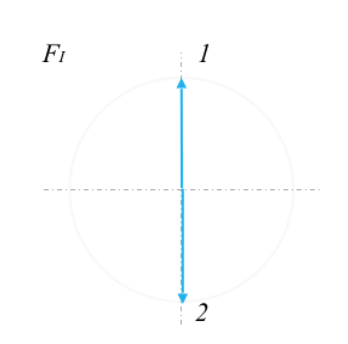
\includegraphics[width=.35\textwidth]{Immagini/Equilibratura2.png}}
\caption{Equilibratura albero a gomiti}
\label{fig:Equilibratura}
\end{figure}
\paragraph{Reazioni scaricate dalla biella sull'albero}Le forze che agiscono su pistone, spinotto e biella si scaricano sull’albero, secondo l’andamento trovato in precedenza (Fig.\ref{fig:GraficoForzaRisultante}).\\
Essendo doppi gli elementi del cinematismo di spinta, in totale sull’albero agiranno due azioni uguali, ma sfasate di 180° tra loro.\\
\begin{figure}[h]
    \centering
    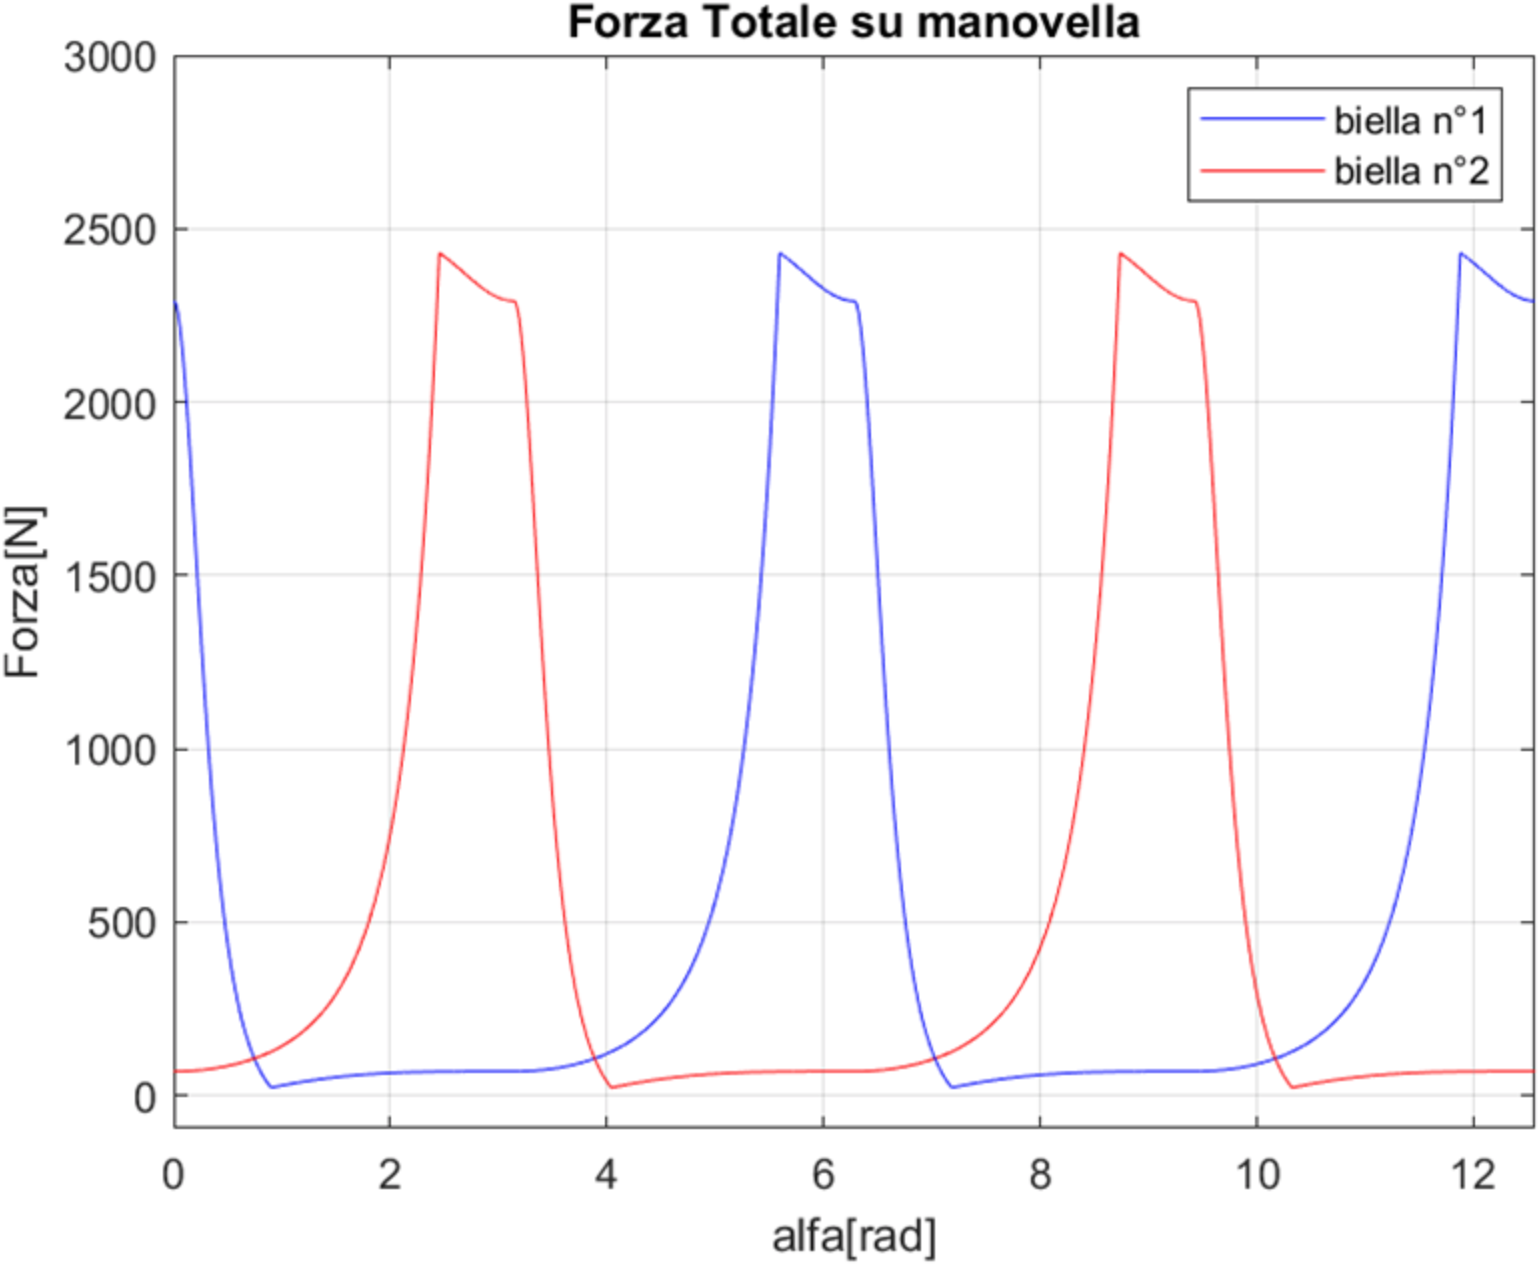
\includegraphics[scale=0.32]{Immagini/GraficoReazioniScaricateAlbero.png}
    \caption{Reazioni scaricate sull'albero al variare di $\alpha$}
    \label{fig:GraficoReazioniScaricateAlbero}
\end{figure}
\subsection{Andamento del momento torcente in funzione dell'angolo di manovella}
Per calcolare il momento torcente sarà necessario identificare la forza $F_{PB}$ ricavata a partire dalla forza totale, precedentemente ricavata, $F_{tot}$ agente sul pistone:
\begin{equation}
    F_{PB}=\frac{F_{tot}}{\cos\beta}
\end{equation}
\begin{figure}[h]
    \centering
    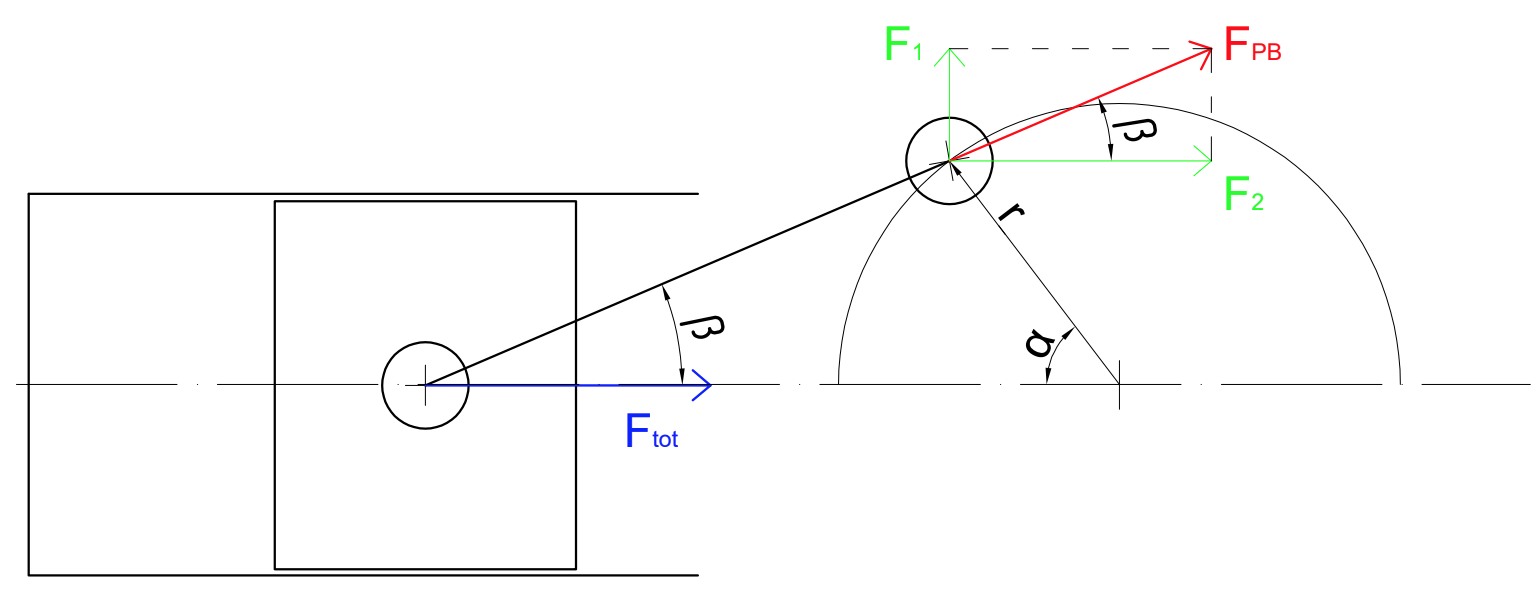
\includegraphics[scale=0.4]{Immagini/SchemaBiellaManovella.png}
    \caption{Schematizzazione delle forze di contributo al momento torcente}
    \label{fig:SchemaBiellaManovella}
\end{figure}
\\
Per quantificare il momento generato da tale forza attorno all’asse di rotazione sarà necessario scomporla in due componenti $F_1$ (ortogonale all’asse di moto del pistone) e $F_2$ (parallela all’asse di moto del pistone).
\begin{equation}
    F_2=F_{PB}\cos\beta
\end{equation}
\begin{equation}
    F_1=F_{PB}\sin\beta
\end{equation}
Ricavate queste componenti sarà quindi possibile calcolare i momenti, noti i rispettivi bracci d’azione.
\begin{equation}
    M_1=F_1r\cos\alpha
\end{equation}
\begin{figure}[h]
    \centering
    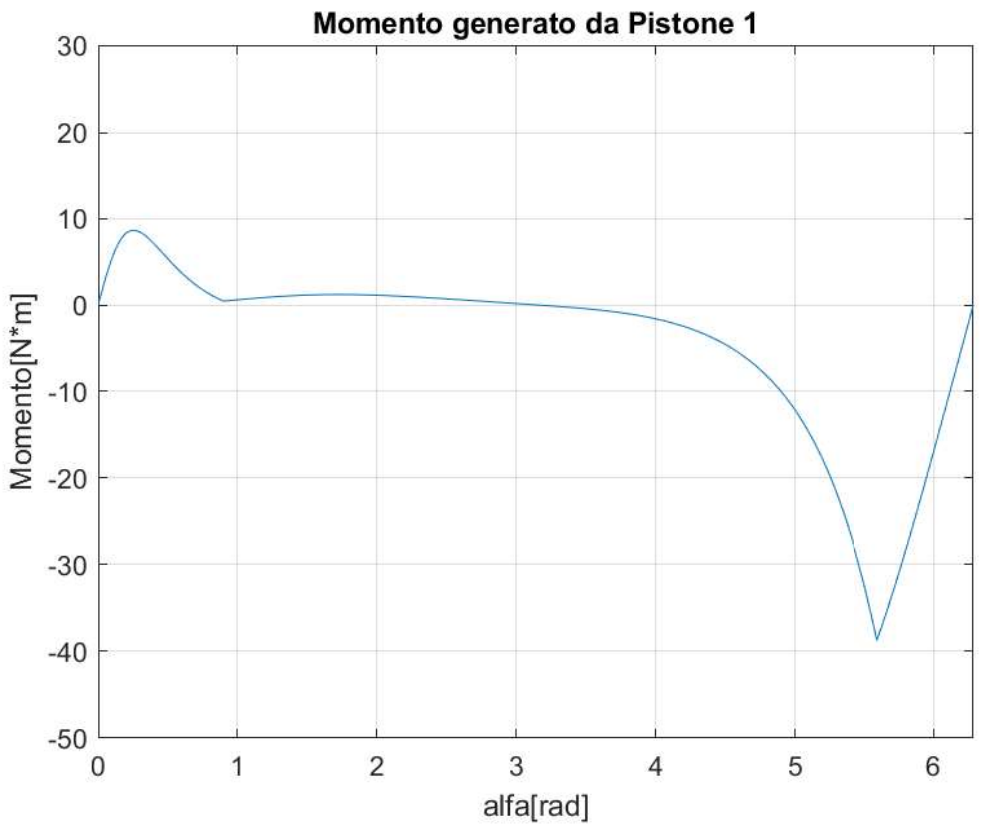
\includegraphics[scale=0.45]{Immagini/GraficoMomento1.png}
    \caption{Andamento del momento torcente generato dal primo cilindro}
    \label{fig:GraficoMomento1}
\end{figure}
\newpage
L’immagine di Fig.\ref{fig:GraficoMomento1} mostra l’andamento del momento torcente sull’albero a gomiti dovuto alle forze di pressione, all’inerzia del pistone, spinotto, testa e piede di biella. 
\begin{lstlisting}[frame=trBL]
%Grafico Momento torcente cilindro 1

senbeta=r/l*sin(alfatot);
cosbeta=sqrt(1-senbeta.^2);
Forzatrasmessa=Ftot./cosbeta;
F1=Forzatrasmessa.*senbeta;
F2=Forzatrasmessa.*cosbeta;
Mt1=r.*cos(alfatot).*F1+r.*sin(alfatot).*F2;
plot(alfatot,Mt1,'b');
xlabel('alfa[rad]'),ylabel('Momento[N*m]'),
      title('Momento generato da Pistone 1'),
      grid on,xlim([0 2*pi]),ylim([-50 50]);
\end{lstlisting}
L’andamento del momento torcente dovuto all’azione del secondo cilindro sarà uguale in modulo a quello ottenuto per il primo (Fig.\ref{fig:GraficoMomento1}), ma sfasato di 180°. 
\begin{equation}
    M_2=F_2r\sin\alpha
\end{equation}
\begin{figure}[h]
    \centering
    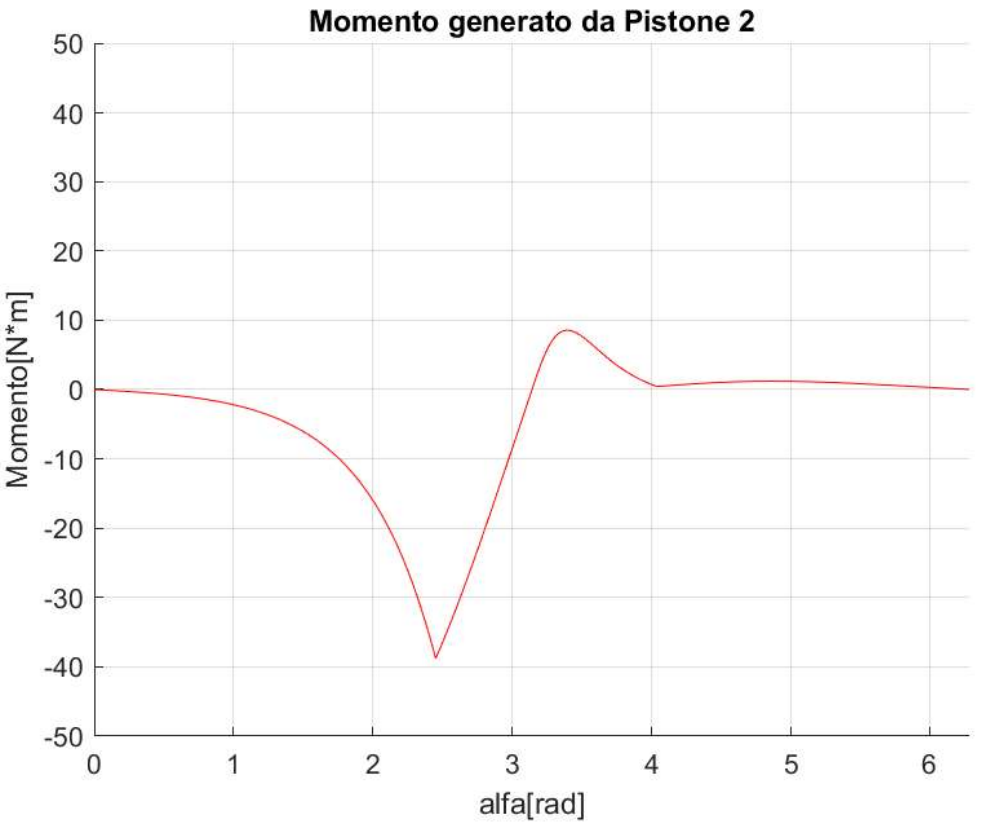
\includegraphics[scale=0.45]{Immagini/GraficoMomento2.png}
    \caption{Andamento del momento torcente generato dal secondo cilindro}
    \label{fig:GraficoMomento2}
\end{figure}
\begin{lstlisting}[frame=trBL]
%Momento torcente pistone 2

alfatot2=alfatot+3.14;
senbeta2=r/l*sin(alfatot2);
cosbeta2=sqrt(1-senbeta2.^2);
F12=Forzatrasmessa.*senbeta2;
F22=Forzatrasmessa.*cosbeta2;
Mt2=+r.*cos(alfatot2).*F12-r.*sin(alfatot2).*F22;
plot(alfatot2,Mt2,'r');
hold on
plot(alfatot2-2*pi,Mt2,'r');

xlabel('alfa[rad]'),ylabel('Momento[N*m]'),
      title('Momento generato da Pistone 2'),
      grid on,xlim([0 2*pi]),ylim([-50 50]);
\end{lstlisting}
In aggiunta bisognerebbe considerare anche il contributo in termini di momento dovuto alle forze derivanti dal momento di inerzia della biella J:
\begin{equation}
    M_{ci}=F_{ci}r\cos\alpha
\end{equation}
con $F_{ci}$ da eq.(\ref{ForzaCoppiaBiella}), il cui andamento era già stato riportato in Fig.\ref{fig:GraficoInerziaBiella}.
\begin{figure}[h]
    \centering
    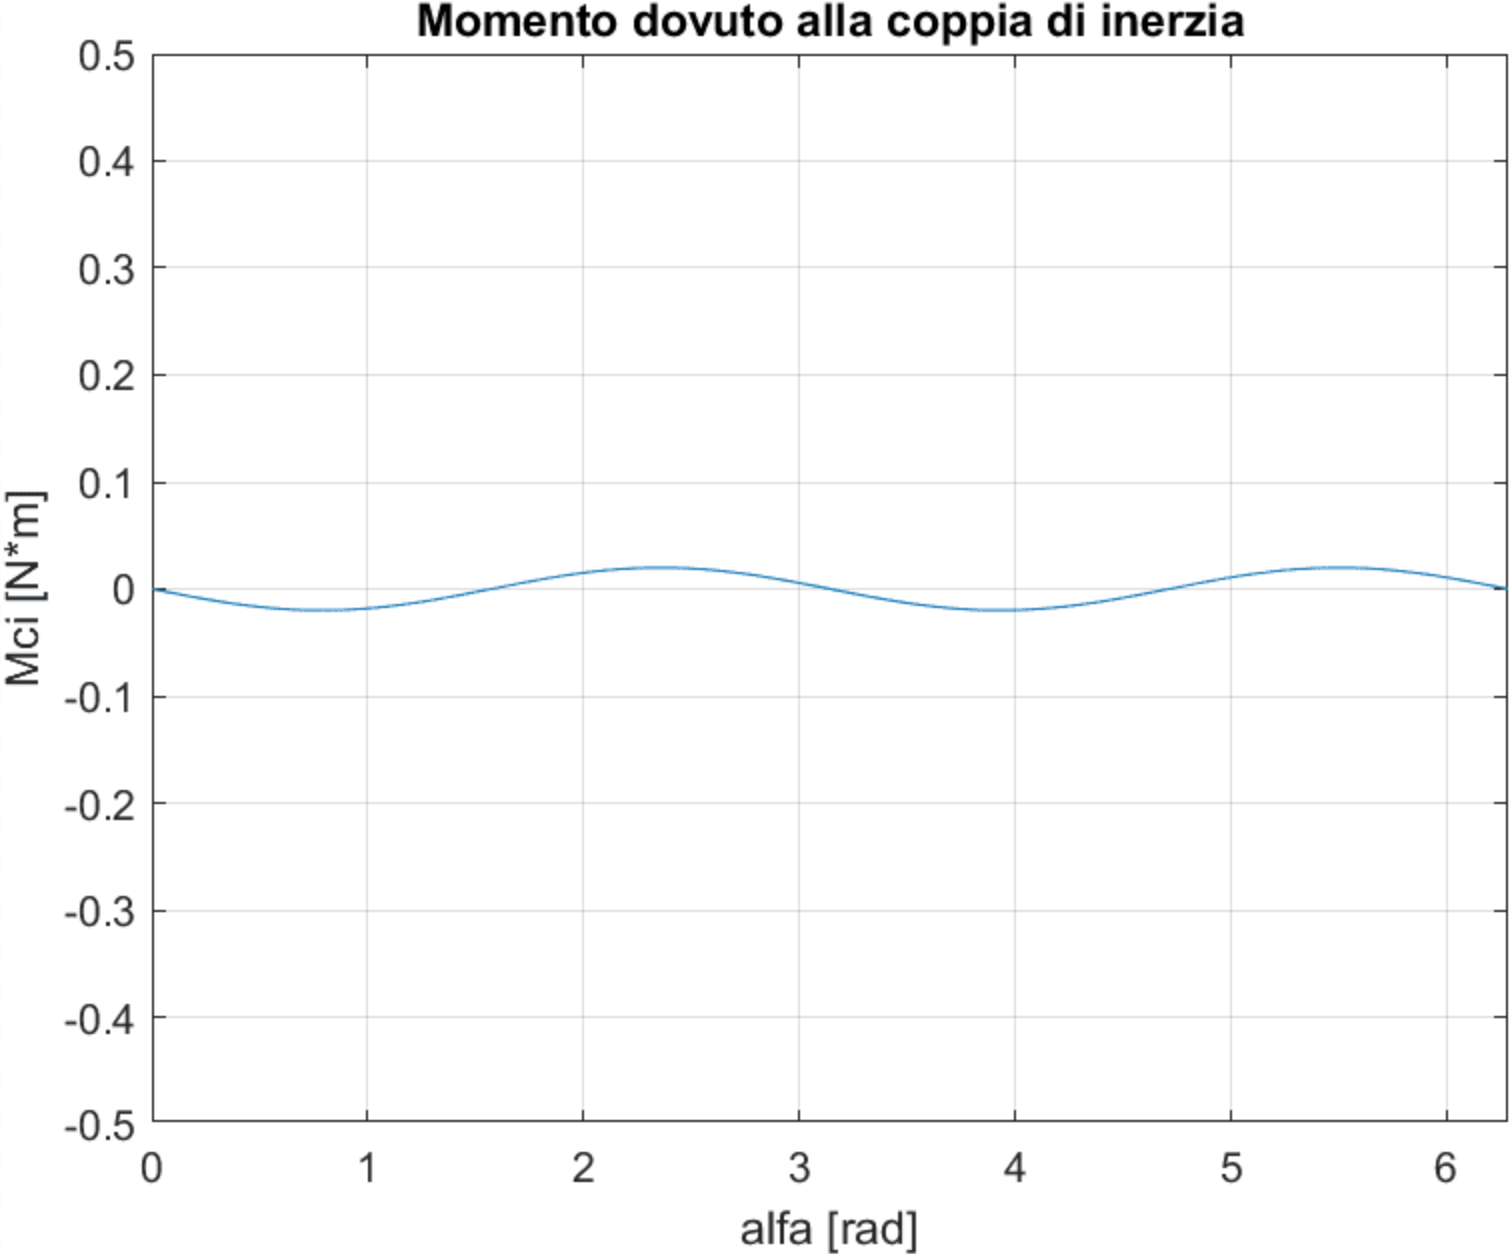
\includegraphics[scale=0.3]{Immagini/GraficoMomentoCoppiaBiella.png}
    \caption{Andamento del momento torcente dovuto alle forze di inerzia della biella}
    \label{fig:GraficoMomentoCoppiaBiella}
\end{figure}
\begin{lstlisting}[frame=trBL]
% Momento torcente dovuto alla coppia di inerzia della biella

Mci=Finerzia*r.*cos(alfa);
plot(alfa,Mci);
xlabel('alfa [rad]'),ylabel('Mci [N*m]'),
      title('Momento dovuto alla coppia di inerzia'),
      grid on, xlim([0 2*pi]),ylim([-0.5 0.5]);
\end{lstlisting}
Com’è possibile osservare dal grafico ottenuto in Matlab questo contributo risulta trascurabile in termini quantitativi rispetto ad $M_1$ ed $M_2$.\\
Quindi questo contributo non sarà tenuto in considerazione nemmeno per il momento torcente complessivamente generato sull'albero a gomiti. \\
In fase di calcolo si terrà comunque conto indirettamente di questo contributo, assumendo un minimo coefficiente di sicurezza, che contempli il fatto che il momento potrebbe essere leggermente superiore rispetto al valore considerato.\\
\\
Di seguito vengono riportati i due andamenti precedentemente ottenuti all’interno di un unico grafico.
\begin{figure}[h]
    \centering
    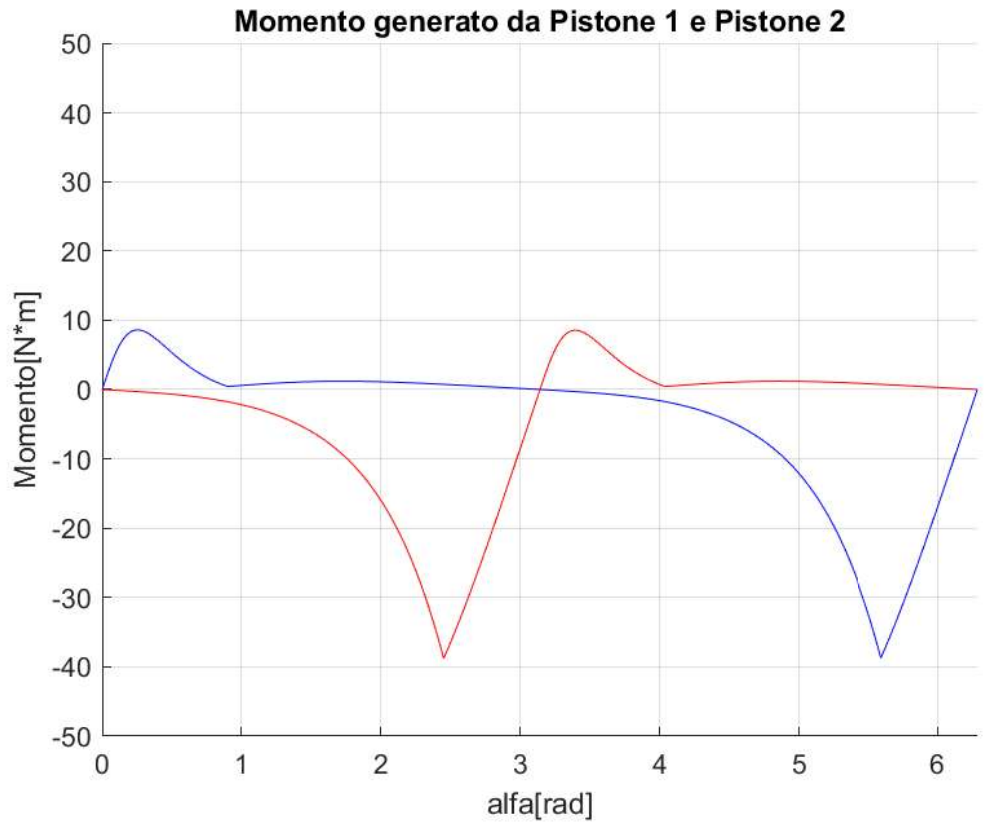
\includegraphics[scale=0.5]{Immagini/GraficoMomento1e2.png}
    \caption{Andamento dei due momenti generati all'interno di un unico giro di manovella}
    \label{fig:GraficoMomento1e2}
\end{figure}
\begin{lstlisting}[frame=trBL]
%%Momento torcente dei due pistoni insieme

%Momento torcente pistone 1
senbeta=r/l*sin(alfatot);
cosbeta=sqrt(1-senbeta.^2);
Forzatrasmessa=Forzaris./cosbeta;
F1=Forzatrasmessa.*senbeta;
F2=Forzatrasmessa.*cosbeta;
Mt1=r.*cos(alfatot).*F1+r.*sin(alfatot).*F2;
plot(alfatot,Mt1,'b');

hold on       %del momento torcente 1

%Momento torcente pistone 2
alfatot2=alfatot+3.14;
senbeta2=r/l*sin(alfatot2);
cosbeta2=sqrt(1-senbeta2.^2);
F12=Forzatrasmessa.*senbeta2;
F22=Forzatrasmessa.*cosbeta2;
Mt2=+r.*cos(alfatot2).*F12-r.*sin(alfatot2).*F22;
plot(alfatot2,Mt2,'r');
hold on       %del momento torcente 2
plot(alfatot2-2*pi,Mt2,'r');

xlabel('alfa[rad]'),ylabel('Momento[N*m]'),
      title('Momento generato da Pistone 1 e Pistone 2'),
      grid on,xlim([0 2*pi]),ylim([-50 50]);

hold off       %dei due momenti torcenti
\end{lstlisting}
Il momento torcente totale relativo ai due cilindri sarà definito come:
\begin{equation}
    M=M_1+M_2.
\end{equation}
\begin{figure}[h]
    \centering
    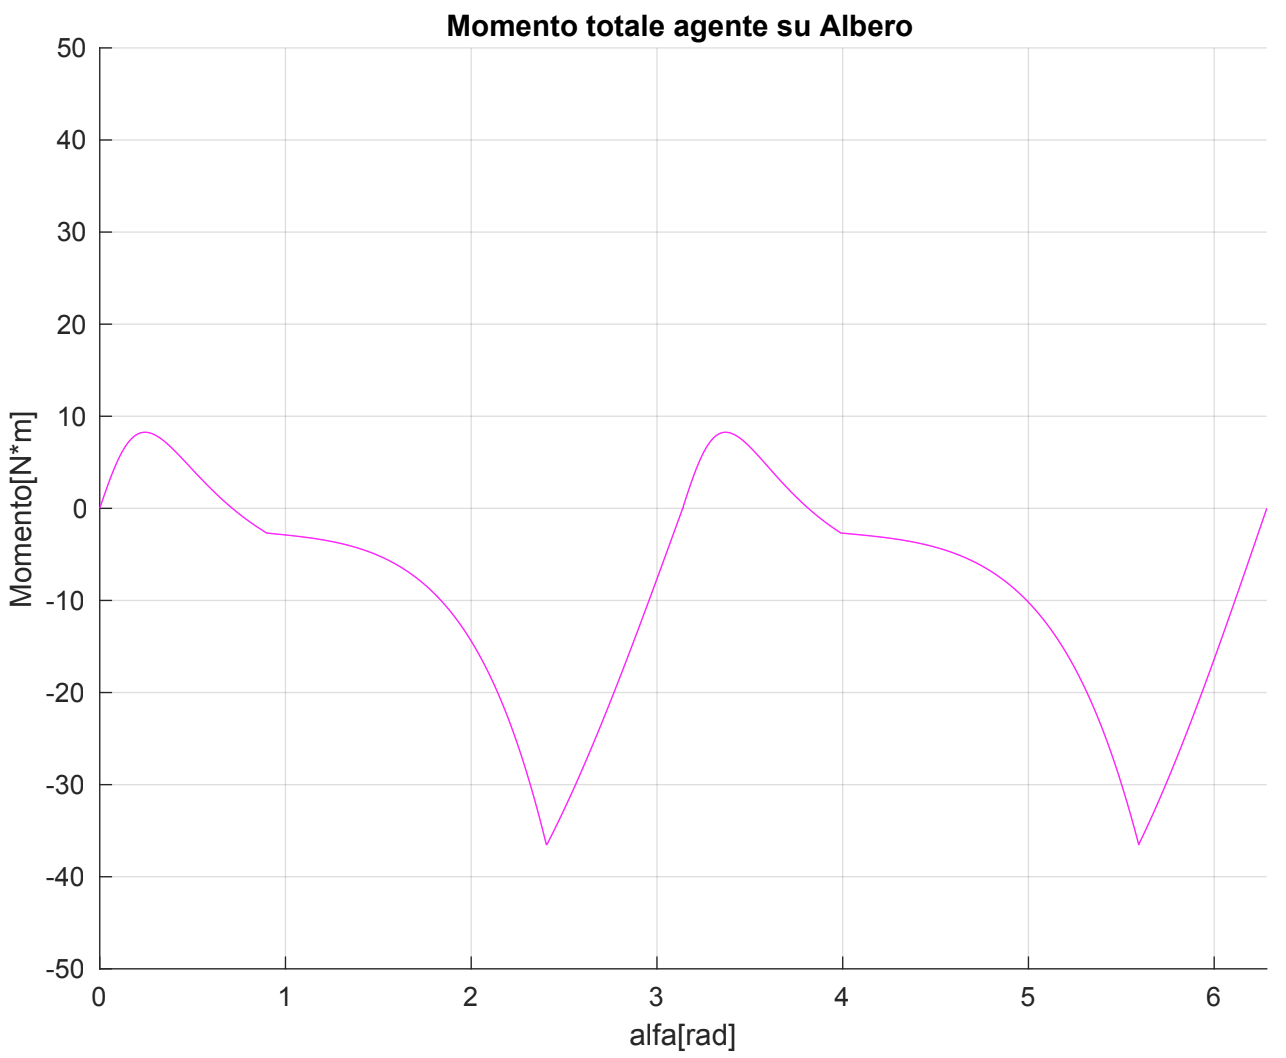
\includegraphics[scale=0.4]{Immagini/GraficoMomentoTotale.png}
    \caption{Andamento del momento torcente risultate sull'albero a gomiti}
    \label{fig:GraficoMomentoTotale}
\end{figure}
\begin{lstlisting}[frame=trBL]
%Grafico momento torcente totale

Mt2=circshift(Mt1,1000); %shifta il vettore Mt1 
                         %di meta dei valori (1000)
Mttot=Mt1+Mt2;
plot(alfatot,Mttot,'m');
xlabel('alfa[rad]'),ylabel('Momento[N*m]'),
      title('Momento totale agente su albero'),
      grid on,xlim([0 2*pi]),ylim([-50 50])
\end{lstlisting}
\subsection{Determinazione del volano che regolarizza il momento torcente}
Il volano ha il compito di assorbire l’eccesso di lavoro resistente rispetto a quello motore, sotto forma di energia cinetica, evitando che si verifichino incrementi di velocità angolare non compatibili con l’impiego a cui il sistema è destinato. \\
Come già mostrato, in Fig.\ref{fig:GraficoMomentoTotale} è riportato il momento resistente del compressore bicilindrico in esame. \\
Quando il momento resistente medio $M_{rm}$ è uguale al momento motore $M_m$, la velocità di rotazione media $\omega$ rimane costante, ma nell’intervallo in cui il momento resistente effettivo è maggiore del momento motore, la velocità istantanea di rotazione diminuisce (e quando il momento resistente è minore del momento motore, la velocità istantanea tende ad aumentare). 
\begin{figure}[h]
    \centering
    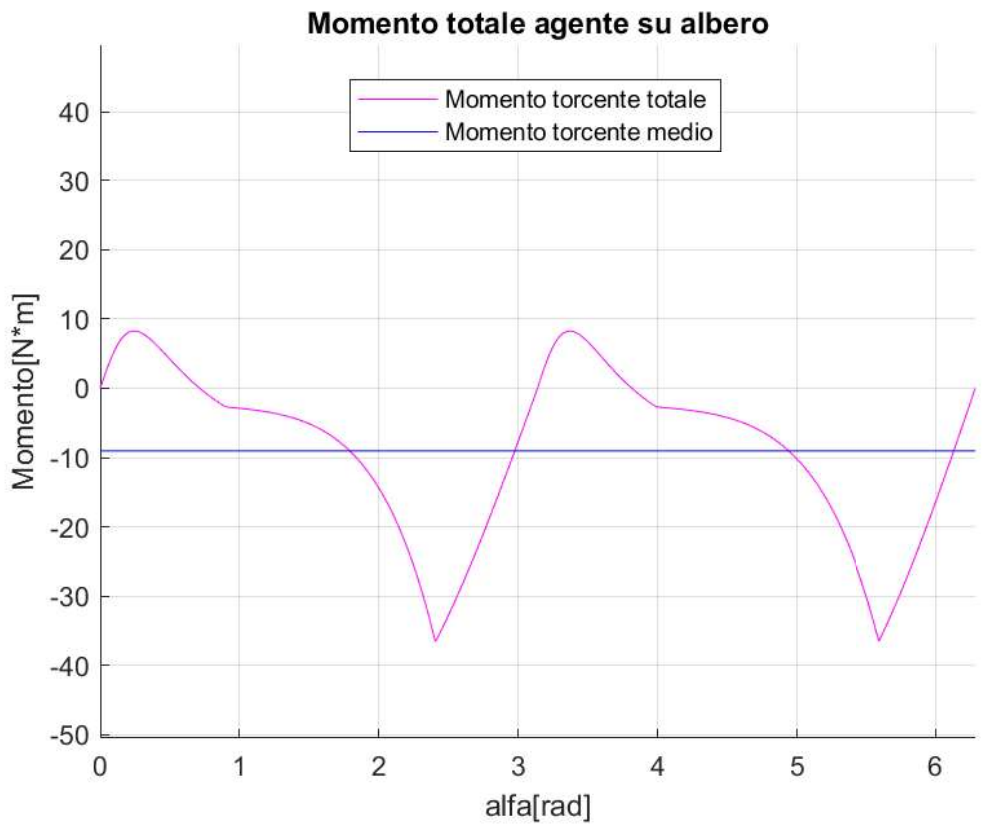
\includegraphics[scale=0.5]{Immagini/GraficoMomentoMedio.png}
    \caption{Confronto andamento momento torcente con momento torcente medio}
    \label{fig:GraficoMomentoMedio}
\end{figure}
\begin{lstlisting}[frame=trBL]
%Momento torcente medio

m=mean(Mttot); %trova la media
s=linspace(m,m,2000);
plot(alfatot,s,'b')
hold off %il vecchio grafico era stato tenuto in 
         %plot con comando hold on
\end{lstlisting}
\paragraph{Grado di irregolarità e lavoro eccedente}Indicando con $\omega_2$ la massima velocità nel periodo e con $\omega_1$ la minima, è possibile ricavare la la velocità mediante: 
\begin{equation}
    \omega=\frac{\left(\omega_1+\omega_2\right)}{2}.
\end{equation}
Si definisce grado di irregolarità nel periodo il rapporto tra la variazione di velocità e la velocità media: 
\begin{equation}
    \delta=\frac{\omega_2-\omega_1}{\omega}
\end{equation}
Da tabella I.141 del Manuale di meccanica Hoepli si stima $\delta=0.03$, relativo alle trasmissioni da officina.
\paragraph{Calcolo del momento di inerzia del volano}
Indicando con N [W] la potenza e con n [giri/min] i giri al minuto dell’albero motore, si ha:
\begin{equation}
    N=M_{rm}\omega=M_{rm}\frac{2\pi n}{60}
\end{equation}
da cui si può ricavare il lavoro medio in un giro: 
\begin{equation}
    M_{rm}2\pi=60\frac{N}{n}.
    \label{LavoroMedioGiro}
\end{equation}
Il lavoro massimo di fluttuazione risulta essere pari a: 
\begin{equation}
    L_F=\int_{\alpha_A}^{\alpha_B}{(M_r-}M_{rm})d\alpha\ =\frac{1}{2}I\left(\omega_2^2-\omega_1^2\right)
    \label{LavoroFluttuazione}
\end{equation}
dove I rappresenta il momento di inerzia di tutte le masse rotanti rispetto all’asse di rotazione.\\
\begin{figure}[h]
    \centering
    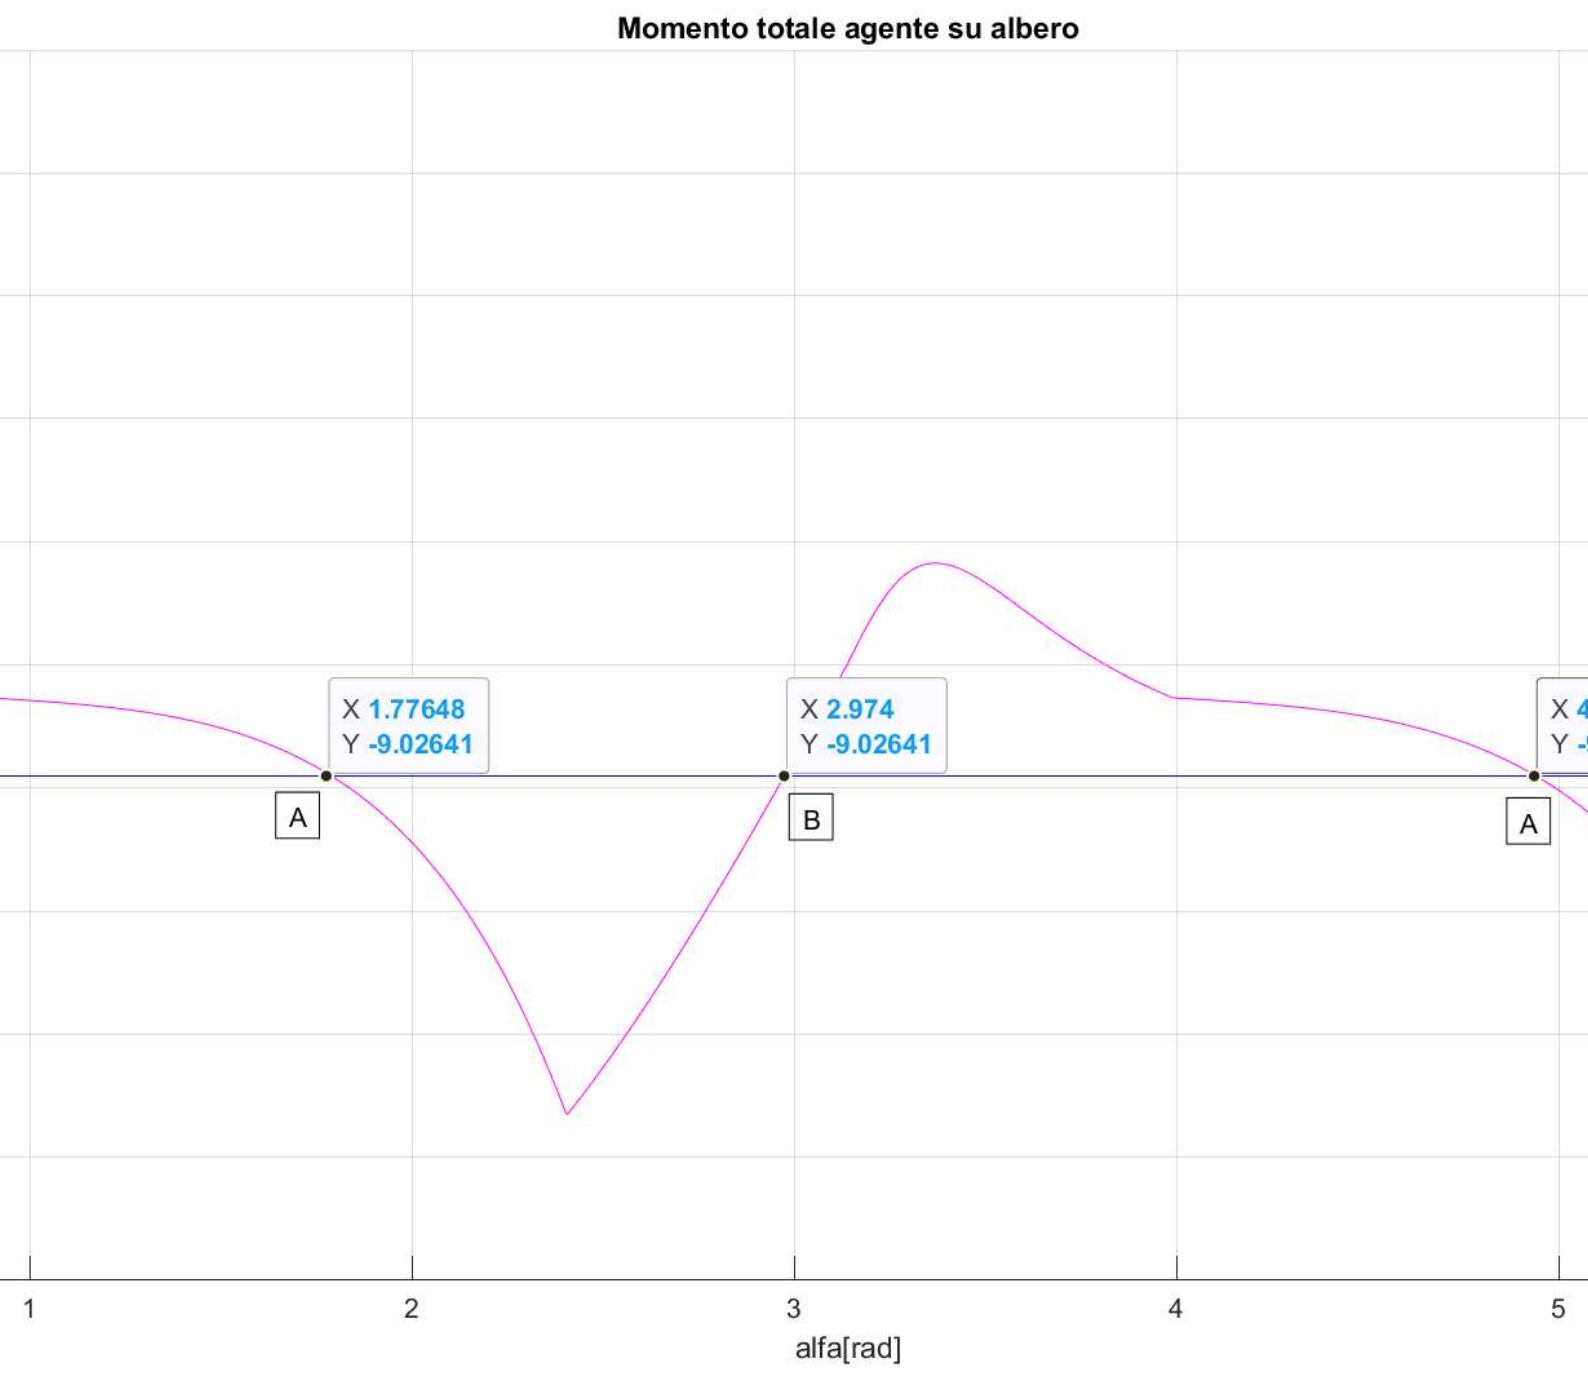
\includegraphics[scale=0.3]{Immagini/GraficoPuntiMomento.png}
    \caption{Punti A e B indicati in formula \ref{LavoroFluttuazione}}
    \label{fig:GraficoPuntiMomento}
\end{figure}
\\
In prima approssimazione si ritiene preponderante il momento di inerzia del volano rispetto alle altre masse e, quindi, nella trattazione I sarà il momento di inerzia del volano.\\
\\
Concretamente il lavoro massimo di fluttuazione corrisponde alla massima area sottesa tra la curva del momento resistente $M_r$ e il suo valore medio $M_{rm}$.\\
Esso può essere anche espresso come frazione del lavoro medio in un giro: 
\begin{equation}
    L_F=\varphi M_r2\pi=\varphi\ 60\frac{N}{n}
    \label{FrazioneLavoroMedio}
\end{equation}
in cui $\varphi$ è il coefficiente di fluttuazione, dipendente dal tipo di applicazione e ricavabile tramite tabelle. \\
Per i successivi calcoli considereremo un $\varphi$ pari a 0,15. 
\paragraph{Calcolo momento di inerzia del volano}Tenendo conto delle eq.(\ref{FrazioneLavoroMedio}), (\ref{LavoroFluttuazione}) e (\ref{LavoroMedioGiro}), può essere scritta:
\begin{equation}
    \varphi\ 60\frac{N}{n}=I\omega^2
\end{equation}
da cui si può ricavare il momento di inerzia del volano in funzione della potenza, del coefficiente di fluttuazione e del grado di irregolarità:
\begin{equation}
    I=\frac{2\pi\varphi N}{\delta \omega^3}.
\end{equation}
Facendo i calcoli si ottiene che $I=\left|10,9\cdot10^{-3}\right|\ kgm^2$. 
Noto il raggio del volano pari a $r=150\ mm$, è possibile determinare la massa del volano come: 
\begin{equation}
    m=\frac{I}{r^2}=0,5\ kg.
\end{equation}
I risultati ottenuti sono compatibili con quelli ricavati mediante SOLIDWORKS.
\begin{figure}[h]
    \centering
    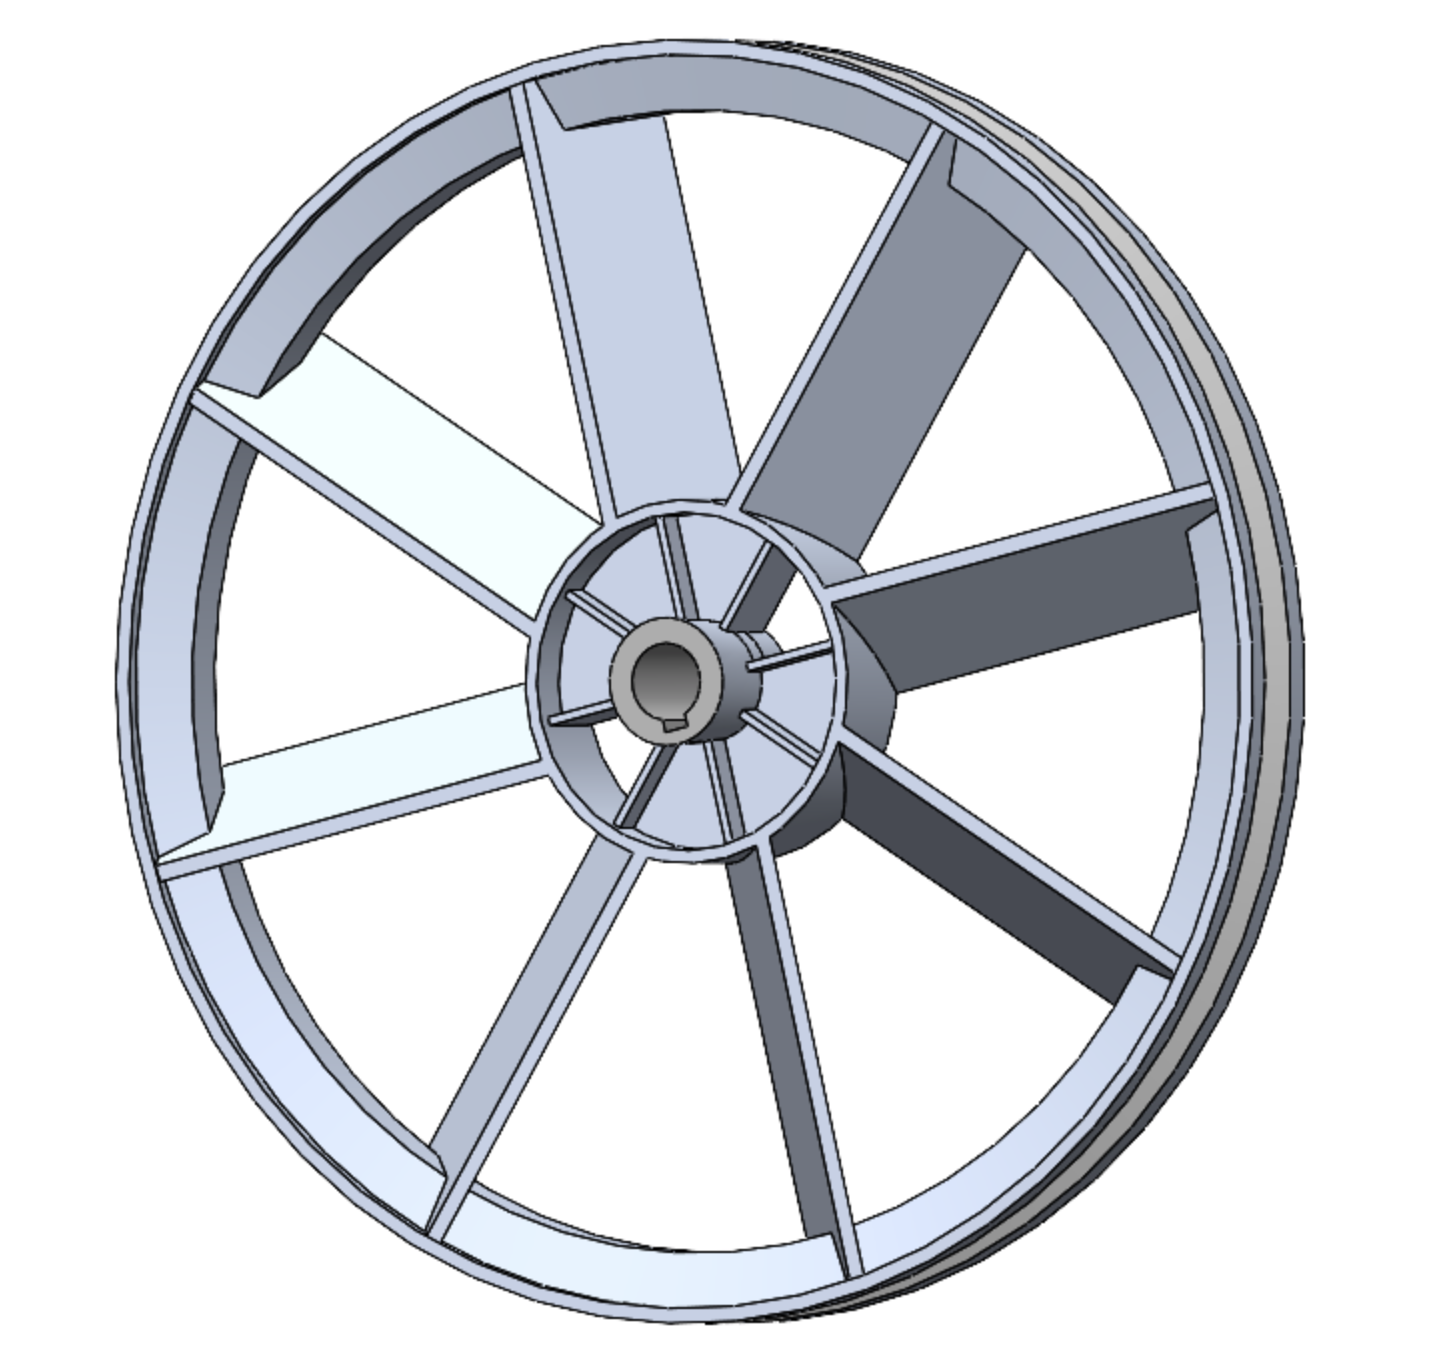
\includegraphics[scale=0.2]{Immagini/Volano.png}
    \caption{Modello CAD SOLIDWORKS del volano}
    \label{fig:Volano}
\end{figure}
\begin{figure}[h]
    \centering
    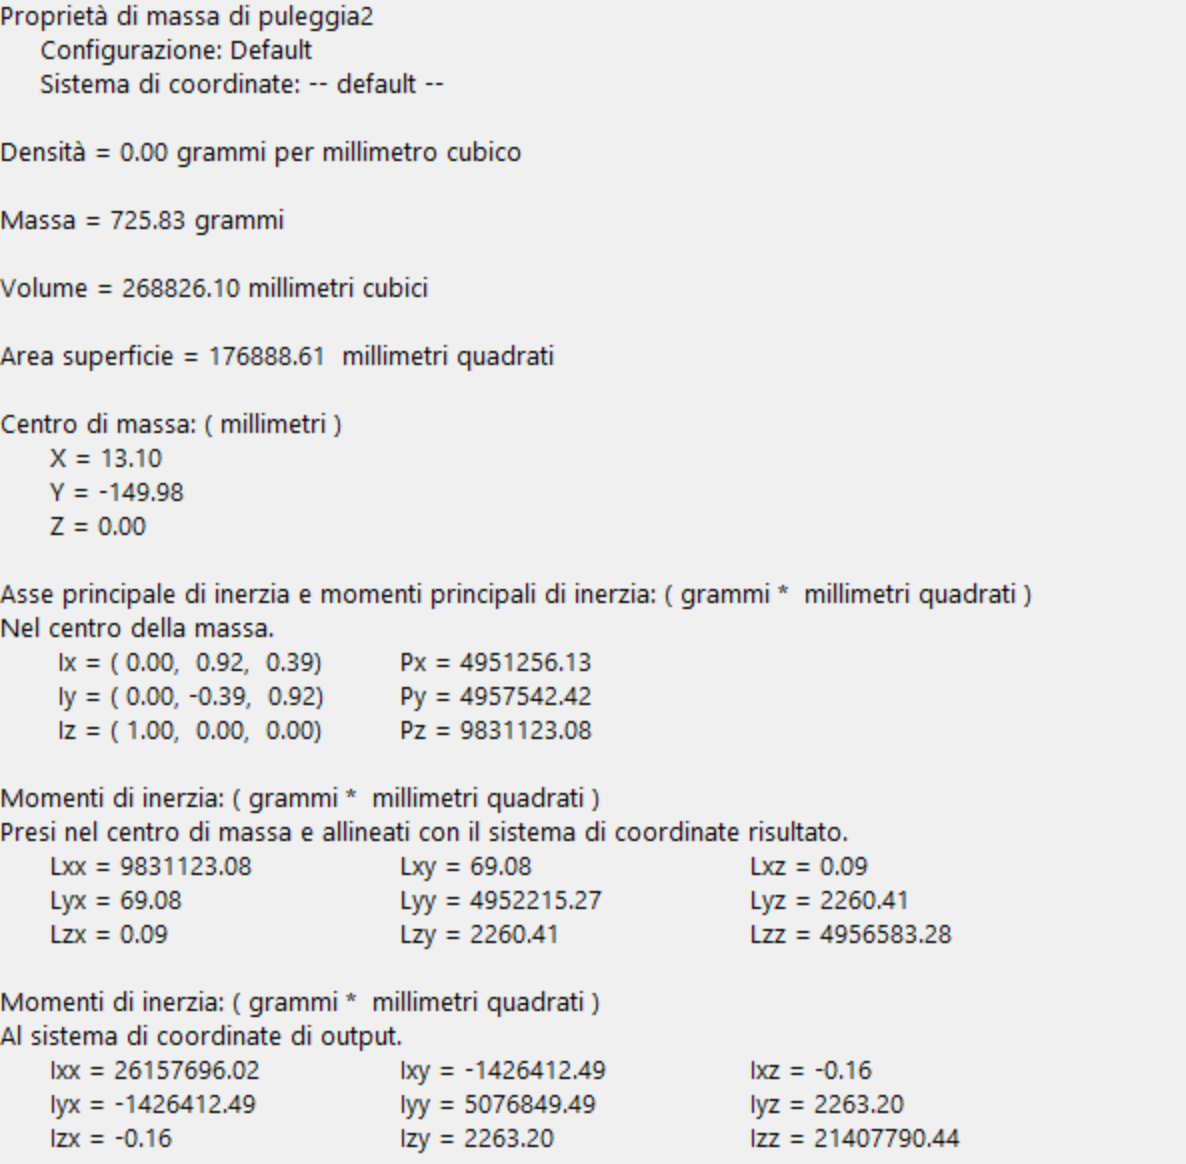
\includegraphics[scale=0.5]{Immagini/CaratteristicheVolano.png}
    \caption{Caratteristiche del volano ricavate mediante software SOLIDWORKS}
    \label{fig:CaratteristicheVolano}
\end{figure}
\newpage
È possibile, inoltre, determinare la velocità periferica dei punti più esterni della corona che non può superare limiti ben precisi, per non creare eccessive sollecitazioni nel materiale.\\
Nella maggior parte dei casi si tende a mantenere tale velocità intorno ai 30 - 35 m/s. Nel caso specifico in esame si ottiene una velocità periferica pari a:
\begin{equation}
    v=\omega r=24,25\ m/s
\end{equation}
rientrante nel range di sicurezza. 
\subsection{Determinazione del motore elettrico}
Noto il valore medio del momento resistente, sarà possibile determinare la potenza motrice richiesta per il funzionamento del compressore alla macchina elettrica: 
\begin{equation}
    N=M_{rm}\omega=1454,64\ W=1,45\ kW.
\end{equation}
Considerando un rendimento complessivo della trasmissione a cinghia pari a $\eta=0,96$ si ottiene che la potenza che il motore deve complessivamente fornire corrisponde a: 
\begin{equation}
    N_{eff}=\frac{N}{\eta}=1,5\ kW.
\end{equation}
Da catalogo Nuova Omas è stato scelto un motore con caratteristiche idonee. 
\begin{figure}[h]
    \centering
    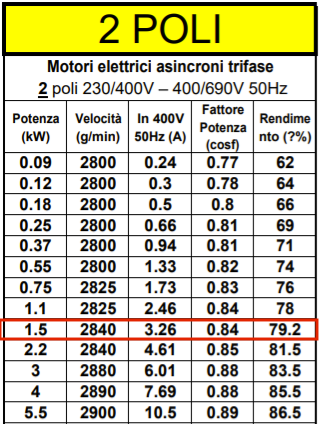
\includegraphics[scale=0.6]{Immagini/CatalogoMotoreElettrico.png}
    \caption{Catalogo Nuova Omas per la scelta del motore elettrico}
    \label{fig:CatalogoMotoreElettrico}
\end{figure}
\subsection{Calcolo della trasmissione con cinghia trapezoidale}
Le cinghie trapezoidali sono così chiamate per la forma della loro sezione, che si presenta come nella figura sottostante (Fig.\ref{fig:CinghiaTrapezoidale}).
\newpage
\begin{figure}[h]
    \centering
    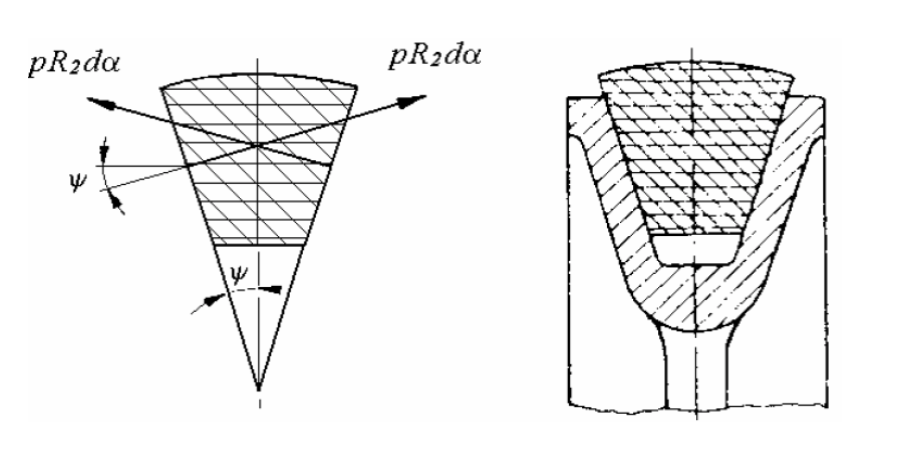
\includegraphics[scale=0.4]{Immagini/CinghiaTrapezoidale.png}
    \caption{Vista di una cinghia trapezoidale in sezione}
    \label{fig:CinghiaTrapezoidale}
\end{figure}
La cinghia è costruita in elastomero, con uno o più strati di trefoli in poliestere ed un rivestimento esterno protettivo di tela impregnata con elastomero. Il materiale con cui la cinghia è realizzata permette di raggiungere elevati coefficienti di attrito, ma è soprattutto il modo con  cui essa esercita la sua azione sulla puleggia, che contribuisce ad accrescere l’attrito con quest’ultima (contatto con le superfici laterali di una gola a V).\\
Le cinghie di trasmissione trapezoidali sono le più utilizzate per la trasmissione di potenza, perché risolvono allo stesso tempo il problema dell’allineamento e parzialmente dello slittamento. \\
Se le potenze in gioco sono elevate, è possibile utilizzare sulla stessa puleggia (con scanalature multiple) più cinghie trapezoidali.\\
\\
I dati fino ad ora noti ed indispensabili per la progettazione del sistema di trasmissione sono: 
\begin{itemize}
    \item Velocità di rotazione albero a gomiti: $n = n_2 = 1540\ rpm$ 
    \item Velocità di rotazione albero motore elettrico: $n_1 = 2840\ rpm$
    \item Diametro esterno puleggia compressore: $d_{2e} = 300\ mm$
    \item Diametro interno puleggia compressore: $d_{2i} = 274\ mm$
    \item Diametro medio puleggia compressore: $d_{2m}=\frac{d_{2e}+d_{2i}}{2}=287\ mm$
    \item Potenza trasmessa: $P = 1,5\ kW$
    \item Velocità periferica media puleggia compressore: $v_{2m}=\frac{2\pi n_2}{60}\ \frac{d_{2m}}{2}=23,14\ m/s$ (gamma di velocità ottimale varia fra i 5 e i 50 m/s).
\end{itemize}
\begin{figure}[h]
    \centering
    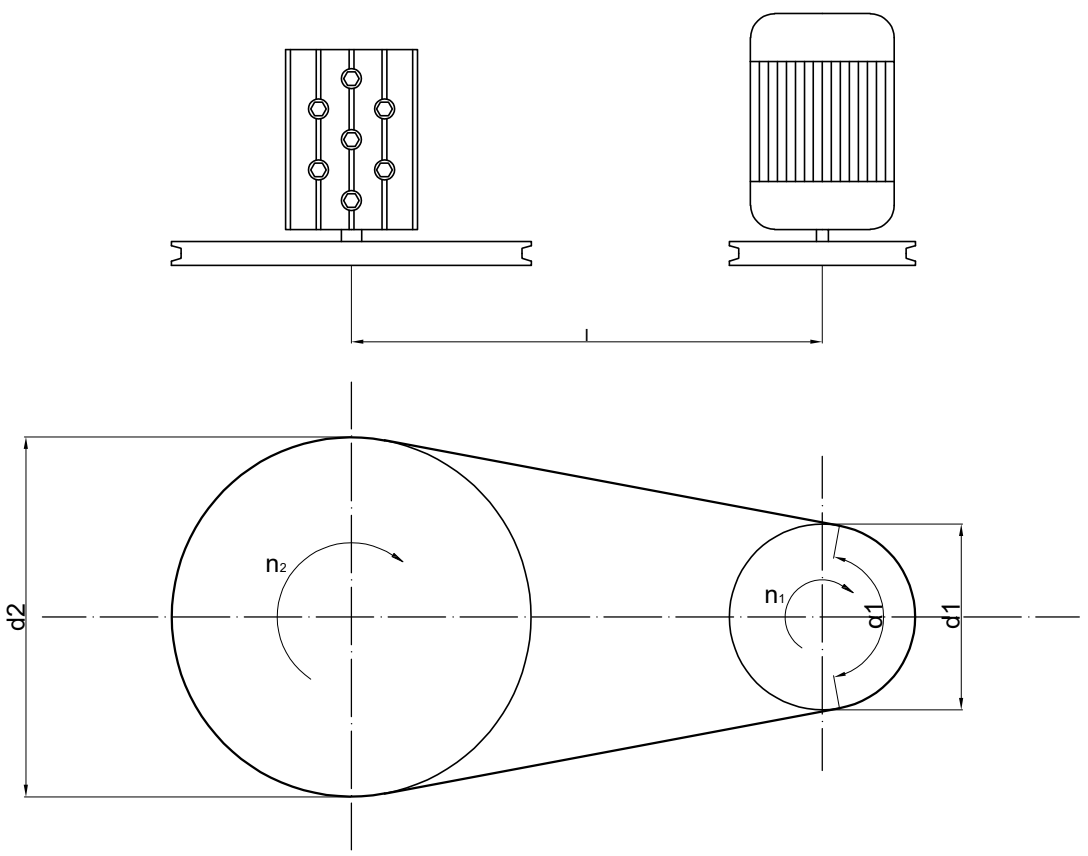
\includegraphics[scale=0.55]{Immagini/SchemaMontaggio.png}
    \caption{Schema di montaggio delle pulegge}
    \label{fig:SchemaMontaggio}
\end{figure}
Note le velocità di rotazione del motore elettrico e dell’albero motore del compressore, è possibile stimare il rapporto di trasmissione del sistema meccanico come:
\begin{equation}
    \tau=\frac{n_2}{n_1}=1,844
\end{equation}
da cui è possibile ricavare il diametro medio della puleggia associata alla macchina elettrica, ovvero quella più piccola:
\begin{equation}
    d_{1m}=\frac{d_{2m}}{\tau}=155,6\ mm.
\end{equation}
Ottenuti questi parametri si può quindi procedere nella progettazione della trasmissione a cinghia trapezoidale, riferendosi alle procedure indicate sul catalogo Pi Belt Pizzirani. \\
Si inizia supponendo un opportuno interasse tra le due pulegge scelto fra un range di valori raccomandati, in funzione dei diametri medi delle due pulegge. 
\begin{equation}
    0,7(d_{1m}+d_{2m})<I<2(d_{1m}+d_{2m})=309,83\ mm<I<885,24\ mm\ 
\end{equation}
Si sceglie un interasse teorico pari a $I_{th}=450\ mm$.
Da questo sarà quindi poi possibile determinare la lunghezza complessiva dell’organo flessibile mediante la seguente relazione: 
\begin{equation}
    L_{th}=2I_{th}+1,57\left(d_{1m}+d_{2m}\right)+\frac{\left(d_{2m}-d_{1m}\right)^2}{4 I_{th}}=1604,5\ mm
\end{equation}
Prima di determinare la lunghezza reale della cinghia sarà però necessario determinarne la tipologia costruttiva, in base alle dimensioni note della puleggia reperibili mediante valutazione del disegno su SOLIDWORKS.\\
\begin{figure}[h!]
    \centering
    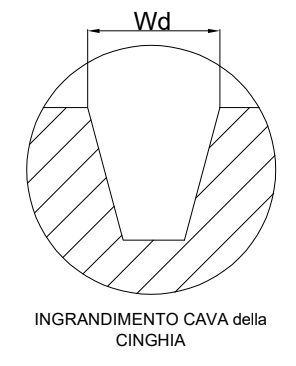
\includegraphics[scale=0.6]{Immagini/IngrandimentoCinghia.png}
    \caption{Ingrandimento della cava della cinghia}
    \label{fig:IngrandimentoCinghia}
\end{figure}

Poiché risulta $W_d=13\ mm$ è stata scelta una cinghia di tipologia B con le caratteristiche dimensionali rappresentate sotto in tabella.\\
\begin{figure}[h]
    \centering
    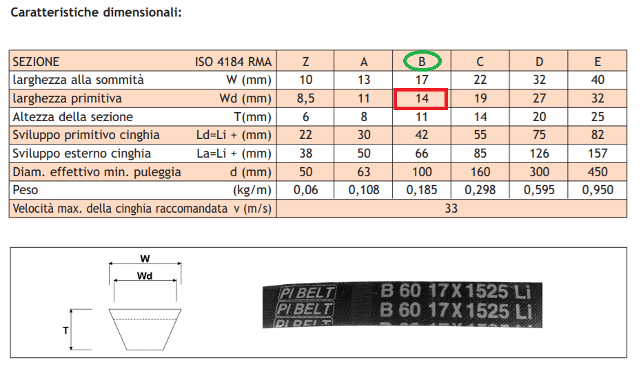
\includegraphics[scale=0.7]{Immagini/CaratteristicheDimensionaliCinghia.png}
    \caption{Dimensionamento cinghia da catalogo}
    \label{fig:CaratteristicheDimensionaliCinghia}
\end{figure}

A questo punto è possibile individuare la lunghezza reale della cinghia, scegliendola sempre dal medesimo catalogo.\\
\newpage
\begin{figure}[h]
    \centering
    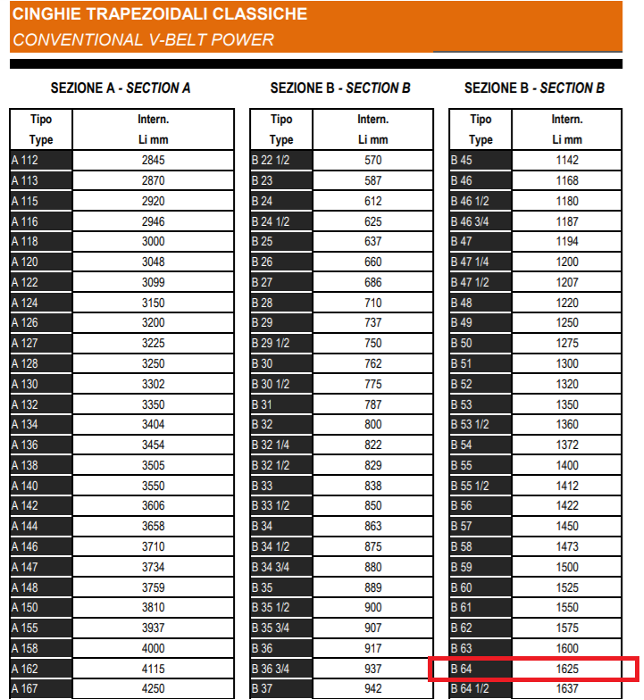
\includegraphics[scale=0.65]{Immagini/SceltaCinghia.png}
    \caption{Selta della cinghia da catalogo}
    \label{fig:SceltaCinghia}
\end{figure}

La cinghia scelta è la B64, con una lunghezza pari a: 
\begin{equation}
    L=1625\ mm.
\end{equation}
Da questa si ricava il valore reale dell’interasse, che inizialmente era solo stato ipotizzato, come: 
\begin{equation}
    I=\frac{L-1,57\left(d_{1m}+d_{2m}\right)}{2}-\frac{\left(d_{2m}-d_{1m}\right)^2}{4\left[L-1,57\left(d_{1m}+d_{2m}\right)\right]}=462\ mm
\end{equation}
Si è quindi caratterizzato dimensionalmente il sistema di trasmissione meccanica a cinghia.\\
\\
Si può poi proseguire con la valutazione del pretensionamento da conferire alla cinghia, per garantire la trasmissione del moto fra le due pulegge evitando slittamenti. 
\paragraph{Calcolo del pretensionamento}Nuovamente dal catalogo è possibile quantificare il valore della forza di pretensionamento da fornire al sistema di trasmissione, come esplicitato dalla seguente relazione: 
\begin{equation}
    T=\frac{50\left(2,5-a\right) P}{a N v_{2m}}+Kv_{2m}^2
\end{equation}
dove: 
\begin{itemize}
    \item a: fattore di correzione dell’arco di contatto (ricavabile dalla Fig.\ref{fig:ArcoDiContatto}) 
    \item K: coefficiente relativo alla massa lineare delle cinghie (ricavabile dalla Fig.\ref{fig:CoefficienteK})
    \item N = numero di pulegge (supposto inizialmente N = 1).
\end{itemize}
Quindi con $a=0.96$, $K=0,019$ e $N=1$ si ottiene una forza di pretensionamento pari a: 
\begin{equation}
    T=52,1\ N.
\end{equation}
Questo pretensionamento T genera sull’albero una forza statica di modulo: 
\begin{equation}
    R_s=2NT\cos\left(90^\circ-\frac{\alpha_1}{2}\right)=103,05\ N
\end{equation}
con $\alpha_1=163^\circ$, arco di contatto della cinghia sulla puleggia minore, ricavato dalla Fig.\ref{fig:ArcoDiContatto}.
\begin{figure}[h]
    \centering
    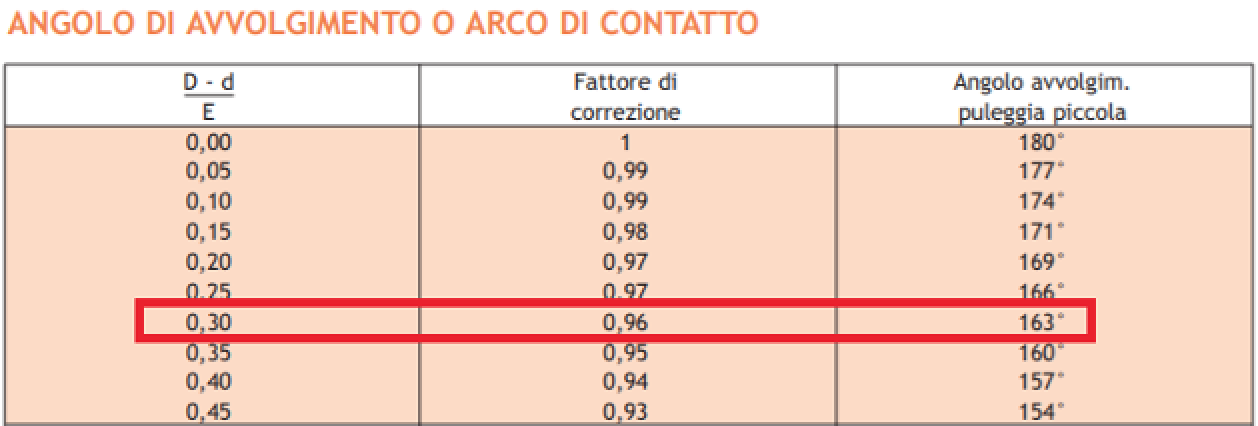
\includegraphics[scale=0.54]{Immagini/ArcoDiContatto.png}
    \caption{Tabella per la scelta del fattore di correzione dell'arco di contatto}
    \label{fig:ArcoDiContatto}
\end{figure}
\newpage
\begin{figure}[h]
    \centering
    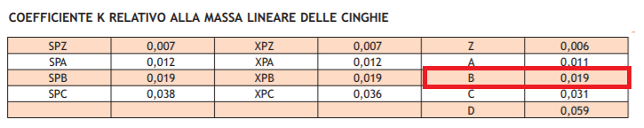
\includegraphics[scale=0.8]{Immagini/CoefficienteK.png}
    \caption{Tabella per la scelta del coefficiente K relativo alla massa lineare delle cinghie}
    \label{fig:CoefficienteK}
\end{figure}
\paragraph{Verifica della potenza trasmissibile dalla cinghia} Al termine della progettazione si verifica che il sistema flessibile scelto riesca a trasmettere la potenza necessaria al compressore per il suo funzionamento. \\
Si può stimare la potenza massima trasmissibile dalla cinghia con la seguente formulazione, estraibile dal catalogo: 
\begin{equation}
    P_{amm}=a{C}_{l}\left(P_{nom}+P_{aggiuntiva}\right)
\end{equation}
con
\begin{itemize}
    \item a = 0,96 (già ottenuto in precedenza) 
    \item $C_l$: fattore correttivo della lunghezza (ricavabile dalla Fig.\ref{fig:FattoreDiCorrezioneDellaLunghezza}) 
    \item $P_{nom}$: potenza massima complessiva che può essere trasmessa alla cinghia (ricavabile da Fig.\ref{fig:PotenzaTrasmissibile})
    \item $P_{aggiuntiva}$: potenza aggiuntiva alla $P_{nom}$ (ricavabile anch’essa da Fig.\ref{fig:PotenzaTrasmissibile}).
\end{itemize}
\begin{figure}[h]
    \centering
    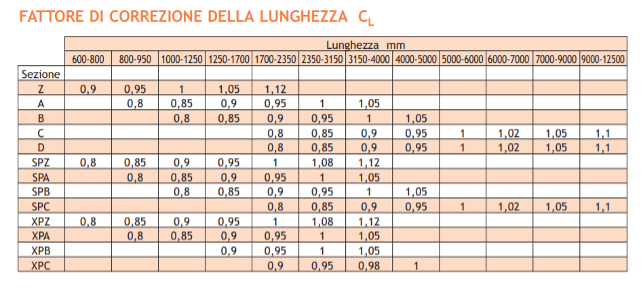
\includegraphics[scale=0.7]{Immagini/FattoreDiCorrezioneDellaLunghezza.png}
    \caption{Tabella del fattore di correzione della lunghezza $C_l$}
    \label{fig:FattoreDiCorrezioneDellaLunghezza}
\end{figure}
\begin{figure}[h]
    \centering
    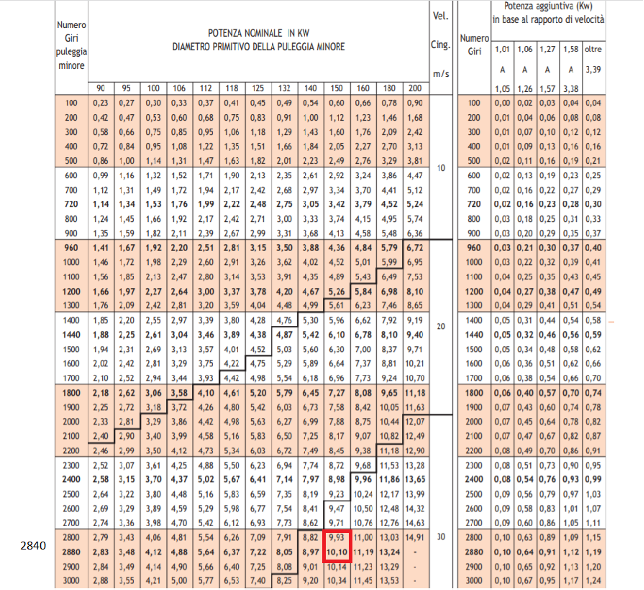
\includegraphics[scale=0.9]{Immagini/PotenzaTrasmissibile.png}
    \caption{Potenza nominale trasmissibile dalla cinghia}
    \label{fig:PotenzaTrasmissibile}
\end{figure}

Con $a=0.96$, $C_l=0,85$, $P_{nom}\cong10\ kW$ e $P_{aggiuntiva}\cong 1,10\ kW$, si ottiene:
\begin{equation}
    P_{amm}=9,06\ kW.
\end{equation}
Risulta quindi verificato che: 
\begin{equation}
    P_{amm}=9.05\ kW>P=1,5\ kW
\end{equation}
Il sistema adottato è quindi idoneo a questa applicazione, ed è verificata l’ipotesi iniziale di un’unica cinghia, quindi N =1. 


